% arara: lualatex
% LTeX: enabled=false

\documentclass[12pt]{memoir}

\usepackage{construcao-pintura-cinema-preamble}
\usepackage{blucher-arroz-post-production}

\title{A Construção da Imagem na Pintura pelo Olhar do Cinema}
\author{Odette de Queiroz Boudet Fernandes}
\local{Porto}
\curso{Faculdade de Belas Artes da Universidade do Porto}
\descricaodotrabalho{Dissertação para obtenção de grau de Mestre em Artes Plásticas \\ Especialização em Pintura}
\orientador{Professora Doutora Joana Rêgo}
\coorientador{Professora Doutora India Mara Martins}


\begin{document}

\selectlanguage{brazilian}

\frontmatter

\cover

\titlepage

\thispagestyle{empty}


\chapter*{Agradecimentos}

\thispagestyle{empty}

Ao Carlos Caldas, o Charlie, meu companheiro e amor desta vida, pelo
incentivo e apoio incondicional a este e a todos os projetos artísticos
que tenho realizado.

Aos meus filhos queridos, Julia e Tarso, que me ajudam a atualizar o
olhar e ter esperança em um mundo melhor.

À minha orientadora Joana Rego, que acompanhou esta pesquisa desde seu
processo embrionário,~com as primeiras pinturas em Portugal, me
apresentando e inspirando com referências importantes, como~a dos
escritos inacabados de Walter Benjamin, deixados em uma mala.

À minha coorientadora India Mara Martins, especialmente pelo acolhimento
na disciplina Teorias da imagem e a construção do olhar, no PPGCine-Uff,
um momento importante para a retomada dos estudos e da escrita
vinculados ao cinema e audiovisual.

À Rosa e Ana Maria que além de cuidar das condições físicas do Ateliê de
Pintura da Boa Hora, nos apoiavam afetivamente garantindo a paz
necessária a este espaço compartilhado de criação.

À Isabel Barroso, pela sua disponibilidade em orientar sobre as
ferramentas disponíveis para a formatação deste trabalho, junto ao SDI
da Biblioteca da \ac{fbaup}.

Aos professores e orientadores das instituições, cursos e consultorias,
que iluminaram este percurso, representados aqui por Alberto Fernandes, Ana Kothe, Caio
Pacela, João Magalhães, Jozias Benedito, Luiz Ernesto, Luana Manhães,
Monique Queiroz, Shannon Botelho e Rafael Bteshe.

Aos amigos do cinema e da pintura, do Brasil e de Portugal, e não
somente estes, que se fazem representar aqui pelos que me apoiaram de
perto neste percurso, como Damian Ross, Lena Mendes, Marcela Pedersen, Marcia
Campbell, Maria de Fátima Ginicolo, Stella Margarita, Maia Bueloni,
Raquel Dora Pinho, Ricardo Larangeira e Taty Arruda.

\clearpage

\thispagestyle{abstract}

\begin{abstract}
	O debate sobre como a imagem é construída e se apresenta no mundo
	atual, está cada vez mais presente em muitos campos de investigação. O
	crescente interesse de pessoas em se iniciar nas artes visuais, cuja
	cultura visual não se relaciona diretamente ao mundo da pintura,
	justifica a escolha deste tema. Com a pergunta inicial sobre como a
	tela branca será abordada para expressar nossas próprias ideias,
	objetivamos investigar como utilizar~o olhar característico do cinema,
	no método processual da construção de uma pintura, ou de outra forma,
	no exercício da atividade do pintor. Partindo do contexto histórico do
	nascimento do cinema, foi realizada uma pesquisa bibliográfica
	envolvendo os autores Jacques Aumont, André Gardies, Delfim Sardo, e
	outros que, em suas abordagens, vinculam o olhar característico do
	cinema e da pintura a conceitos de movimento, espaço e \emph{óptica}.
	Investigamos o~uso~de referências para projetos artísticos pessoais,
	com origem em outros campos, por meio da trajetória de duas pintoras
	brasileiras: Lucia Laguna e Cristina Canale. A metodologia de nossa
	pesquisa foi a conjugação de uma revisão bibliográfica com a
	experimentação, de ordem processual e prática, realizada no ateliê do
	Mestrado em Artes Plásticas da Faculdade de Belas Artes da \ac{uporto}. A
	partir do estudo realizado neste trabalho e, nas reflexões sobre o uso
	de projeção de imagens na realização de esboços, concluímos ser
	relevante propor e disseminar métodos alternativos ao ensino acadêmico
	de pintura, alinhados à poética de artistas que trabalham no âmbito da
	arte contemporânea.

  \medskip
	\noindent\emph{\bfseries Palavras-chave:} Construção da imagem; olhar; cinema; pintura; movimento; espaço.
\end{abstract}

\clearpage

\thispagestyle{abstract}

\renewcommand{\absnamepos}{flushright}
\begin{otherlanguage}{english}
	\begin{abstract}

		The debate on how the image is constructed and presented in today's
		world is increasingly present in many fields of investigation. The
		growing interest in embarking on
		visual arts, whose visual culture is not directly related to the world
		of painting, justifies the choice of this theme. Starting with the question 
    of how the white canvas will
		be approached to express our own ideas, we  investigate how to
		use the characteristic visual style of cinema, whether, in the
		procedural method of the construction~of a painting or, 
    in the exercise of the painter's activity. We provide
		historical context from the
		birth of~cinema, through authors such as Jacques Aumont, André Gardies,
		Delfim Sardo, and others who, in their approaches, link the
		characteristic looks of cinema and painting to concepts of movement,
		space and optics. We then investigate the use of references for
		personal artistic projects, originating in other fields, through the
		trajectory of two Brazilian painters: Lucia Laguna and Cristina Canale.
		Our research methodology 
		combined this bibliographic review with experimentation, of a
		procedural and practical nature, carried out in the studio of the
		Master's in Plastic Arts at the Faculty~of Fine Arts
    in \ac{uporto}. From the study carried out in this work and in our
		reflections on the use of~image projection in the creation of sketches,
		we conclude that it is relevant to propose and disseminate alternative
		methods to the academic teaching of painting, in line with the poetics
		of artists who work in the field of contemporary art.

    \medskip
		\noindent\emph{\bfseries Keywords:} Image construction; view; cinema; painting; movement; space.
	\end{abstract}
\end{otherlanguage}

\clearpage

\tableofcontents*

\clearpage

\listoffigures*

\clearpage


\listofquadros*


\chapter*{Lista de Abreaviatura}

\begin{acronym}
	\acro{apa}[APA]{Associação Americana de Psicologia}

  \acro{app}[App]{Aplicativo}

	\acro{eav}[EAV]{Escola de Artes Visuais do Parque Lage}

	\acro{fbaup}[FBAUP]{Faculdade de Belas Artes da Universidade do Porto}

	\acro{ppgcine-uff}[PPGCine-UFF]{Programa de pós-graduação em cinema e
		audiovisual da Universidade Federal Fluminense}

	\acro{sdi}[SDI]{Sistema de Documentação e Informação}

	\acro{ufrj}[UFRJ]{Universidade Federal do Rio de Janeiro}

	\acro{uporto}[UPORTO]{Universidade do Porto}
\end{acronym}

\clearpage

\begin{authornote}
	Esta dissertação foi escrita em conformidade com a norma técnica da
	APA, 7\textordfeminine~edição. Diagramação foi feita em \LaTeX\ por Tarso Boudet Caldas.

	Ao buscar um consenso entre acordos ortográficos sobre a palavra
	óptico/ótico, relativo ao olho, encontrei informações sobre a grafia da
	palavra óptica \emph{s.f.}~ciência da visão e ótica \emph{s.f.}~ciência
	da audição. Dicionários reconhecidos, inseridos no contexto do Acordo
	Ortográfico, divergem quanto à grafia da consoante p, por ser muda na
	pronúncia individual dos vários falantes de língua portuguesa. Em
	Portugal não se usa óptica, enquanto no Brasil são aceitas as duas
	grafias, embora mantenha-se a distinção entre os significados
	referentes a visão e audição \parencite{ILLLP2015optico}.

	Diante das várias possibilidades de escrita para uma única palavra,
	deixo de lado as discussões que insistem em permanecer, referentes à
	língua que compartilhamos neste espaço de escrita e opto por adotar o
	português materno, do Brasil, com o qual me expresso desde que nasci.
	Assim espero comunicar melhor as imagens, que tanto importam nesta
	pesquisa.
\end{authornote}


\mainmatter

\counterwithout{figure}{chapter}
\counterwithout{figure}{chapter}
\counterwithout{footnote}{chapter}

\chapter*{Introdução}\label{introducao}
\pagestyle{introducao}

O debate e as reflexões sobre a imagem, como ela é construída e se
apresenta no mundo atual, estão cada vez mais presentes em muitos
campos de investigação. A escolha de um ponto de vista para se falar
sobre um assunto tão amplamente discutido, não é uma tarefa fácil. Um
dos problemas mais comuns, para aqueles que decidem mergulhar no
complexo mundo da pintura, é decidir de que forma a tela branca será
abordada para expressar aquilo que, por hipótese, seria uma
representação de suas ideias. A distância entre o suporte e a mão do
artista é aparentemente curta, mas existe um longo percurso, que tem
sido descrito pela história da pintura ocidental, até que a obra seja
considerada acabada e apta a enfrentar o olhar do outro. Além disto,
cada vez mais pessoas, cujo repertório visual não necessariamente se
relaciona ao mundo da pintura, demonstram interesse em se iniciar no
mundo das artes visuais. No sentido inverso,
\textcquote[131]{sabino2000pintura}{muitos artistas possuem uma vontade
	criativa, em determinado momento de seu percurso, de usar suportes e
	meios de expressão exteriores ao da própria pintura}

O caminho para a busca do autoconhecimento e a consequente seleção de
meus principais interesses de investigação foram estratégias decisivas
para dar clareza a questionamentos para os quais não tinha respostas. A
lembrança do fazer experimental, por meio de uma câmera de filme Super
8, durante a graduação em cinema nos anos 1980 abriu espaço para as
questões que permanecem até hoje, que se resumem ao problema do olhar
mediado ou não por um dispositivo.

A presente dissertação é o resultado de uma investigação durante o
curso de mestrado em artes plásticas da Faculdade de Belas Artes da
Universidade do Porto e, principalmente, da minha busca pessoal,
enquanto artista/investigadora, por delimitar um dos campos de pesquisa
que considero mais importantes no exercício da atividade do pintor, que
é a construção de uma imagem. As reflexões sobre a prática em ateliê,
aprofundadas ao longo do período de estudos deste mestrado, trouxeram à
tona as seguintes indagações teórico-práticas recorrentes, que já se
apresentavam muitos anos antes do início do curso:

\begin{itemize}
	\item Qual a possibilidade de se utilizar o olhar característico do cinema,
	      no método processual da construção de uma pintura?

	\item Como se movimentam os olhos dos espectadores diante de uma pintura?

	\item Como é feita a seleção, pelos pintores, das referências que apoiarão
	      seus projetos?
\end{itemize}
\noindent E, na busca de compreender e lidar com estes dois universos do meu
percurso pessoal, passei a investigar as possíveis relações da pintura
com o cinema e do cinema com a pintura.

\begin{figure}[t]
  \caption{\artname{\odette}{Ando}{2012}}

	\includegraphics[width=2.8in]{odette-ando-2012.pdf.compressed.pdf}
  \figurenote{\series{Construir}. \oleo. \artsize{104 x 97}.}
\end{figure}

Meu interesse pela construção da imagem na pintura surge na Escola de
Artes Visuais do Parque Lage, no Rio de Janeiro, a partir de 2011,
quando tive o primeiro contato com o estudo prático de pintura, onde o
foco principal era a pintura contemporânea. Participei de vários cursos
livres, marcados pela didática de professores pintores que integraram o
grupo \emph{Como vai você Geraçāo 80.} Conforme aponta
\textcite{bulhoes2018geracao}, a maioria dos artistas que faziam parte
desta geração nasceu após o fim da Segunda Guerra Mundial, em meio à
guerra fria, e se nutriam da indústria cultural norte americana que
entrava no Brasil durante os anos 1970. A televisão, o cinema, as
revistas em quadrinhos e os super-heróis eram a sua base imagética,
sem, no entanto, configurar um grupo ou movimento artístico
ideologicamente coeso. Após cerca de 10 anos de predomínio da arte
conceitual, a produção local ecoava a Transvanguarda italiana, a
\emph{Bad painting} norte-americana e o Neoexpressionismo alemão \parencite[62]{bulhoes2018geracao}. Uma das características dos trabalhos
deste grupo era a grande dimensão~das telas, quase sempre livre dos
chassis, o que proporcionava gestos pictóricos com maior decisão, além
da maior liberdade do uso das cores. Em 2011, o ensino na EAV era
fortemente pautado em processos artísticos, que naturalmente
amadureceriam as poéticas pessoais dos alunos, a partir do fazer. O
acompanhamento dos professores/artistas se dava com uma mínima
interferência, com o apoio ao desenvolvimento dos estudantes, partindo
de seus próprios interesses. Nos apresentavam técnicas de artistas
contemporâneos, tanto brasileiros quanto internacionais, com múltiplas
possibilidades de processos em suas poéticas. Publicações como
\emph{Vitamin P} e livros específicos de pintores que faziam sucesso em
feiras de arte internacionais deixavam difícil a escolha pelo caminho a
trilhar. Vivíamos entre imagens que chegavam pelos livros de Eric
Fischl, Lucian Freud, Luc Tuymans, Michael Borremans e Jenny Saville,
além dos brasileiros que nos rodeavam, entre eles Luiz Zerbini, Daniel
Senise, Adriana Varejāo, Lucia Laguna, Cristina Canale e o próprio Luiz
Ernesto, um dos nossos professores. Diante de tantas possibilidades,
naquele momento, me sentia intrigada e queria compreender como é feita
a seleção pelos pintores das referências que apoiarão seus projetos,
sendo esta uma das questões presentes nesta investigação. Fui
incentivada a realizar pinturas em grandes formatos, com tinta
acrílica, tendo como modelo fotografias que eu mesma tirava.
Entretanto, o que eu precisava saber era como construir uma imagem
diretamente no espaço de uma tela de pintura, uma vez que as
experiências anteriores com a visualidade foram mediadas por uma câmera
de fotografia ou uma filmadora. Segundo \textcite{sabino2000pintura},
no cinema há muitas vezes a contaminação da
pintura, não só pela sua expressão, mas também pelo olhar pictórico. O
modelo pictural, de algum modo, colabora noutros processos criativos.
Por outro lado, poderemos pensar numa ampliação e reformulação do
próprio conceito de pintura um pouco como se adquirisse, por osmose e
mutação características híbridas, pilhadas de outros territórios 
\parencite[132-133]{sabino2000pintura}.

Mas o que poderíamos chamar de um olhar característico da atividade
cinematográfica? Em uma prática com o audiovisual, anterior à pintura,
o dispositivo que se instalava entre o olhar, o objeto e a imagem
sensibilizada, realizava rapidamente aproximações e afastamentos que
traziam o detalhe para bem perto, ou para longe, ao reestruturar os
enquadramentos, ângulos e pontos de vista. A minha graduação em cinema,
nos anos 80, deixou ecos de teorias sobre planos próximos, médios e
grandes planos, e também sobre movimentos de câmera, que naquele
momento na EAV precisavam se conectar a um mundo de denominações, até
então desconhecidas, e uma longa história da pintura, ainda por serem
desvendadas. O desafio, então, era estabelecer o formato inicial da
pintura, com proporções e regras bem diferentes das que eu estava
habituada. As fotografias de referência de espaços arquitetónicos
contemporâneos, retiradas de revistas, contribuíam para iniciar alguns
estudos sobre perspectiva.

\begin{figure}[h]
  \flushright
  \begin{minipage}{3.45869in}
  \caption{\artname{Odette Boudet}{Processo da pintura Cávea}{2014}}

	\includegraphics[width=3in]{figuras/odette-processo-pintura-cavea-2014.pdf.compressed.pdf}
  \figurenote{\series{Arena}. \acrilico. \artsize{104 x 97}. \photoreg.}
\end{minipage}
\end{figure}

No meu processo, marcava as linhas estruturais retas usando tinta e
fita crepe diretamente sobre a tela, realizando a medição de pontos de
fuga com cordas e barbantes.


Em 2016, já trabalhando em ateliê próprio, busquei um aperfeiçoamento
na pintura a óleo e também conhecer o passado histórico através da
Escola de Belas Artes --- \ac{ufrj}. Por meio de autores como
\textcite{wolfflin2000conceitos,argan2010arte,itten1975arte}, iniciei
um estudo teórico das artes, com ênfase em conceitos da visualidade,
trabalhados ao longo da história da pintura. Aos estudos experimentais
de perspectiva, somaram-se histórias dos primórdios matemáticos
geométricos das \emph{golden lines}, que remontavam ao período
renascentista da pintura.\newpage

Este exercício de revisitar os principais interesses pessoais e estudos
relacionados aos problemas do olhar \emph{despoletou}\footnote{In
	priberan \enquote{fazer surgir ou desencadear} (ex.:~\emph{despoletar
		comportamentos preventivos}). Este último uso é bastante generalizado,
	mas contestado por alguns autores, que alegam tratar-se de um emprego
	contrário ao sentido original da palavra. Uma vez que
	a~\hiperlink{https://dicionario.priberam.org/espoleta}{espoleta}~é peça que
	desencadeia a explosão, removê-la implica impossibilitar a explosão,
	como indicam os sentidos i) e ii) de~\emph{despoletar}~acima.} os
primeiros passos desta investigação. O conceito de movimento foi o
marco inicial da pesquisa. O que seria a imagem movimento no cinema,
abordada pelo filósofo Deleuze? Partimos do argumento de que o
movimento no cinema não existe, mas apenas a impressão de movimento
causada pela sucessão de imagens estáticas. Tendo em conta que nosso
campo de investigação é o exercício da atividade do pintor na
construção de uma imagem, consideramos pertinente abordar um outro
conceito que julgamos ser de grande importância para as duas artes
bidimensionais, cinema e pintura: o do espaço. Neste sentido, uma outra
pergunta se fazia presente: como os olhos do espectador se movimentam
diante de uma pintura quando guiados pela composição?

\begin{figure}
  \caption{\artname{\odette}{Gare no cinema}{2012}.}

	\includegraphics[width=4.73436in,height=2.54545in]{figuras/odette-gare-no-cinema.pdf.compressed.pdf}
  \figurenote{\series{Arena}. \acrilico. \artsize{80 x 144}. \photoreg.}
\end{figure}

Nesta dissertação, um dos alicerces da metodologia de investigação é a
poética que está sendo construída no ateliê da FBAUP, a partir de 2019,
utilizando-se da conjugação de vivências em dois meios distintos,
cinema e pintura, que se desdobram até hoje em muitos estudos sobre
estratégias processuais e cor. Portanto, peço licença pelo
desdobramento de tantas ideias ao longo do texto, demandadas pela
prática e pelo próprio fazer da pintura, que se constrói juntamente com
a escrita.

No \cref{cap1-contexto-relacao-cinema-pintura} abordamos o contexto
histórico das vanguardas europeias da pintura relacionadas aos
primeiros filmes. Na sequência fazemos uma revisão de textos de autores
dos nossos tempos, como \textcite{aumont2004olho,gardies2019espaco,sardo2017exercicio}
que emprestam suas reflexões teóricas relacionadas
a conceitos de movimento em espaços de suportes tradicionais da
pintura, do cinema e da arte contemporânea.

No \cref{cap2-impacto-evolucao-otica}, analisamos o impacto na arte da
evolução da óptica relacionada à lente dos dispositivos câmera e
projetor. Sobre o dispositivo no cinema, encontramos no texto de 
\textcite{parente2007cinema}, na publicação \emph{Estéticas do digital}, reflexões
pertinentes\footnote{Em \textcite[10]{parente2007cinema}, \enquote{O
		conceito de dispositivo tem uma história filosófica forte na obra dos
		grandes filósofos pós-estruturalistas, em particular Michel Foucault,
		Gilles Deleuze e Jean-François Lyotard. Para eles, o efeito que o
		dispositivo produz no corpo social se inscreve nas palavras, nas
		imagens, nos corpos, nos pensamentos, nos afetos. É por essa razão que
		Foucault fala de dispositivos de poder e de saber, Deleuze fala de
		dispositivo de produção de subjetividade e Lyotard de dispositivos
		pulsionais. Cada um deles faz uso deste conceito para analisar uma obra
		em que a questão do dispositivo é como um manifesto do seu pensamento.}%
}, mas por se tratar de um conceito de larga amplitude, no campo da
filosofia, que vai além dos objetivos de ordem processual e práticos
desta investigação, decidimos não avançar nesta direção. Por outro
lado, na mesma publicação, \textcite{viveiros2007espacos}, em suas
análises da pintura Flamenga, destaca um momento onde as técnicas
revolucionaram o modo de composição espacial, relacionando-as ao cinema
dos primeiros tempos e ao cinema digital. Tratamos da direção do olhar
e do movimento no espaço do ecrã e da tela da pintura através do filme
de Majewski, \emph{O moinho e a cruz}, que representa a obra
\emph{Cristo no calvário}, de Bruegel, o Velho. Consideramos ainda
análises sobre o movimento na arte, apontadas nos textos \emph{Vida das
	Formas}
\parencite{focillon1983vida} e \emph{Rubens and Leonardo on Motion:
	Figures, Inscriptions, and Texts} \parencite{barone2009rubens}.

O método por nós utilizado de projetar imagens sobre a tela da pintura
como instrumento para marcar e pensar a composição, nos levou a visitar
elementos operativos da construção do filme, e recorremos a
categorizações propostas por \textcite{block2021visual}, sobre a
estrutura da narrativa visual do cinema. Abordamos ainda na seção
\cref{cap2-impacto-evolucao-otica} a influência da cor na estrutura
cenográfica do cinema e métodos pictóricos para estabelecimento de
paletas diante da evolução teórica dos estudos da cor. Esclarecemos que
nosso objeto de pesquisa não contempla a pintura expandida e a pintura
digital, pois nosso interesse é tratar de processos cuja tradição da
tinta e do gesto sobre um suporte bidimensional se mantém a despeito do
uso de novas tecnologias.

Na seção \cref{cap3-narrativa-visual} objetivamos investigar como é feita a
seleção, pelos pintores, das referências que apoiarão seus projetos.
Analisamos os processos criativos desenvolvidos por duas pintoras
brasileiras que se destacam atualmente no cenário internacional da arte
contemporânea: Lucia Laguna (1941),~com suas estruturas de paisagem no
espaço urbano limitado pelo quadro e Cristina Canale (1961), com~uma
estética vinculada à moda e à cor.

Na seção \cref{cap4-entre-projeto-processo} apresento o trabalho plástico
desenvolvido no ateliê do mestrado, com o trajeto das experimentações
de processos e técnicas de pintura a óleo, realizadas durante o período
desta investigação. Por fim, vinculamos assuntos explorados nesta
dissertação, como por exemplo o do espaço profundo no cinema, ao
projeto expositivo pessoal intitulado \emph{Olhar do cinema}. Desta
forma esperamos, não só encontrar possíveis respostas para as questões
elencadas no início do texto, mas também propor alternativas e
contribuir com possibilidades de caminhos e escolhas processuais
alinhadas à poética de artistas que trabalham no âmbito da pintura e da
arte contemporânea.

% LTeX: enabled=false

\chapter{O contexto da relação cinema e pintura --- o movimento em direção ao espaço}%
\label{cap1-contexto-relacao-cinema-pintura}
\pagestyle{headings}

\section{Perspectiva histórica}%
\label{sec-perspectiva-historica}

Antes de prosseguirmos com o esclarecimento dos conceitos de movimento
e espaço, do ponto de vista teórico, é necessário definir de que cinema
e de que pintura estamos tratando. Iniciamos, assim, uma breve
contextualização. O resgate do momento histórico do encontro dos
primeiros filmes com a representação pictórica tradicional, do início
do século XIX, nos forneceu o contexto para dar início a esta
investigação, que tem como objeto o filme clássico narrativo e a
pintura em tela. Muitas das primeiras teorias do cinema têm foco na
\emph{Imagem em Movimento}, e são escritas pelos próprios cineastas. As
comparações com a pintura e com teorias da imagem já são evidentes
naquele momento e evoluem para as discussões sobre a impressão de
realidade proporcionada pelo filme. 
Na clássica antologia de \textcite{xavier1983experiencia}, \emph{A
	Experiência do Cinema}, é proposto o recorte de uma teoria do cinema,
já bastante complexa na época. Este recorte se inicia com o estudo do
psicólogo alemão Hugo Münsterberg (1863--1916) sobre como funciona a
narração cinematográfica e as operações mentais do espectador em
relação à atenção, a memória e imaginação e as emoções.\footcite[Para
	saber mais sobre Münsterberg e Rudolf Arnhein, consulte][]
  {pedro2013percepcao} Inclui artigos de outros autores com a
marca do \emph{retorno a Freud}, característico de parcela considerável
dos teóricos das artes a partir dos anos 60. Mas
\textcite{xavier1983experiencia} não se limita a estes dois aspectos,
em sua seleção de textos que se esforçam em
\textcquote[10]{xavier1983experiencia}[.]{demonstrar que a estrutura do
	filme --- entendida como configuração objetiva de imagem e som
	organizados de um certo modo --- tem afinidades diretas com estruturas
	próprias ao campo da subjetividade}. Aborda o problema da ficção, tal
qual se consolidou a partir do cinema narrativo clássico, argumentando
que o produto da indústria pouco mudou em seus princípios, no período
entre 1916 e 1980. Eis, portanto, um elemento fundamental de referência
aqui considerado: a existência de um cinema dominante, rigidamente
codificado, e sua retórica de base --- a
\textcquote{xavier1983experiencia}[.]{impressão de realidade}.

A avalanche de imagens e meios de reprodução ao alcance da palma de
nossa mão, nos dias de hoje, nos fez refletir sobre um outro momento
histórico semelhante, que se inicia com a invenção do cinema. A
construção da pintura e das imagens já tinham seus tratados, que
evoluíram e acompanharam a própria história da cultura ocidental. No
entanto, no final do século XIX, nos anos da plenitude das descobertas
tecnológicas a serviço da revolução industrial, o cinema funda uma nova
forma de se pensar a imagem (Berger, 1972). O período crítico da
pandemia (2019--2021), quando milhares de imagens invadem a casa e a
vida do espectador, através de avanços tecnológicos, fortemente
pautadas pela propaganda, nos fornece o link presente na relação do
cinema com as vanguardas históricas da pintura no pré e pós I Guerra
Mundial. Realizar esta associação é inevitável, e iniciamos o recorte
temporal nos anos vinte do século XX, diante do movimento
impressionista do cinema de Abel Gance, Jean Epstein, Louis Delluc e
Marcel l'Herbier, que tinha em comum uma reação ao caráter agressivo do
Expressionismo, conforme aponta Isabel Nogueira (2011). A poética
subjetiva e onírica destes filmes retratava temáticas da vida
quotidiana com o mesmo cuidado em relação a questões da luz e
enquadramento, de pintores Impressionistas do século anterior. A
estética dos filmes remontava ao efeito momentâneo da luz \emph{en
	plein air}, a poética e a magia da cor de pintores como Manet, Monet e
os cerca de 30 artistas da \emph{Société Anonyme des Artistes Peintres,
	Sculpteurs, Graveurs}, oficialmente inaugurado no estúdio do fotógrafo
Nadar, em Paris, 1874. \parencite{nogueira2011cinema}.

Na Alemanha, no ano de 1905, foi criado o grupo \emph{Die Brücke} (A
Ponte), pelos artistas Ernst Kirchner (1880--1938), Erich Heckel
(1993--1970) e Karl Schmidt-Rottluff (1884--1976),
\enquote{inaugurando} o Expressionismo na pintura. O movimento surge
como uma reação ao positivismo dos Impressionistas~e seu esmero técnico
com relação às percepções de luzes e cores. A valorização da expressão
emocional e~subjetiva~do ser humano tem seu maior representante na
composição de \emph{O Grito}, que teve diversas versões entre 1893 e
1910, com diferentes técnicas e materiais. Outro grupo Expressionista
que se formou neste período foi \emph{Der Blaue Reiter} (O cavaleiro
azul), em 1911, formado por Franz Marc (1880--1916) e Wassily Kandinsky
(1966--1944).

A história, o cinema e a pintura caminham juntas, e em 20 de fevereiro
de 1909 Filippo Tommaso Marinetti (1876--1944) lança o \emph{Manifesto
	Futurista}. Os conceitos futuristas vêm do domínio da física, como
potência, velocidade e dinamismo. Defensor da rebelião, do amor ao
perigo, da coragem, da audácia, o escritor e poeta cultuava a violência
e a guerra, devido ao seu patriotismo extremista. Como o próprio nome
indica, o grupo rejeitava o passado, acreditando no progresso da
civilização, e na força da sociedade industrializada. Em 1910, o
segundo manifesto resulta do encontro do poeta com os pintores Carlo
Carrà, Luigi Russolo, Gino Severini, Umberto Boccioni e Giacomo Balla.
Neste, propõem igualmente lutar contra a tradição artística, e
inclusivamente contra o próprio Cubismo, fazendo a apologia da máquina,
da velocidade, da luz e da sensação dinâmica. O Futurismo é a
concretização da pesquisa no espaço bidimensional, para expressar o
movimento real, registrando a velocidade descrita pelas figuras em
movimento no espaço, como por exemplo a de um automóvel \parencite{imbriosi2022}.

\begin{displaycquote}[144]{nogueira2011cinema}[.]
	\textelp{} em 1916, aparecia o \emph{Manifesto del cinema futurista},
	assinado por Marinetti, Bruno Corra, Emilio Settimelli, Arnaldo Ginna,
	Giacomo Balla e Remo Chiti. A imagem devia conter todos os ruídos e
	movimentos do mundo, agora fundidos num universo gráfico. A juventude do
	cinema seria, compreensivelmente, o meio privilegiado para satisfazer os
	desejos futuristas. Porém o movimento perdeu continuidade com a I Guerra
	Mundial e os escassos filmes futuristas desapareceram em quase sua
	totalidade
\end{displaycquote}

No Brasil, os ideais da Semana de Arte Moderna que inauguraram o
movimento modernista no país, sofreram influência do Futurismo. Isso
porque a rejeição ao passado, bem como o culto do futuro, servira de
base para as ideias modernistas. A partir de 1919, quando se filiou ao
Partido Nacional Fascista, Marinetti passou a usar o dinamismo da
máquina em movimento, alimentada pela eletricidade que iluminava as
grandes cidades e a indústria, para impulsionar a propaganda fascista.
Inspirado pela revolução russa de 1917, outro nome que podemos associar
à pintura futurista é o de Dziga Vertov (1896--1954). O jovem que
iniciou um curso no Instituto Psiconeurológico de Vladimir Bkhterev, em
Petrogrado, se tornou um dos maiores experimentadores e inovadores da
história do cinema. \emph{Kino-Pravda} (Cine-Verdade) foi uma série de
23 documentários realizados e lançados entre maio de 1922 e março de
1925. Vertov acreditava que o filme ficcional era elitista e antipático
ao regime comunista, porque criava uma realidade falsa. Esta série é
considerada um laboratório para o desenvolvimento de um vocabulário
cinematográfico, com experimentações técnicas, que visavam livrar o
cinema de \emph{elementos burgueses}. Em 1929 realizou o filme \emph{Um
	Homem com uma Câmera}\footnote{Man with a Movie Camera (1929)
	\url{https://www.youtube.com/watch?v=cGYZ5847FiI\&t=5s\&ab\_channel=AllsovietmoviesonRVISION}}
vinculado à arte construtivista do início do século XX, que acolheu o
pensamento do mundo moderno e industrializado, para servir ao bem maior
e coletivo, implantando as novas narrativas visuais. Embora estivesse
inserido na escola soviética de montagem, ao lado de Pudovkin
(1893--1953) e Kuleshov (1899--1970), Vertov defende os filmes de
não-ficção e, em sua crença, a câmera\footnote{Manifesto de
	Dziga Vertov (1923) 2:04--3:36
	\url{https://www.youtube.com/watch?v=dijaKEzXzD8&t=124s}.}
é uma peça de tecnologia que serve para interpretar o mundo ao redor,
um super-olho que enxerga e revela além da percepção humana
\parencite{rosebud2020dziga}. Finalizamos este recorte da história, com a
evidência do impacto do cinema, desde o seu estabelecimento enquanto
linguagem, nas artes plásticas.
\textcquote[143]{sabino2000pintura}[.]{Os futuristas revelaram desde
	logo, nas suas pinturas, a absorção das novas imagens em movimento,
	numa pintura algo ciumenta da conquista do cinema (Balla \emph{versus}
	Vertov). Mas tal qual na fotografia, o contrário foi igualmente
	verdade}.

Um último movimento artístico que gostaria de relacionar ao cinema, o
\emph{Dadaísmo}, nasceu durante a primeira Guerra, em 1916, no
\emph{Cabaret Voltaire}, com o manifesto do escritor alemão Hugo Ball
(1886--1927), que com 24 anos estudou na \emph{Max Reinhardt School of
	Dramatic Art}. Curiosamente, o teatro de Max Reinhardt é associado ao
cinema alemão, já em 1913. Segundo \textcite[44]{eisner1985tela}, a
partir de 1907 e até 1919, Max Reinhardt foi um tipo de Kaiser do
teatro em Berlin. Entretanto, ela esclarece que Max Reinhardt,
profundamente \enquote{impressionista,} dispensava as experiências de
choque de luzes e sombras dos expressionistas, que visavam concentrar a
iluminação súbita em um personagem ou objeto. Para Reinhardt, sua
sedutora iluminação \textcquote[46]{eisner1985tela}[.]{tinha o único
	fim de suprimir o verismo e o naturalismo detalhista, caros à geração
	anterior}.\footnote{\textcquote[nota de
		rodapé][46]{eisner1985tela}[.]{Reinhardt, ao se consagrar, antes de
		1914, a mil nuanças e impressões caleidoscópicas, recorria à imaginação~dos
    espectadores. Seu teatro se tornava um amplo espaço onde
		turbilhonava o movimento e uma evolução incessante metamorfoseava a
		vida. Cortinas e panos de paredes dissimulavam parcialmente a curva
		suave de um \emph{Rundhorizont,} de um horizonte cuja superfície
		côncava era inundada ora pelo luar, ora pelos raios de um sol
		resplandecente, para logo mergulhar de novo numa escuridão onde víamos
		oscilar a rede das estrelas, enquanto o jogo de um tipo de lanterna
		mágica a cobria de nuvens movediças}.}

\begin{displaycquote}[44]{eisner1985tela}[.]
	Era natural que o cinema, ao se tornar uma arte, aproveitasse as
	descobertas de Max Reinhardt, que utilizasse o claro-escuro e os mantos
	de luz que se derramavam de uma janela alta num interior escuro, assim
	como eram vistos todas as noites no \emph{Deutsches Theatre}
\end{displaycquote}

Neste contexto teatral, identificamos o possível lançamento da
caracterização do cinema como a arte do espaço, sobre um de seus
pilares que é a construção visual plástica do cenário no espaço
diegético do filme. Em termos gerais, \emph{o} Dadaísmo foi um
movimento de oposição radical, contra a lógica, os valores estéticos
tradicionais e da sua época. Considerado anárquico e provocador, sua
irreverência transparece em duas técnicas artísticas a ele associadas:
a colagem e o \emph{ready-made}. O Dadaísmo chega aos nossos~dias como
um exemplo, não só de contestação de ideias, mas também sobre como
técnicas e processos artísticos são trazidos para os tempos atuais. O
movimento \emph{Dadá} oferecia nexos entre o colecionismo de objetos e
imagens na pintura que investigávamos no ateliê, com alguns aspectos da
montagem no cinema. A poética de acúmulo de imagens que se interligam
por um pensamento em constelação se torna presente em nossos dias, onde
uma complicada rede de referências imagéticas se apresenta por meio da
internet. Olhar para autores contemporâneos como David Salle, Mama\pagebreak\
Andersson, William Kentridge, e Adrian Ghenie\footnote{Sobre Adrian
	Ghenie \url{https://www.galeriejudin.com/artist/adrian-ghenie/}} nos faz
pensar sobre o conceito de
presentificaçāo\footfullcite{Gumbrecht2010producao} da cultura visual e
memória pessoal do artista.

\begin{figure}
	\caption{\artname{Adrian Ghenie}{Dada is dead}{2009}}

	\includegraphics[width=3.98229in,height=3.50617in]{figuras/ghenie-dada-is-dead-2009.pdf.compressed.pdf}
	\figurenote{\oil. \artsize{220 x 200}. Fonte: Adrian Ghenie, 2009 ISBN 978--3--7757--2463--0}
\end{figure}

Não pretendemos nos alongar sobre estes  conceitos, mas queremos realçar
a pintura de Adrian Ghenie que faz uma citação histórica ao
\emph{Cabaret Voltaire} na pintura \emph{Dada is dead, 2009}. Detentor
de uma técnica tradicional extremamente avançada, é um dos pintores
contemporâneos mais bem sucedidos. Ghenie (1977) cresceu durante a
ditadura Romena e é representante de uma das primeiras gerações criadas
pela Internet. Esta pintura reflete sua crença de que as vanguardas
então canonizadas estabeleceram uma
\textcquote{judin2022adrian}{atitude extremista na arte, um ódio
	ideológico à pintura. Para mim, o século XX foi um século de humilhação
	--- através da minha pintura, ainda estou tentando entender isso.}

Os assuntos das referências para o artista e a colagem serão retomados
no \cref{cap3-narrativa-visual}, quando abordamos a obra das pintoras
Lucia Laguna e Cristina Canale.

\section{Perspectiva teórica}%
\label{perspectiva-teuxf3rica}

Com a ideia inaugural do cinema como movimento e representação do real,
muitos cineastas e filósofos como Eisenstein, Gilles Deleuze, Rudolf
Arnheim passam a teorizar a imagem sob esta nova perspectiva.
Eisenstein trata o cinema sob o ponto de vista da montagem.
\textcite{deleuze2004imagem}, explora o texto \emph{Matéria e Memória},
escrito em 1896 por Bergson, onde a tônica era a imagem-movimento e a
imagem-tempo, relacionando suas ideias à imagem cinematográfica.
Deleuze avança, ao tratar de questões do espaço como quadro e plano,
enquadramento e decupagem, afirmando sua crença de que o ponto nodal do
cinema é a montagem, que traz em si a ideia do movimento. Segundo
\textcite[49--50]{gil2005atmosfera}, \enquote{Rudolf Arnheim vai se
	insurgir contra os que afirmavam que o cinema era a reprodução da
	realidade\ldots O cinema tem a sua própria representação da
	tridimensionalidade e da profundidade de campo, que nem sempre
	corresponde à percepção visual.}

Nas reflexões sobre como as imagens trabalham para contar histórias, ou
ainda como as histórias conseguem ter seu lugar nas imagens,
\textcite{aumont2004olho} afirma que a pintura sempre pode imitar o
movimento, mas não o tempo, e que este seria um ponto em que a pintura
e o cinema estariam irremediavelmente separados. Por outro lado, Aumont
lembrará a postulação de Rhomer de considerar o cinema como uma arte do
espaço, na sua busca por encontrar um ponto de contato entre o cinema e
a pintura

\begin{displaycquote}[141]{aumont2004olho}[.]
	Eu reclamava para a pintura o direito de ser tratada como uma arte do
	tempo. Trata-se simplesmente, agora, de considerar o cinema como uma
	arte do espaço. A postulação não é nova, nós a encontramos em Eisenstein
	--- onde encontramos tudo ---, mais perto de nós, em Francastel e sobretudo
	em Rohmer\footnote{\emph{Éric Rohmer} (\emph{Maurice Schérer}) escreveu
		no artigo \enquote{\emph{Le cinema, art de l'espace}} (1948) \enquote{O espaço, ao
			contrário (do tempo) parece ser a forma geral de sensibilidade que lhe
			é (ao cinema) verdadeiramente essencial, na medida em que o cinema é
			uma arte da visão.}}, que fez dela, em 1948, um artigo
	propositadamente provocador e paradoxal \textelp{}. Pois encontramos na
	utilização narrativa do espaço por ambos \textelp{} a presença de um mesmo
	implícito: a cena
\end{displaycquote}

Anos depois, em sua tese de doutorado, defendida em 1972, \emph{A
	organização do espaço no Fausto de Murnau}, ele define três tipos de
espaço no cinema.

\begin{quadro}[h]
	\caption{A organização do espaço no cinema por Eric Rohmer}

	\begin{tabular}{lm{.7\linewidth}}
		\toprule
		\textbf{Espaço pictural}     & Associado ao enquadramento e aos diferentes
		elementos plásticos como os da pintura -- a iluminação, o desenho e as
		formas. Um fotograma qualquer extraído do filme Murnau, ainda que
		destituído de seu movimento, \enquote{sustenta-se,} mantendo-se forte e belo
		como um quadro. Raros cineastas, tais como Murnau, Eisenstein e Dreyer,
		têm uma \enquote{real e profunda cultura pictórica,} \enquote{cuja concepção
			fotográfica deve mais à pintura dos museus que ao imaginário
			popular.}\tabularnewline
		\addlinespace
		\textbf{Espaço arquitetural} & A forma de um edifício, forma de um
		objeto ou a forma de uma paisagem, propostas ao olhar, possuem uma
		função. Seu objetivo é não apenas refazer a natureza, mas enriquecê-la
		com aquisições novas. O cenário pesa sobre as atitudes dos personagens.
		Os objetos servem como uma compensação \enquote{imóvel} à mobilidade humana na
		tela e a troca de figurino, a exemplo de Fausto, corresponde quase
		sempre a uma transformação profunda do ser. Para Rohmer só existem duas
		maneiras nobres de se representar o modelo humano: o nu e o
		drapeado.\tabularnewline
		\addlinespace
		\textbf{Espaço fílmico}      & Não é do espaço filmado que o espectador tem a
		ilusão, mas de um espaço virtual reconstituído pela decupagem e
		montagem. As elipses geradas por este processo e a ação acontecendo, em
		vez de concluída, são \enquote{um meio de chegar mais rápido ao essencial, para
			saltar por cima do tempo oco e dos espaços amorfos.} O movimento do
		motivo filmado, e as direções na construção do espaço fílmico têm
		privilégio em relação ao tempo como elemento essencial do
		cinema.\tabularnewline
		\bottomrule
	\end{tabular}
	\tablenote{Elaborado segundo \textcite{borges2019sobre}}
\end{quadro}

Esses três espaços correspondem a três modos de percepção da matéria
fílmica pelo espectador. Eles resultam também de três processos, em
geral distintos, do pensamento do cineasta e de três etapas de seu
trabalho, em que ele utiliza cada vez técnicas diferentes. A da
fotografia no primeiro caso; a da direção de arte no segundo; a da
direção e da montagem no terceiro. A articulação da equipe técnica
especializada de cada um destes setores, é o que dará a coerência ao
todo da obra cinematográfica. Poderíamos afirmar, desta forma, que esta
seria uma diferença fundamental entre o trabalho do pintor e do
cineasta, a atividade criativa individual e a de equipe. No entanto,
veremos no \cref{cap3-narrativa-visual}, um exemplo que se contrapõe à
maioria dos processos individuais de pintores, com a forma como Lucia
Laguna articula a criatividade em sua obra com a dos seus assistentes.

\begin{figure}
  \flushleft
  \begin{minipage}{2.96404in}
	\caption{\artname{Edward Hopper}{New York Movie}{1939}}

	\includegraphics[width=2.96404in,height=2.36319in]{figuras/hopper-new-york-moview-1939.pdf.compressed.pdf}
  \figurenote{Fonte: \hiperlink{moma.org}{Museu Moma}}
  \end{minipage}
\end{figure}

No artigo sobre a noção de três espaços, \textcite{borges2019sobre}
comenta a relação com o espaço em Rohmer, que por ter uma função mais
didática, não contemplaria a complexidade da relação entre espaço e
tempo do cinema. No entanto, priorizamos nesta pesquisa a dimensão
espacial. Intuímos que nas teorias do cinema sobre a construção do
espaço cinematográfico encontraremos bases para a compreensão da
relação entre o artista e a imagem que constrói. Portanto, a partir de
agora avançamos nossa investigação para o pensamento de dois teóricos
do cinema, dos nossos tempos: Jacques Aumont e André Gardies. Na outra
ponta, percorremos textos de Delfim Sardo em uma teoria que aborda
questões mais amplas ligadas à arte em geral.

\subsection{O cineasta pintor --- a teoria crítica em Jacques Aumont}%
\label{o-cineasta-pintor-a-teoria-cruxedtica-em-jacques-aumont}

Estudioso do cinema, e das relações entre o cinema e a pintura, Jacques
Aumont, em seu ensaio sobre o pictórico e o fílmico, aponta alguns
caminhos interessantes para se pensar o que o cinema absorveu da
pintura, ao escrever sobre Lumière, considerado um dos criadores do
cinema. \citeauthor{aumont2004olho} faz~uma análise do homem que propagou a imagem filmada,
projetada e apresentada ao espectador em uma~sala de cinema. No
primeiro capítulo de \emph{O olho interminável}, o autor qualifica
Lumière como \emph{o último pintor impressionista}, fazendo referência
à fala de Godard neste sentido, em dois momentos: 1966 em uma
retrospectiva Lumière e em 1967, por meio de uma personagem do filme
\emph{A chinesa}. Ao fazer isso, Aumont descreve um dos encontros
fundamentais do cinema com a pintura, quando ambos trazem naquele
momento a ideia de buscar a impressão de realidade \parencite[27]{aumont2004olho}.

A problemática relacionada ao espaço, ao movimento e à narrativa, se
subjuga aos limites do quadro e resolve caminhar para dentro do espaço
diegético ou das imagens em perspectiva criadas por estratégias da
pintura, como nos conta Aumont em \emph{O olho interminável} (2004).
Podemos afirmar que por meio destas estratégias, o autor do filme
encontra abertura relativamente suficiente para expandir e representar
o mundo sem limites das imagens de sua mente.

\textcite{aumont2004olho} nos conta que Bazin (1951), no texto \emph{Pintura e
	cinema}, constata que Resnais, em diversos filmes,
\enquote{\enquote{\emph{abriu}} o espaço das telas pintadas, dotou-o de
	um fora imaginável, de um fora-de-campo.} E passa a refletir sobre
aspectos do quadro partindo do seguinte:

\begin{displaycquote}[142]{aumont2004olho}[.]
	O quadro fílmico, por si só, é centrífugo: ele leva o olhar para longe
	do centro, para além de suas bordas; ele pede, inelutavelmente, o
	fora-de-campo, a ficcionalização do não-visto. Ao contrário, o quadro
	pictórico é \emph{centrípeto}: ele fecha a tela pintada sobre o espaço
	de sua própria matéria e de sua própria composição; obriga o olhar do
	espectador a voltar sem parar para o interior, a ver menos uma cena
	ficcional do que uma pintura, uma tela pintada, \emph{pintura}
\end{displaycquote}

O espaço das imagens pictóricas e fílmicas de que trata Aumont é o
espaço que é visto e não o espaço percebido, como são o movimento ou a
luz. Ele é construído a partir de percepções visuais,
cinésicas\footnote{Cinésica --- adjetivo relativo a cinesia-substantivo
	feminino --- capacidade de se movimentar = mobilidade, movimento.} e
táteis.

\begin{displaycquote}[113]{aumont2004olho}[.]
	Ver o espaço seria interpretar através de informações visuais
	relacionadas à profundidade ou terceira dimensão da imagem: altura,
	largura e profundidade. O quadro que visa ao \emph{trompe-l'oeil}, teve
	inúmeros elementos descritos já nas \enquote{\emph{regras de Leonardo}:} os
	objetos próximos parecem maiores, sua textura aparente é mais grossa,
	seus contornos mais claros, suas cores mais saturadas, eles parecem ser
	mais baixos, estar menos próximos do horizonte. Grosso modo, isso
	significa que no real como no quadro, a perspectiva linear, com o
	eventual auxílio da perspectiva \enquote{atmosférica,} permite perceber a
	profundidade, que ela é até mesmo, em suas diferentes formas, o único
	fator que permite percebê-la de modo idêntico no real e no quadro
\end{displaycquote}

Para ele, \enquote{é em termos de quadro que cinema e pintura têm a
	semelhança mais clara, talvez por ser a mais superficial, como tenderia
	a provar os pastiches e as citações de um pelo outro, quase sempre nos
	termos, fetichizados por muitos cineastas e muitos críticos, da
	composição} \parencite[123]{aumont2004olho}. Ele critica em Bazin, por meio de
exemplos, o mau gosto de termos como \enquote{planos-telas pintadas} e
\enquote{beleza pictórica no cinema,} relacionados a princípios da
composição harmoniosa. O filme \emph{Van Gogh}, de Alain Resnais,
produzido em 1948, é tratado como um caso célebre de filmes sobre a
pintura.\footnote{\url{https://www.youtube.com/watch?v=SmILXxGaXMo\&t=11s\&ab_channel=anthologiablog}}
Destacamos aqui parte da análise feita por Aumont, na qual
\emph{alfineta} Bazin por utilizar estes termos (o academismo dos
\enquote{planos-telas pintadas} devia ser absolutamente insuportável
para o cantor do neorrealismo). Entretanto, trata de forma poética a
evidência do quadro, ou da janela, dentro do filme.

\begin{displaycquote}[124]{aumont2004olho}[.]
	Se os Van Gogh filmados por Resnais começam a contar uma história, a
	abrir para um fora-de-campo, é, com certeza, em virtude da forte
	propensão narrativa do cinema, mas também porque a história começa --- e
	com ela a abertura --- nas telas pintadas. Se olharmos bem, não é por
	acaso que, em todas as versões de \emph{O quarto de Vincent em Arles},
	ambas as bordas laterais coincidem com uma porta (e verdade que Resnais
	nos faz passar pela janela\ldots): uma evidenciação do quadro como abertura
	que encontramos, em formas cada uma mais visível do que a outra, em uma
	enorme proporção de telas pintadas do século XIX\@.\footnote{Recentemente
		restaurado, este curta de 1948 que ultrapassa limites, evoca
		brilhantemente a vida de Vincent Van Gogh, usando apenas suas pinturas
		como visuais \textcquote{icarus2022vangogh}[.]{\emph{VAN GOGH} traça a vida e a obra do grande
			pintor, desde seus primeiros dias como realista na Holanda, até sua
			estadia em Paris, o auge de sua carreira na Provença, e depois os dias
			sombrios de loucura que caíram sobre ele}}
\end{displaycquote}

\textcite[124]{aumont2004olho} argumenta que \enquote{os efeitos de quadro pensáveis são
	os mesmos em pintura e no cinema, mas o que difere são os meios
	empregados para atingir tais efeitos e, por conseguinte, os contextos
	estético-estilísticos nos quais são pensados.}  A partir desta
afirmação, se refere aqui à falta de tratamento por teóricos como
Arnheim e Eisenstein, de efeitos como os princípios de enquadramento do
estilo clássico hollywoodiano, que produziu uma quantidade esmagadora
de planos \enquote{centralizados,} ou seja, que utilizam muito pouco as
bordas do quadro. Somente com a análise \emph{neoformalista}, como a de
David Bordwell (1985), esta questão é aprofundada. A diversidade de
estilos relacionados a estética e teorias muito antigas como a do
\emph{centro de simetria}, trazidas da pintura, são tratadas como
fórmulas,~tal qual a das personagens refletidas no espelho de ambos os
lados do eixo vertical. Estas fórmulas
\textcquote[125-126]{aumont2004olho}[.]{encontram os lugares-comuns
	simbólicos ligados ao binário, ao duplo, ao ternário, e é com razão que
	os primeiros teóricos da abstração pictórica tiveram a sensação de
	estar apenas evidenciando leis muito antigas, até então implícitas}.%

Discussões sobre centralização e enquadramento, descentralização (o
centro esvaziado de qualquer personagem) e desenquadramento, envolvendo
cineastas como Antonioni ou Straub, apontam para uma diferença entre o
cinema e a pintura. Segundo \textcite{aumont2004olho}, esta diferença
se relaciona à impossibilidade da cultura visual ocidental de
\textcquote[129]{aumont2004olho}{separar a janela e o limite, a
	profundidade fictícia e a superfície real \textelp{} uma dupla e
	indissociável natureza da imagens}. Ele nos conta que para Arnheim as
diversas modalidades da descentralização não passariam de um
\enquote{avesso da centralização,} ao que Pascal Bonitzer, em seus
artigos sobre filmes que usam a descentralização, irá contrapor com a
definição do desenquadramento \parencite[2019]{aumont2004olho}. Desenquadramento não é exatamente
descentralização \textelp{} primeiro, o desenquadramento suscita um
vazio no centro da imagem; segundo, ele remarca o quadro como borda da
imagem; terceiro, enfim, ele só pode se resolver na sequencialidade, e,
no cinema tende efetivamente a ela.
\parencite[Bonitzer \emph{in}][129]{aumont2004olho}

\citeauthor{aumont2004olho} acredita que o desenquadramento realiza o paradoxo de separar o filme de seu
fora-de-campo, o que é muito difícil de se fazer em pintura. Como
exemplo, cita as personagens cortadas pelo quadro, das telas de Degas.
\textcquote[134]{aumont2004olho}{Quando Degas corta, na borda do quadro, o rosto de uma
	personagem, não temos dificuldade em completar imaginariamente.}.

\subsection{O espaço no cinema por André Gardies}%
\label{sec-espaco-cinema-gardies}

A elaboração do roteiro ou da narrativa, definido a partir de um único
aspecto ao qual chamamos de argumento principal, se apoia primeiramente
na estruturação do espaço, como defende \textcite{gardies2019espaco}, a
despeito das imensas possibilidades temporais relacionadas à montagem.
Se quisermos construir uma pintura partindo de uma estrutura peculiar
do cinema não podemos deixar de nos aprofundar neste conceito.

Segundo \textcite{gardies2019espaco} o espaço é estudado no cinema a
partir de duas concepções dominantes: geográfica e plástica. Nos
interessa esta aproximação com um outro campo de pesquisa, onde
teóricos da geografia realizam análises vinculadas a espaços fílmicos
sobre a cidade, a natureza ou a geografia do western, que se articulam
pelo lado do cinema com a estética de uma época, de um gênero ou autor.

Como vimos em Rohmer, a concepção plástica da cena é articulada
prioritariamente com estratégias ligadas à composição da imagem, muitas
vezes importada da pintura. A ideia da geografia nos leva a pensar
sobre o conceito de \emph{lugar} e em última instância, sobre o
deslocamento entre espaços (como veremos adiante, presente
metaforicamente em minhas pinturas da mala). Segundo
\textcite{martins2014estrategias}, ao refletir sobre espaço, território
e dispositivo:

\begin{displaycquote}[9]{martins2014estrategias}[.]
	Uma forma muito comum de pensar a questão espacial no cinema é a partir
	do conceito de lugar (quase sempre associado às locações). Para Gardies,
	lugar se define como o local que aparece com uma forma significante,
	delimitada por sua estrutura espacial --- tamanho, orientação, dimensões
	--- e por sua ordenação estilística --- objetos que o compõem, traços de
	estilo
\end{displaycquote}

Já o termo \emph{espaço}, refere-se à sala de cinema, ao ecrã, o que
ocorre no ecrã e, muitas vezes, vai além dele (espaço fora do ecrã). O
conceito de dispositivo, é usado por Gardies para agrupar estes
elementos, visando sistematizar os estudos sobre o espaço
cinematográfico. Dispositivo cinematográfico é um termo cunhado por
Baudry (1978) relacionado ao ato espectatorial, incluindo os espaços da
sala de cinema, da cabine de projeção e o ecrã \parencite{martins2014estrategias}.

A estrutura criada por \textcite{gardies2019espaco} caracteriza
o Espaço Cinematográfico por meio da noção de dispositivos presentes na
sala do cinema (cenográfico e especular). O \emph{Hall} é um espaço que
faz uma transição suave entre o espaço urbano e o espaço da sala de
cinema. A mudança do espaço da rua é suave porque o \emph{Hall} traz
características dos dois espaços: é fechado, mas permite a livre
circulação; ainda apresenta elementos visuais e os ruídos
característicos da rua, mas ele já cria um percurso que direciona para
a sala de cinema. Para Gardies, quando o espectador atravessa o
\emph{Hall} e chega à sala de cinema: \textcquote[18-20]{gardies2019espaco}{o sujeito inscrito na ordem
cotidiana cede seu lugar ao sujeito \emph{espetacular}, devido às
restrições físicas da sala do espetáculo.\originaltext{\textelp{} 
il va changer le sujet social (l'homme de la rue qui sápprête à acheter son billet)
en un sujet \enquote{spectatoriel} via le sujet \enquote{spectaculaire.}}}.

\begin{displaycquote}[22-23]{gardies2019espaco}
O espaço do \emph{ecrã} interage com o olho espectador elaborando
concretamente uma organização topográfica, com conotações a partir dos
saberes espectatoriais relativos aos lugares representados. A
\emph{tela} é um espaço real à dupla visão: ela possui uma
materialidade física que o espectador percebe no início da projeção.
Quando tudo fica escuro e as primeiras imagens aparecem há outra
realidade, mais complexa e muito mais difícil de estabelecer, que surge
no \emph{ecrã}. Durante um tempo realmente perceptível, no qual o olho
do espectador se precipita para o centro da tela durante a projeção,
uma mutação radical se impõe em consequência do \emph{status} de
realidade da tela: sua materialidade física se transforma em uma
realidade imaginária cuja ilusão funciona de modo proporcional ao
prazer experimentado pelo espectador.\originaltext{\textelp{}
  il importe de rappeler deux caractéristiques déjà connues de l'écran.
  Il s'offre dábord comme un espace réel au double visage:
  Il possède une matérialité physique que, spectateur enattente de 
  projection, je peux évaluer; il accède, sitôt lóbscurité faite et les 
  premières images apparues, à une réalité autre, plus complexe et donc
  plus difficile à établir \textelp{} Mon plausir de spectateur ne a pas
  sans une certaine cécité. Le contraste entre ce rectangle obstinément 
  muit que je fixe, qui me fixe, e le flux animé en lequel il se transformera 
  tout à l'heure est si fort que je dois me faire violence pour ládmettre.
}
\end{displaycquote}

Outros dois conceitos trazidos por \textcite{gardies2019espaco} são
os processos de construção do espaço diegético e o papel
	narrativo deste. A diegese se define como tudo o que pertence á
história contada, ao mundo proposto pela ficção do filme. Para ele o
espectador acessa o mundo diegético por meio de pré-requisitos, como os
dispositivos cenográficos construídos pela produção fílmica, que lhe
são oferecidos na bilheteria do cinema. Mas não apenas isto: o que o
espectador adquire na compra do ticket é um contrato fictício, com o
qual construirá, a partir de sua experiência e das proposições
fílmicas, um novo mundo. \enquote{Se cabe ao filme apresentar
	\emph{propostas,} cabe ao espectador a habilidade e o trabalho de
  fazê-las \emph{dar frutos}}\originaltext{Síl appartient au film 
  d'avancer des \enquote{propositions,} il relève de la compétence et 
du travail du spectateur de les faire \enquote{fructifier.}} 
\parencite[62]{gardies2019espaco}. Desta forma, Gardies demonstra o caráter
\emph{duplo} da construção do espaço diegético, representado não só
pelo próprio filme, mas também pelo espectador. Este mundo imaginário é
construído \emph{duplamente}: pelo próprio filme e pelo espectador. Ao
observarmos uma notícia falada em um rádio presente em uma cena,
estamos diante de um contexto diegético.

O realismo do espaço representado situa o espectador no mesmo tempo do
mundo quotidiano. Segundo \textcite{gardies2019espaco}, há uma inversão
do papel do voyeur que assina esse contrato na bilheteria: ele deixa de
procurar o mundo para usufruir de um mundo que vai até ele.

\begin{displaycquote}[67]{gardies2019espaco}[.\originaltext{L'expérience vécue de l'espace, associée à la fois 
  à la mobilité de lóiel spectatoriel et au pouvoir ordonnateur du regard,
  me permet, sur la base des donées filmiques, de consgruir (mais aussi de 
  \enquote{déconstruire} de réagencer, de transformer, de réevaluer) sans cesse,
  tout au long de la projection, l'espace diégétique.}]
	A experiência vivida do espaço, associada tanto à mobilidade do olhar do
	espectador quanto ao poder ordenador do olhar, me permite, a partir de
	dados fílmicos, construir (mas também \enquote{desconstruir,} rearranjar,
	transformar, reavaliar) constantemente, ao longo da projeção, o espaço
  diegético
\end{displaycquote}

No que tange a construção fílmica do espaço diegético,
\parencite[89]{gardies2019espaco} aborda a organismo do plano pelos
fotogramas e a realização do sintagma por meio da sucessão de planos.
Estas questões trataremos no próximo capítulo com a proposta de Block.
Entretanto, há que se destacar a importância atribuída ao papel
narrativo do espaço diegético por \textcite{gardies2019espaco} ao
trazer frames de filmes como \enquote{A Rosa Púrpura do Cairo,} de
Woody Allen (1985).

\subsection{Reflexões sobre espaço e óptica em Delfim Sardo}%
\label{reflexoes-espaco-delfim-sardo}

O teórico de arte contemporânea \textcite{sardo2017exercicio} trata da
questão óptica em seu livro O Exercício Experimental da Liberdade, no
capítulo \enquote{O enorme campo do que não tem nome.} Partindo da
premissa de que o \enquote{espaço tem sempre uma conotação metafórica,
	dependendo da forma como é descrito, vivido, pensado e
	conceptualizado,} \textcite{sardo2017exercicio} conceitualiza o espaço
passando por diversas abordagens. Para ele o espaço define a forma da
representação que produzimos no mundo. Mas centra no campo artístico a
verificação de suas ideias quanto à produção representacional do
espaço. Invoca as heterotopias de Foucault que fazem referência ao
teatro, como lugares onde coexistem espaços díspares. Desta forma
define o campo que lhe interessa, no caso o museu, como um espaço
heterotópico. Não nos interessa aqui avançar na questão do museu, mas
acreditamos que o lugar da teoria de Sardo, embora ligado a questões
tridimensionais, nos interessa para relacionar o espaço do cinema ao da
pintura \parencite[189-189]{sardo2017exercicio}.

Ao tratar da Vertigem, perturbação espacial relacionada à possibilidade
de queda, de instabilidade e de desequilíbrio, explica o entendimento
óptico-visual do espaço, e seu conceito descrito por Alois Riegl, na
história da arte, que entende a percepção do espaço arquitetônico como
sendo eminentemente óptico-visual. Esta visão se contrapõe ao
entendimento de que o espaço é a possibilidade de ocupação por um
corpo, para ser nele vivido. No século XX, o moderno na arquitetura
privilegia o entendimento do espaço óptico-visual em contraposição a
este espaço háptico-corporal, cuja história remonta à tese de 1914 de
Paul Frankl: \enquote{\emph{Principles of Arquitectural History, the
		four phases of architectural style.}}

Poderíamos pensar aqui tanto sobre as questões de \emph{estilo} na arte
trazidas por Wölfflin quanto as que Argan levanta ao tratar da arte
moderna sob o prisma da arquitetura. Afinal, o campo da arquitetura é o
mais ligado à ideia de construção. No entanto,
\textcite{sardo2017exercicio} introduz a ideia de \emph{ambiente},
ligada à expansão das artes de projeto:

\begin{displaycquote}[206]{sardo2017exercicio}[.]
	\textelp{} nomeadamente a arquitetura e o design nascente, para um modelo que
	produz outros mecanismos de representação do real entendido como espaço,
	isto é, como possibilidade. A obra de arte é uma ação sobre o real, que
	visa produzir um universo conectivo, participativo e vocativo
\end{displaycquote}

Cabe aqui uma reflexão: Como estaria sendo transformada a atmosfera
fílmica\footnote{No cinema a atmosfera pode ser fabricada através de
	meios fílmicos como direção de atores, o trabalho da luz, do som
	\textelp{} a utilização do for a-de-campo, a profundidade de campo
	\textelp{} No cinema a atmosfera é o que dá o \emph{tom} à
	representação. É ela que a caracteriza, atribuindo-lhe propriedades,
	qualidades e intensidades \parencite{gil2005atmosfera}. \emph{A atmosfera no cinema: o caso de
		\enquote{A sombra do caçador} de Charles Laugthon entre onirismo e
		realismo.} Fundaçāo Caluste Gulbenkian \& Fundação para a Ciência e
	Tecnologia.} na \enquote{caixa
	preta}\footcite[Segundo][40]{porras2010entre}[\enquote{designação usada
		para assinalar uma tipologia arquitetônica comumente utilizada na
		construção de espaços destinados a projeções de cinema, apresentações,
		concertos, etc.}] e nas imagens da pintura no \enquote{cubo
	branco}\footcite[Designação usada para indicar os espaços de exibição
	próprios das artes plásticas e/ou visuais, tais como museus e galerias.
	(p.~46)]{porras2010entre} depois do advento do celular? O espaço da
tela do cinema na sala escura e da pintura na galeria tem hoje uma
outra configuração, ao se tornar móvel e transitar por outros lugares.
Existe um novo espaço expositivo, de galerias, museus, feiras de arte e
sites de artistas, nascido no ciberespaço\footnote{Para Pierre Lévy
	(2010), \enquote{ciberespaço} é sinônimo de rede. \enquote{eu defino o
		ciberespaço como o espaço de comunicação aberto pela interconexão
		mundial dos computadores e das memórias dos computadores.} Do artigo
	\emph{Cibercultura Teatral: Panorama do trabalho criativo no
		ciberespaço em Porto Alegre durante a pandemia} DOI:
	10.14393/issn2358-3703.v8n2a2021-}, cuja imprevisibilidade de recepção
por parte do espectador se torna um novo desafio para o autor, tanto da
pintura tradicional quanto do cinema.

O capítulo \emph{Imagens, lentes, espaços e movimentos}, se inicia com
uma abordagem sobre o Atlas, de Gerhard Richter, tratando da fotografia
como substantivo coletivo, trazendo a experiência de Aby Warburg e seu
\emph{Atlas Mnemosyne}. Assim \textcite{sardo2017exercicio} explica as
\emph{constelações de sentido}, assentes na ideia de \emph{intervalo}
entre imagens, no espaço físico que as delimita e define. Importa aqui
o esclarecimento que \textcite{sardo2017exercicio} faz em relação ao
Movimento, ao apontar o que se segue, trazendo então o cinema para a
conversa:

\begin{displaycquote}[232]{sardo2017exercicio}[.]
	O problema do intervalo conhecia, entretanto, outros desenvolvimentos,
	nomeadamente com o surgimento do termo nos escritos de Sergei Eisenstein
	e Dziga Vertov. Esta questão, a que regressaremos no capítulo seguinte,
	merece aqui ser introduzida na forma como Vertov a define, ao centrar a
	arte do movimento não no movimento em si, mas \enquote{nos intervalos que levam
		o movimento a uma resolução cinética}
\end{displaycquote}

O contexto é o início de uma teoria cinematográfica sobre o intervalo,
durante o período de 1924--1930, nos textos soviéticos de Eisenstein e
Vertov, e no espaço europeu com Jean Epstein, Louis Delluc, Joris Ivens
e Hans Richter. A partir das imagens em constelações do Atlas de
Warburg (1926 --- conferência sobre Rembrandt) \footnote{Sobre Warburg
	e o cinema \url{https://labcom.ubi.pt/livro/314}}, a história de uma
teoria fotográfica que se relaciona ao cinema avança em questões
relacionadas ao espaço, ao intervalo, à profundidade e à imagem em
movimento, caminhando para a problemática da produção da serialidade,
que, segundo Sardo, é inaugurada pelos escritos de John Coplan (1968).
\enquote{O fotógrafo (à data, diretor da \enquote{\emph{Artforum}})
	define a \enquote{imagética serial} como um tipo de forma ou estrutura
	partilhada igualmente por cada trabalho num grupo de obras
	relacionadas, realizadas por um artista}
\parencite[233]{sardo2017exercicio}. O universo fotográfico teria recusado
a imagem única, no período surrealista de Man Ray, que usava séries que
deveriam ser vistas como conjuntos de estranheza instauradoras de
ambientes.


O termo \emph{laboratório}, que teria sido usado pela primeira vez na
apresentação de Aby Warburg (1927) ao estabelecer protocolos móveis e
experimentais na montagem de seu Atlas Mnemosyne, vem ao encontro das
questões processuais que levantamos em relação às possibilidades que o
pintor passa a elencar dentro do ateliê, uma espécie de
experimentalismo.

Acrescemos a este, um outro conceito, o da \emph{faktura}, com o qual
Sardo aborda a genealogia da imagem como compósito (colagem ou
fotomontagem), definido por David Burliuk no manifesto futurista de
1912, \emph{uma bofetada no gosto do público}. A palavra fatura é usada
como categoria estética efetiva, em referência à utilização de
materiais específicos a partir de um plano construtivo. O termo foi
usado para justificar não só questões ideológicas no período russo de
\emph{Rodchenko}, e também para a utilização de processos mecânicos de
produção, que não poderia ser objeto de assinatura (como ocorre na
pintura), \textcquote[238-239]{sardo2017exercicio}[.]{libertando a
	imagem de seu contexto de mercadoria para mergulhar no sistema de
	circulação social}. No entanto, queremos dar enfoque aqui ao uso da
palavra para traduzir o instrumental que o pintor lança māo para
instaurar suas próprias ideias, ainda que vinculadas a poéticas de
maior amplitude, seja com caráter social, político, mas
fundamentalmente baseado em sua própria compreensāo daquilo que está em
pauta no seu projeto. A fatura é, neste sentido, não só resultado das
reflexões do artista, mas também, de modo inverso, instrumento para a
criaçāo de sua poética.

% LTeX: enabled=false

\chapter{O~impacto da evolução da óptica na arte --- lente, câmera e projetor}%
\label{cap2-impacto-evolucao-otica}

Neste capítulo abordamos dois assuntos que se relacionam com o tema
principal de nosso estudo: a evolução da óptica e o que caracteriza o
olhar do cinema, sob uma perspectiva de ordem prática. Para isto,
revisitamos textos de alguns autores que se colocam nesta intersecção.

Durante o período de estudos na Escola de Artes Visuais, chamou-me a
atenção um livro da bibliografia, que então servia de base para um dos
cursos, intitulado \citetitleyear{flores2011fotografia}. Como
temos observado, pintores contemporâneos passaram a se utilizar de
fotografias como modelo para suas obras. Em seu texto, \textcite{flores2011fotografia}
reflete sobre as características das duas disciplinas, com a hipótese de que
\enquote{Fotografia e Pintura são, no fundo, a mesma coisa}
\parencite[7]{flores2011fotografia}. Não estamos tratando aqui do mesmo
paradigma da autora, que trata da Fotografia e Pintura nos termos de
serem iguais ou diferentes, e de como, se conectam estes dois campos
presentes na vida diária, com os quais se lida de maneira diferente.
Nosso objetivo é investigar a possibilidade de se usar o olhar
característico do cinema na construção de uma pintura. Como ponto de
partida nos parece adequado lembrar o crítico e teórico do cinema,
André Bazin, que realiza uma \emph{ponte} entre pintura, fotografia e
cinema, através de seu texto \citetitleyear{bazin1983ontologia}.
Trazemos para este capitulo um apontamento de um dos primeiros ensaios
de \textcite{bazin1983ontologia}, que é um estudo retomado a partir de
\emph{Problèmes de la Peinture}, 1945.

\begin{displaycquote}[125]{bazin1983ontologia}[.]
	A originalidade da fotografia em relação à pintura reside, pois, na sua
	objetividade essencial. Tanto é que o conjunto de lentes que constitui o
	olho fotográfico em substituição ao olho humano, denomina-se
	precisamente \emph{objetiva}. Pela primeira vez, entre o objeto inicial
	e sua representação nada se impõe, a não ser um outro objeto. Pela
	primeira vez, uma imagem do mundo exterior se forma, automaticamente,
	sem a intervenção criadora do homem, segundo um rigoroso determinismo. A
	personalidade do fotógrafo entra em jogo somente pela escolha, pela
	orientação, pela pedagogia do fenômeno; por mais visível que seja na
	obra acabada, já não figura nela como a do pintor
\end{displaycquote}

O aspecto de que fotógrafo e pintor deixam a marca de sua personalidade
de forma diferente em suas obras, pode ser questionado diante da cena
contemporânea, na medida que ambos realizam escolhas cujo objetivo é se
expressar por meio de seus projetos. Os instrumentos podem ser
diferentes, mas os objetivos nos parecem comuns e o problema da escolha
do processo que cada artista adota para tratar de seu assunto ou tema,
muito nos interessa nesta investigaçāo, que estará será aprofundado no
\cref{cap3-narrativa-visual}. 

\pagebreak

Por hora, queremos destacar neste texto o ponto que diz haver pela
primeira vez um dispositivo que passou a intermediar o método de
criação, tanto da fotografia quanto do cinema. A câmera e suas lentes
evoluem a partir do que Bazin caracteriza ser um acontecimento
decisivo:


\begin{displaycquote}[125]{bazin1983ontologia}[.]
	\textelp{} a invenção do primeiro sistema científico e, de certo modo, já
	mecânico: a perspectiva (a câmara escura de Da Vinci prefigurava a de
	Niepce). Ele permitia ao artista dar a ilusão de um espaço de três
	dimensões onde os objetos se podiam situar como na nossa percepção
	direta
\end{displaycquote}

Para ele, diferente da pintura, a fotografia e o cinema tinham uma
mesma origem, a mecânica, e entre o objeto inicial e sua representação
não havia a intervenção humana. Neste sentido, Bazin demonstra confiar
na imparcialidade do aparato técnico da câmera.

Um outro ponto de vista é abordadado por Comolli (1941--2022), nos
ensaios sobre a teoria e história do cinema, publicados nos Cahiers du
Cinema (1971), onde agrega a herança ideológica da câmera à sua herança
científica. Para \textcite{comolli2015cinema} o que está em causa é estatuto técnico
de invisibilidade da câmera na produção do espetáculo e os
investimentos ideológicos tanto na produção do filme quanto em uma
teoria criada com fins políticos \parencite{comolli2015cinema}.

Com relação a esta discussão, \textcite{grilo1993ordem}
observa que \enquote{o termo objectiva talvez seja então um termo pelo
	menos equívoco para designar o sistema óptico utilizado nas câmaras
	fotográficas, de cinema e televisão.} Para ele a contribuição de
Comolli foi importante na época para enfatizar a \enquote{natureza
	arbitrária dos códigos de representação incorporados na tecnologia
	básica do cinema} \textelp{} \emph{ficção geométrica} que impõe ao real
(com o qual se assemelha) uma \emph{rectificação ideológica}
\parencite[332-333]{grilo1993ordem}.

\begin{displaycquote}[331-332]{grilo1993ordem}[.]
	Comoli e Pleynet promovem uma crítica poderosa aos princípios bazinianos
	de Ontologia da Imagem Cinematográfica, problematizando o caráter
	automático da representação fílmica e desconstruindo a pregnância do
	óptico sobre o ideoláqico. \textelp{} A imagem do cinema é, enquanto imagem
	perspéctica, uma imagem organizada \textelp{} atribui a este olho e, portanto
	ao sujeito que olha --- pela coincidência geométrica entre o ponto de
	vista~e o ponto de fuga --- um lugar privilegiado e central
\end{displaycquote}

\section{Óptica e movimento na pintura }%
\label{sec:optica-e-movimento-na-pintura}

\paragraph{Sobre a óptica} O conhecimento secreto dos pintores renascentistas, descrito na
publicação do pintor David Hockney (1937), \emph{Secret Knowledge:
	Rediscovering the Lost Techniques of the Old
	Masters} (2001), e
divulgado através do documentário de TV produzido pela BBC,
\emph{David Hockney: Secret Knowledge} (2002)\footnote{Documentário \emph{David
		Hockney Secret Knowledge}
	\url{http://www.youtube.com/watch?v=JKbFZIpNK10\&t=14s\&ab_channel=taylordiabennett}}
relata as técnicas dos mestres da idade clássica da pintura, e sobre
como são vistas e tratadas as imagens hoje, na era da manipulação
digital. O autor apresenta seu estudo teórico sobre como algumas das
famosas obras-primas da arte ocidental de artistas como Da Vinci,
Caravaggio, Velazquez e Van Eyck foram realmente criadas. Segundo
Hockney, o espelho e as lentes já eram usados como técnicas de
reprodução da imagem, que se desdobraram na fotografia atual. O método
utilizado à época tinha por finalidade auxiliar na estruturação de suas
pinturas. A matemática teve então um novo aliado: as descobertas da
física e da óptica que traziam o novo dispositivo técnico ao serviço da
pintura, se propagando entre os pintores do século XIX. Portanto, a
arte bidimensional já tinha uma afinidade grande com o que se chamaria
de fotografia, antes mesmo dos \enquote{primeiros filmes.}

O uso de projetores para iniciar um trabalho pictórico, processo comum
a muitos pintores contemporâneos, vem se somar aos tradicionais esboços
com os modelos vivos e técnicas de ampliação de desenho. Abordaremos
este assunto mais adiante, no \cref{cap4-entre-projeto-processo}, ao tratar de um método
fundamental utilizado em nosso processo de pintura.

\paragraph{Sobre o movimento} O desejo humano de reproduzir o movimento, se manifesta na imagem
pictórica e na imagem fílmica através do direcionamento do olhar.
Buscamos aqui respostas à inquietação que temos em saber como nossos
olhos se movimentam diante de uma pintura, quando guiados pela
composição. O conceito de movimento, para além de ser uma metáfora do
primeiro tema das pinturas deste mestrado em artes plásticas, que eram
as malas, possuía relevância como objeto de pesquisa relacionado ao
direcionamento do olhar, um assunto que me interessava tanto na pintura
quanto no cinema. O início de nossa pesquisa se ancorou na palavra
movimento, que se apresenta sempre que associamos imagens de figuras
estáticas representadas na pintura às do cinema:
\enquote{\emph{impressão de movimento}}. Como veremos adiante, os
estudos de representação do movimento, identificados em Leonardo Da
Vinci e Rubens, complementaram o nosso entendimento sobre o escopo
deste texto, que se ancora na visualidade.

\paragraph{A forma do filme e o sentido da pintura}
As teorias da visualização iniciadas com a invenção da perspectiva em
Florença, entre 1420 e 1450, atribuída ao arquiteto Bruneleschi
\parencite{arasse2016historias}, têm um encontro marcado com o cinema nos experimentos
do psicólogo Rudolf Arnheim, com sua psicologia da forma
(\emph{Gestalt}). Arnheim teoriza sobre o filme no livro \emph{Film as
	Art} (1932), antes mesmo de escrever sua principal obra \emph{Arte e
	Percepção Visual:~uma psicologia da visão criadora} (1954).
Estuda as relações espaciais no quadro e a percepção visual,
podendo ser considerado um marco do encontro da narrativa pictórica com
a do cinema. Seus estudos trouxeram um novo olhar para o ensino não só
dentro das academias, mas também para a pintura contemporânea. No
artigo \emph{Percepção e Estética na Teoria do Cinema de Hugo
	Münsterberg e de Rudolf Arnheim}, \citeauthor{pedro2013percepcao}~\cite*{pedro2013percepcao}
relaciona dois autores muito estudados nas escolas de cinema e de pintura, ao
demonstrar que a estética do cinema é fundamentada por uma teoria da
percepção em dois textos marcantes da teoria clássica do cinema, o
texto de Hugo Münsterberg (1916) e a obra de Rudolf Arnheim, \emph{Film
	as Art} (1932). \textcquote[226]{pedro2013percepcao}[.]{Neste sentido,
	estes dois textos oferecem um exemplo paradigmático para pensar a
	interseção entre teoria da percepção e estética}.

Encontramos na produção contemporânea da pintura figurativa, uma grande
utilização destas teorias em suas técnicas compositivas, muitas delas
relacionadas ao movimento do olhar percorrendo a tela na pintura. Não
podemos deixar de relacionar os conceitos perceptivos das diagonais de
Arnheim, seu estudo sobre peso, equilíbrio, e percepção no esqueleto
estrutural do quadrado, ao cruzamento do trem dos Lumière no ecrã, em
direção ao espectador. A direção do olhar tem sido explorada na arte
contemporânea, não só através de pinturas que tratam do assunto por
meio de apropriações, mas também quando a pintura fala da própria
pintura, em especial na pintura figurativa.

\begin{figure}
	\caption{\artname{Muntean \& Rosenblum}{Untitled (\enquote{To know anything\ldots})}{2020}}

	\includegraphics[width=4in,height=2.87832in]{figuras/muntean-rosenblum-to-know-anything-2010.pdf.compressed.pdf}
	\figurenote{Crayon, oil, acrylic on canvas. \artsize{225 x 305}. Fonte: \hiperlink{Artsy}{artsy.net/partner/galerie-ron-mandos}}
\end{figure}

Um exemplo disto é a dupla Muntean \& Rosenblum que traz a tradição da
pintura através da apropriação de estudos do espaço pictórico
realizados por autores como Alberti (1401--1472), Piero~Della Francesca
(1415--1492) e Lucca Pacioli (1445--1510). Segundo
\textcite[34]{sabino2000pintura}, \enquote{o pintor Piero Della~Francesca
  dedicou grande entusiasmo ao papel da matemática no
	entendimento da natureza, esmerando-se nos estudos sobre a
	geometrização do plano pictórico e a conquista da profundidade do
	espaço através da perspectiva.} Seu amigo Luca Pacioli que também se
relacionava na época com Alberti e Leonardo, era professor de
matemática e geometria em vários centros universitários da época como
Perugia, Urbino, Milão, Florença, Roma, Bolonha e Veneza. Sua obra
\emph{Da Divina Proporção} explica pela primeira vez a proporção de
ouro, com figuras geométricas regulares e sólidos tridimensionais. \parencite{sabino2000pintura}

Para \textcite{viveiros2007espacos}, a pintura holandesa e flamenga dos
séculos XVI e XVII constituíram um modelo alternativo à perspectiva da
pintura florentina do século XV. A imagem tornou-se num mapa amplo, mas
plano, onde o espectador se perdeu por não haver um centro de atração,
e sim um \emph{fluxo do olhar}. \parencite{viveiros2007espacos}

\begin{displaycquote}[38]{viveiros2007espacos}[.]
	A densidade visual da pintura flamenga e holandesa refletiu uma nova
	forma de conceber o mundo e o olhar, traduzido em amplas paisagens
	minuciosamente descritas e povoadas por diversas situações e
	acontecimentos, em mapas de lugares que nivelaram num efeito de
	superfície o próximo e o longínquo
\end{displaycquote}

Trazemos aqui um caso sobre a pintura flamenga que parte do cinema para
a pintura. O cineasta, pintor e diretor teatral polonês, Lech Janusz
Majewski realizou um tríptico fílmico, cuja principal peça \emph{O
	moinho e a Cruz} (2011) com roteiro de Gibson e Majewski utiliza
técnicas de CGI (\emph{computer-genereted imagery}) e efeitos em 3D
para realizar a transposição do livro \emph{Portement de Croix Historie
	d`um tableau de Pierre Bruegel l`Aîne} (1996), que analisa a pintura
\emph{Cristo carregando a cruz} (1564), de Pieter Bruegel, o Velho.

As estratégias de Bruegel e Majewski voltadas para a imersão do
espectador, em uma obra de arte, se utilizam de parâmetros
Renascentistas, como \emph{invenção} da paisagem, geometria euclidiana,
perspectiva \emph{artificialis} e cromática, e são analisadas no texto
de \textcite{lopes2019imersao}.

\begin{displaycquote}{lopes2019imersao}[.]
	Estas descobertas, somadas a leituras, usos e conceitos de épocas
	subsequentes como sublime, \emph{contemplatio}, forma panorama, modelo
	panóptico, campo de mira x campo visual, perspectivas fisiológicas e
	múltiplas, apreendidas de forma sintética, serviram de base para a
	compreensão do processo de imersão do espectador numa obra de arte
\end{displaycquote}

O maior desafio de Majewski para a reconstrução da pintura de Bruegel
no ecrã do cinema foi representar a perda da centralidade da
perspectiva \emph{artificialis},\footnote{Por ser baseado em leis
	matemáticas (científicas) de construção de espaço, a~\emph{perspectiva
		artificialis}~deveria dar a sensação mais parecida com a da visão por
	meio do olho humano, e criar assim a perspectiva mais próxima da imagem
	real.
	\url{https://andreamerico.wordpress.com/2011/03/29/a-geometria-de-alberti/}}
preponderante à época na Itália, que passou a se fracionar em sete ou
mais perspectivas difusas sobre a superfície plana. Por meio de
técnicas de~animação em 3D e computação eletrônica, montou o plano de
filmagem com o mesmo cruzamento~de linhas arquitetado por Bruegel.
Majewski usa o próprio personagem Bruegel (Hauer) em cena, traçando
diagonais e linhas perpendiculares e paralelas num papel. Esta
representação narrativa de Majewski vem ao encontro da sensação de
imersão que vivencio diante de cenas projetadas, tanto~na qualidade de
espectadora que reconstrói imagens mentais a partir de proposições
fílmicas, quanto na~condição de pintora, ao me posicionar entre o
projetor e a tela para recriar uma imagem já existente.

Se estamos tratando aqui de uma construção da imagem na pintura, pelo
olhar do cinema, cabe lembrar a motivação da perspectiva
\emph{artificialis} e anamorfose\footnote{Sobre anamorfose --- video
	do canal The Met --- \url{https://youtu.be/cEfwbnMf3jM}} no período
renascentista da pintura. Esta história está ligada ao desejo de
sistematizar a relação entre os olhos e a forma como eles veem, a fim
de representar a tridimensionalidade no plano bidimensional. Com o
avanço da representação alargada da paisagem, na pintura do século XV,
no Norte da Europa, surge um espaço amplo a ser percorrido pelo
espectador. Na pintura de Bruegel \emph{Cristo carregando a cruz},
conforme descreve \textcite{lopes2019imersao}:

\begin{displaycquote}[16]{lopes2019imersao}[.]
	O quadro pode ser lido também como um filme prestes a ser editado em
	fabulosas sequências por nós, seus interlocutores, numa linguagem cheia
	de ritmos, sons, luzes, cores e surpresas de combinações quase infinitas
	(\ldots) seguem um percurso mapeado da esquerda para a direita,
	perfazendo o próprio calvário de Jesus
\end{displaycquote}

Podemos estabelecer uma conexão do movimento do olhar, dentro do espaço
proposto pela pintura em Bruegel com a noção de imagem em movimento dos
primeiros filmes na década de 1890, e até mesmo antes, com a fotografia
\emph{The Horse in Motion} do galope de um cavalo quadro a quadro
realizada por Muybridge em 1878, usando uma série de 24 câmeras.

\begin{displaycquote}[25]{lopes2019imersao}[.]
	O que Bruegel fez, basicamente, foi a montagem de diferentes pontos de
	vista da forma como o olho humano trabalha no espaço. Portanto, é
	natural quando você olha para a tela. Você nem mesmo sente que ele está
	combinando diferentes perspectivas (Majewiski, depoimento, 2014)
\end{displaycquote}

O movimento ocular não é estático e se move diante da pintura de
Bruegel, provocando ilusões de profundidade. Remete à
\enquote{sensação} de movimento proposta pelo cinema. Estratégias que
querem dar veracidade à história contada e capturar o espectador para
dentro de um mundo que se pretende real. Segundo \textcite[24]{lopes2019imersao}
\enquote{Os movimentos inconscientes do olho não são apenas auxiliares
	que tornam a visão mais clara; são condições \emph{sine qua non} da
	visão. \textelp{} A visão estática não existe; não existe visão sem
	exploração (Koestler conforme citado em Crary, 2013, p.293).}

Segundo \textcite{focillon1983vida}, a obra de arte só é imóvel na
aparência: Ela exprime um desejo de imobilidade, é uma pausa, mas como
um momento no passado. Na realidade ela nasce de uma mudança e prepara
outra. Ele nos traz o exemplo de desenhos em que os mestres, superpõem
vários braços ligados ao mesmo ombro, na busca da perfeição. Os esboços
de Rembrandt estão presentes e vivem na pintura de Rembrandt. O esboço
dá movimento à obra prima \parencite[18]{focillon1983vida}.

Um movimento engendrado pela composição formal, em momentos extremados
como o da matemática e perspectiva com origem no período renascentista,
serve de base ao que Focillon chama de aparente imobilidade da obra de
arte, como mencionamos anteriormente. Na pintura \emph{O massacre dos
	inocentes}, de Rubens, o corpo do homem serve ao movimento das
simetrias, dos contrapostos e das alternâncias \parencite{focillon1983vida}.

\begin{figure}
	\caption{\artname{Rubens}{Massacre dos Inocentes}{1611/12}}
	\includegraphics[width=3.88044in,height=3.00417in]{figuras/rubens-massacre-inocentes-1612.pdf.compressed.pdf}
	\figurenote{Galeria de arte de Ontário Fonte:
		\hiperlink{https://www.codart.nl/guide/agenda/the-master-lives-massacre-of-the-innocents/}{CODART}}
\end{figure}

Neste sentido, \emph{La vie des formes} é sem dúvida um importante
trabalho a ser considerado na pesquisa sobre as relações entre o
movimento na pintura e no cinema. Embora a arte contemporânea tenha
superado a tendência formalista dos anos que precederam a segunda
guerra, cuja sistematização da história da arte é proposta na obra
\emph{Vida das Formas}, deve-se reconhecer a importância que os estudos
estéticos de Focillon proporcionaram e ainda encontram eco na prática e
no ensino das artes visuais.

A arte, com frequência, caminha para frente olhando para trás. Artistas
ao longo da história, viajaram através de países e continentes,
buscando se impregnar pelo olhar do outro. O interesse de Rubens pelos
estudos de Leonardo sobre movimento vem sendo aprofundado, no âmbito da
história da arte e curadoria, por
\textcite{barone2009rubens}. O texto
\emph{\citetitleyear{barone2009rubens}}, analisa as formas como Rubens
utilizou obras de Leonardo com foco no movimento.
\textcite{barone2009rubens} destaca:

\begin{displaycquote}[445]{barone2009rubens}[.]
	A importância para Rubens dos movimentos corporais em conexão com as
	atitudes mentais (que Leonardo considera a chave para a representação
	bem-sucedida do movimento) é corroborada em sua inscrição no canto
	superior direito do desenho Getty: \emph{'Gestus magis largi longi(que)
		bachijs extensis' (os} gestos \textins{serão} maiores e mais amplos, com os
	braços estendidos
\end{displaycquote}

Uma análise detalhada de dois desenhos de Rubens, quando confrontados
com \emph{A Última} Ceia de Leonardo (1495--1498), demonstra
similaridades claras entre gestos eloquentes e expressões fisionômicas
marcantes \parencite[443-444]{barone2009rubens}.


\begin{figure}
\begin{minipage}[b]{3.21905in}
	\caption[\artname{Leonard Da Vinci}{A última ceia}{1495--1498}]{\artname{Leonard Da Vinci}{A última ceia}{1495--1498}\footnotemark}
	\includegraphics[width=3.21905in]{figuras/leonardo-ultima-ceia-1498.pdf}
	\figurenote{Fonte: \textcite{barone2009rubens}}
\end{minipage}\hfill
\begin{minipage}[t]{2.69403in}
	\caption{\artname{Peter Paul Rubens}{Grupos de apóstolos na última ceia}{1601--1604}}
	\includegraphics[width=2.39403in]{figuras/rubens-desenhos-selecionados-1986.pdf}
	\figurenote{Chatsworth (figura superior), Getty Museum (figura inferior).
		Fonte: \textcite{barone2009rubens}}
\end{minipage}
\end{figure}

\footnotetext{Na Última
	Ceia de Leonardo, da direita para a esquerda, os personagens são:
	Simão, Tadeu, Mateus, Filipe, Tiago Maior, Tomé, Cristo, João, Pedro,
	Judas, André, Tiago Menor e Bartolomeu.}

No próximo subitem objetivamos conceituar o que seria o olhar do cinema
a partir da definiçāo de termos utilizados pelo setor audiovisual, e
também através das bases estruturais da construçāo deste tipo de
imagem. Para isto utilizamos a proposta de um autor cujo texto é
utilizado no ensino acadêmico de cinematografia.

\section{Estrutura narrativa visual do cinema: como se realiza um filme?}%
\label{sec:estrutura-narrativa-visual-do-cinema-como-se-realiza-um-filme}

A terra não é plana e as constelações no espaço estão em permanente
expansão. No entanto o pintor e o produtor de um filme geralmente
operam em um espaço planar, limitado por uma tela, ou seja, um suporte
bidimensional. A ideia de constelações e teias em redes que se
interligam, trazida pela Internet, é o universo onde o artista tem
trabalhado atualmente. Neste sentido, podemos comparar o sistema
criativo no ateliê de um pintor, que frequentemente acontece com
características individuais de trabalho, ao do realizador do
audiovisual, onde a autoria tem sido dividida nas diversas etapas de
produção.

As etapas de criação no cinema e na pintura tem questões em comum que
não podem ser reduzidas a um ou dois aspectos. Existe uma estrutura
complexa que deve ser levada em conta, apontada por \textcite{block2021visual}
relacionadas à composição visual e, no caso da
pintura, planejamentos de cor, formato, composição e matéria. A
categorização dos elementos estruturais, que vem sendo proposta desde
os tratados de pintura e pelos estudos dos primeiros filmes, coloca um
fim à máxima reducionista de que o cinema é imagem em movimento e a
pintura é cor e luz. \emph{O trompe l'oeil}, paradigma da pintura que
quer confundir a realidade com um simulacro, é um ponto a ser
considerado como objetivo comum a estes dois meios que muitas vezes
pretendem fazer o espectador vivenciar a entrada e saída da realidade e
da ficção, através de um mergulho no quadro, ou na sucessão de quadros.
\parencite{sabino2000pintura}. A questão do quadro está presente na obra do pintor
Daniel Pitín (1977), que se expressa trazendo conceitos do cinema que
estudou no início de sua carreira. Daniel diz, em um
depoimento\footnote{\emph{Daniel Pitín:} \emph{Painting Movies and
		Beyond- Interrogating the Real}
	\url{https://www.youtube.com/watch?v=PoBJdrMiTNU}}, que
buscava algo além do academicismo presente em sua formação e encontrou
no drama do cinema de Hitchcock inspiração para suas obras. Ele se
interessa principalmente na forma como o filme se constrói. Em muitas
de suas pinturas percebemos a preocupação com a espacialização na tela,
especialmente por meio da presença declarada da figura de quadros nas
cenas que cria.

Bruce A. Block é professor titular da Universidade do Sul da Califórnia
e detém a cadeira Sergei Eisenstein em Design Cinematográfico. Seu
livro \emph{A Narrativa Visual, criando a estrutura visual para TV,
	cinema e mídias visuais,} já na terceira edição \emph{(2008, 2013 e
	2021)}, discute os aspectos práticos de fazer cinema. Com o objetivo de
ensinar como realizar um bom filme, Block apresenta os princípios
visuais para produção audiovisual. Para ele, as imagens se dividem em
três blocos de construção:

\begin{displaycquote}[2]{block2021visual}[]
	História: blocos de construção de enredo, personagem e diálogo

	Som: blocos de construção de diálogo, efeitos sonoros e música

	Visuais: Quais são os blocos de construção dos recursos visuais?
	Cenário? Adereços? Trajes? Essas respostas são muito limitadas --- os
	blocos de construção de todos os recursos visuais são os componentes
	visuais básicos.\originaltext{%
    The Cast of Visual Characters \textelp{} Pictures usually communicate moods, emotions, or ideas to the viewer, We can call these pictures cinematic images. There are three ways that cinematic images communicate with an audience.

    \begin{enumerate}
      \item Story: The viewer becomes involved in the picture because it tells a story. The fundamental building blocks of story are plot, conflict, and character development. 

      \item Sound: The viewer becomes involved in the picture because of sound. The fundamental building blocks of sound are dialogue, music, and sound effects.
        
      \item Visuals: The viewer becomes involved in the picture because of the visuals. What are the building blocks of the visuals? Scenery? Actors? Costumes? No. These answers are too limited. The fundamental building blocks of visuals are the \enquote{basic visual components.}
    \end{enumerate}
  }
\end{displaycquote}

Os componentes visuais básicos, espaço, linha, forma, tonalidade, cor,
movimento e ritmo são responsáveis por transmitir estados de ânimo,
emoções, ideias e fazem parte da estrutura visual de qualquer imagem,
seja fixa ou em movimento. Block retira o protagonismo da figura
humana, no caso os atores, mostrando a importância do controle dos
componentes visuais para qualquer produção e realização que leve em
conta a imagem.


\begin{quadro}
	\centering

	\caption{Componentes visuais básicos}
	\begin{tabular}{m{.2\linewidth}m{.7\linewidth}}
		\toprule
		\centering\textbf{Componente Visual} & \centering\textbf{Descrição} \tabularnewline
		\midrule
		\textbf{Espaço}                      & Existem três formas de caracterizar o espaço visual:
		primeiro, o espaço físico em frente à câmera; segundo, o espaço que
		aparece em uma tela; e terceiro, o tamanho e a forma da própria
		tela.\tabularnewline
		                                     & \tabularnewline
		\textbf{Linha e Forma}               & A linha é o resultado do contraste tonal. O
		parceiro visual da linha é a forma porque todas as formas parecem ser
		construídas a partir de linhas. A linha é um componente visual
		importante porque também contribui para o controle do espaço, movimento
		e ritmo.\tabularnewline
		                                     & \tabularnewline
		\textbf{Tom}                         & O tom não se refere ao tom de uma cena (sarcástico,
		excitado, etc.), nem ao tom de áudio (agudos e graves). O tom, às vezes
		chamado de \enquote{valor,} é um fator importante tanto na fotografia em preto e
		branco quanto na colorida\tabularnewline
		                                     & \tabularnewline
		\textbf{Cor}                         & A cor, um poderoso componente visual, também é o mais
		incompreendido.\tabularnewline
		                                     & \tabularnewline
		\textbf{Movimento}                   & O movimento é o primeiro componente visual a atrair
		o olhar, a atenção do espectador. Existem três formas de criar
		movimento. Objetos criam movimento, a câmera cria movimento e o ponto de
		atenção do público cria movimento enquanto vê a tela.\tabularnewline
		                                     & \tabularnewline
		\textbf{Ritmo}                       & Estamos mais familiarizados com o ritmo que podemos
		ouvir, mas também existe o ritmo que podemos ver. O ritmo é encontrado
		em objetos estacionários (sem movimento), objetos em movimento e na
		edição.\tabularnewline
		\bottomrule
	\end{tabular}
  \tablenote{Elaboração própria a partir de \textcite[2-3]{block2021visual}.}
\end{quadro}


Podemos perceber nesta categorização inicial que os elementos a que se
refere são os mesmos considerados na pintura há muitos anos. Se o que
queremos é pensar a \emph{construção da imagem na pintura a partir do
	olhar do cinema}, encontramos aqui um olhar cinematográfico que traz em
si um conhecimento adquirido por meio da própria pintura e narrado pela
sua história. \textcite{sabino2000pintura} aborda esta questão ao tratar da
contaminação mútua de olhares que se interpõem entre expressões visuais
distintas. Segundo ela, a pintura, como expressão visual com um longo
passado e permanência quase exclusivamente durante séculos na nossa
memória cultural, produziu marcas significativas nas expressões e
linguagens visuais que existiam e que, entretanto, foram surgindo, quer
sendo de todo novas, quer puras de intercontaminações, quer assumindo a
forma de uma amálgama de interferências mútuas (isto sucedeu por
exemplo noutras linguagens como a literatura e poesia).
\textcquote[131-132]{sabino2000pintura}{Na
	História das artes visuais, e em particular na época contemporânea, são
	inúmeros os casos de contaminações mútuas, e é vulgar verificar em
	muitas delas a irrupção do olhar pictórico.}.
Ainda com a motivação das ideias de 2011, mencionadas na introdução,
sobre como abordar a tela da pintura, intermediada por uma câmera,
estamos buscando afinidades entre estruturas tradicionais da pintura e
as do cinema. Da organização estrutural de Block, nos interessa
compreender o que seria \enquote{o olhar do cinema?}

Alguns termos comuns à pintura são tratados sob o ponto de vista do
cinema e é necessário partirmos da sua definição, que mostramos no
quadro seguinte:

\begin{quadro}
	\caption{Termos para compreender a Estrutura visual.}
	\resizebox{\linewidth}{!}{
		\begin{tikzpicture}[font = \small, grow = right, node distance = 2.5cm, anchor = west
			level 1/.style = {sibling distance = 2em, node distance = 4cm, minimum width = 5cm, anchor = west},
			level 2/.style = {sibling distance = 9em, anchor = west, minimum width = 4cm},
			level distance = 1cm, every node/.style = {anchor = west}, ->]

			\node (MR) {Mundo Real} [growth parent anchor = east]
			child {node [text width = 4cm] {É o local trimendisional em que vivemos e habitamos todos dias.}};

			\node (MT) [below of = MR] {Mundo da tela} [growth parent anchor = east]
			child {node[text width = 4cm] {Refere-se às telas bidimensionais onde assistimos imagens.}
					child  {node [text width = 4cm] (AT) {O mundo da imagem da alta tecnologia que criamos com câmeras e computadores.}}
					child  {node [text width = 4cm] (BT) {O mundo da imagem da baixa tecnologia que criamos com lápis e pincéis.}}
				};

			\node (PI) [below of = MT, node distance = 6.5cm]{Plano da imagem} [growth parent anchor = east]
			child [grow = right] {node [text width = 4cm] {
							O plano da imagem é uma janela bidimensional imaginária. \\
							Seu tamanho depende da distância da cena à câmera.}
					child  {node (TPI)  [text width = 4cm] {Toda tela é um plano de imagem. As proporções variam de acordo com o contexto.}}
				}
			child [grow =down, growth parent anchor = north, level distance = 2cm] {node  {Planos}
					child [grow = south, level distance = 1cm] {node [anchor = north east]{Primeiro Plano (FG)}}
					child [grow = south, level distance = 2cm] {node [anchor = north] {Plano Intermediário (MG)}}
					child [grow = south, level distance = 1cm] {node [anchor = north west]{Plano de Fundo (BG)}}
				};

			\node [right of = AT, text width = 5cm, anchor = west, font = \footnotesize] {
				\begin{itemize}[topsep = 0pt, itemsep = 1pt]
					\item Televisão;
					\item Cinema;
					\item Computador;
					\item Dispositivos portáteis;
					\item Novas tecnologias acopladas a headsets e Google Glass.
				\end{itemize}
			};

			\node [right of = BT, text width = 5cm, anchor = west, font = \footnotesize] {
				\begin{itemize}[topsep = 0pt, itemsep = 1pt]
					\item Páginas de livros;
					\item Revistas que exibem fotografias e desenhos;
					\item Telas penduradas nos museus.
				\end{itemize}
			};
			\node [right of = TPI, text width = 5cm, anchor = west, font = \footnotesize, xshift = -5pt] {
				\begin{itemize}[topsep = 0pt, itemsep = 1pt]
					\item No museu de arte, o plano de imagem é limitado pela moldura;
					\item No cinema, as cortinas emolduram o plano de imagem;
					\item Na TV, no computador ou dispositivo portátil, o plano de imagem é emoldurado pelas bordas plásticas;
					\item Na câmera o plano de imagem é o \emph{viewfinder}.
				\end{itemize}
			};
		\end{tikzpicture}
	}
  \tablenote{Elaborado a partir da definição de termos por \textcite[5-6]{block2021visual}}
\end{quadro}

Quando compomos uma foto usando o visor de uma câmera ou usamos nossas
mãos, olhamos através de um plano de imagem.

\begin{figure}
	\caption{Simulação da composição com o uso das mãos.}
	\includegraphics[width=2.76866in,height=2.22294in]{figuras/composicao-uso-maos.pdf.compressed.pdf}
	\figurenote{Foto realizada pelo autor.}
\end{figure}

Além disto, existe um plano da imagem que funciona como uma janela
imaginária na frente da câmera. Neste caso, o tamanho do plano da
imagem depende da lente e da distância da cena à câmera.

Os planos podem ser classificados quanto à distância entre a lente e o
objeto e a denominação varia um pouco de autor para autor:

Primeiro Plano ou \emph{foreground} (\emph{FG}) objetos próximos ao
espectador ou à câmera;

Plano intermediário ou \emph{midground} (PM/\emph{MG}) --- objetos um
pouco mais distantes do espectador ou câmera;

Plano de fundo ou \emph{background} (PG/\emph{BG}) --- para objetos que
estão mais distantes

\emph{Progressão visual} é um último termo classificado por
\textcite{block2021visual} que se refere conceitualmente
a uma coisa que se transforma em outra. Ao abordar a ideia de um Ponto
que se transforma em Linha e se transforma em Plano, remete à conhecida
Teoria da Forma de \emph{Kandinsky}, e a aplica a sequências narrativas
do cinema. Ele nos dá inúmeros exemplos de filmes em que a progressão de
imagens simplificadas que se tornam complexas, afetando a intensidade
visual: \textcquote[7]{block2013visual}{Em \emph{The Birds} (1963),
	de Hitchcock, há progressões visuais à
	medida que os pássaros se reúnem e atacam. Assista à progressão\footnotemark visual
	na sequência do milharal em North by Northwest
  (1959).\originaltext{%
    In Hitckcock's The Birds (1963) there are visual progressions as the 
    birds gather and attack. Watch the visual progression in the cornfield 
    sequence in North by Northwest (1959).
  }
}.
% \footnotetext{Referência deste filme somente na 2\textordfeminine.~edição, de 2013}%
\footnotetext{Filme \emph{\enquote{\href{https://youtu.be/sIY7BQkbIT8}{North by Northwes}}}
	em Movieclips.
}

Entretanto, nosso objetivo neste subitem não é explorar todas as
questões especificas da narrativa, mas definir os elementos visuais que
a compõem. Os 7 componentes visuais básicos, espaço, linha, forma,
tonalidade, cor, movimento e ritmo são apresentados de forma lúdica no
texto de \textcite{block2021visual}:

\begin{displaycquote}[9]{block2021visual}
	O primeiro passo é pegar esse elenco de personagens, chamados de
	componentes visuais, e descobrir quem eles são. É um elenco ao qual
	estamos presos, mas é um ótimo elenco. Na verdade, esses sete membros do
	elenco são capazes de interpretar qualquer papel, qualquer humor,
	qualquer emoção, e são ótimos na televisão, na tela do computador ou na
  tela grande.\originaltext{%
    \textelp{} The first step is to define our cast of charecters called 
    \enquote{the visual components.} It's a cast that we're stuck with,
    but they're an incredibly talented group. In fact, these seven 
    visual cast members are capable of playing anyu part, any mood,
    any emotion, and they're great on a small screen or the big screen \textelp{}.
  }
\end{displaycquote}

Como se sabe, a maioria destes componentes visuais são considerados
igualmente na pintura, entretanto de forma diferente. Temos como
exemplo o componente visual \emph{movimento,} que no cinema e
audiovisual se torna aparente devido à sequência de imagens. Já na
pintura, a tela, apesar de se configurar como única, pode trazer
representações de movimentos por meio da organização das formas, dando
mobilidade ao olhar do espectador.

Para construir uma estrutura visual utilizando os componentes visuais
básicos é necessário considerar o \emph{Princípio de Afinidade e
	Contraste,} que podemos tratar como Semelhança e Diferença. Este
princípio quando aplicado aos 7 elementos visuais, determina a maior ou
a menor \emph{intensidade visual,} capaz de gerar reações emocionais
distintas junto ao público espectador. \textcquote[13]{block2021visual}{Quanto maior o
	contraste em um componente visual, maior o crescimento da intensidade
	visual. Quanto maior a afinidade de um componente visual, maior a
  redução da intensidade visual.\originaltext{The greater the contrast 
    in a visual component, the more the visual intensity of the picture 
    increases. The greater the affinity in a visual component, the more 
    the visual intensity of the picture decreases.%
  }%
}.

Não pretendemos criar uma receita de bolo, até porque, em geral, o
artista não consegue se fixar muito dentro de qualquer sistema, a não
ser o dele próprio. Mas atributos como afinidade e contraste podem ser
úteis para organizar os elementos visuais e dar direcionamento a um
projeto pictórico.

A escala tonal de cinzas, muito usada na pintura, é o exemplo
apresentado por Block para demostrar o \emph{Princípio de Afinidade e
	Contraste}. O máximo de contraste é atingido com as duas pontas da
escala, ou seja, o preto e o branco.

\begin{figure}
	\caption{Contraste máximo em preto e branco.}
	\includegraphics[width=5.90139in,height=4.42639in]{figuras/contraste-maximo-preto-branco.pdf.compressed.pdf}
	\figurenote{Foto do autor, edição de Tatyana Arruda.}
\end{figure}

Já a \emph{Afinidade} é caracterizada por grupos de tons vizinhos, como
nas imagens abaixo.

\begin{figure}
	\caption{Afinidade na escala de tons.}
	\includegraphics[width=5.40139in,height=2.72361in]{figuras/afinidade-escala-tons.pdf.compressed.pdf}
	\figurenote{Foto do autor, edição de Tatyana Arruda}
\end{figure}

O \emph{Princípio de Afinidade e Contraste} pode ser usado dentro de um
plano, de um plano para outro e de uma sequência para outra com a
finalidade de aumentar ou diminuir a dramaticidade do filme. Simples de
se compreender o \emph{Princípio da Afinidade e Contraste}, mas devido à sua
complexidade na utilização, Block nos propõe que cada um dos sete
componentes visuais básicos e seus subcomponente, façam referência ao
Princípio de Afinidade e Contraste. Assim é possível sua aplicação
prática da produção e controlar a Estrutura Visual do filme.

A estrutura da narrativa da história se vincula à estrutura visual do
filme a partir de três partes básicas: exposição (início), conflito
(meio) e resolução (desfecho). Através de gráficos, Block também
comprova que o uso da quantidade de contraste ou afinidade nos
componentes visuais mantém uma relação direta com o desenvolvimento da
intensidade do conflito da história.

O estudo da proposta de Block para construção da narrativa visual do
filme, baseado no princípio de contraste e afinidade em muito se parece
com as estratégias compositivas na pintura. São claras as aproximações
com as investigações sobre em toda a história da arte, desde
os tratados renascentistas até as propostas dos teóricos da Bauhaus,
passando por Rudolf Arnheim, citado na bibliografia do texto de Block.

Na estrutura narrativa da história, é possível posicionar
estrategicamente o clímax, de acordo com os objetivos dos roteiristas,
conforme os gráficos de graus de intensidade do conflito posicionados
em uma escala que relaciona o tempo de duração do filme aos três
momentos da narrativa: exposição, conflito e resolução. A resolução é o
final da história, quando o conflito termina, \emph{diminuindo a
	intensidade} tanto da história quanto a intensidade visual, segundo o
\emph{Princípio de Afinidade e Contraste.} \parencite{block2021visual}

Com a finalidade de deixar menos cansativa a leitura deste texto,
trazemos para esta conversa apenas o primeiro dos sete elementos
visuais. Abordaremos, a seguir, o Espaço, em uma perspectiva mais
operacional e prática. O Espaço define a tela sobre a qual todos os
outros componentes visuais são vistos. São quatro as possibilidades de
escolha do espaço a serem considerados em uma \emph{locação} (espaço
real onde são realizadas as tomadas de câmera): profundo, plano,
limitado e ambíguo. O \emph{espaço profundo} se caracteriza pela ilusão
de profundidade em uma imagem bidimensional. Algumas \emph{pistas} são
criadas para convencer o observador de que aquele espaço tem
profundidade. Sabemos que esta ideia se multiplicou no período
Renascentista e durante muito tempo e até hoje é uma das bases da busca
pelo realismo na pintura. O cinema nasce com a \emph{brincadeira} de
Lumière com esta ideia, através de seu trem invadindo a sala de cinema.
O espaço profundo nas imagens bidimensionais trabalha com a sugestão
para o público de algo que não existe no mundo real, sobre uma tela
plana. É importante esclarecer que o termo espaço profundo não é um
sinônimo de profundidade de campo. Espaço profundo é a superação da
planaridade da tela. A bidimensionalidade da tela é superada de maneira
ilusória pelo que Block chama de \emph{sinais de profundidade.} O
objetivo de muitos cinematógrafos é convencer seu público de que o
espaço profundo é real, então são usados artifícios, ou pistas, que
sugerem a existência de objetos mais próximos e mais afastados. A mais
importante destas pistas é a \emph{perspectiva}. Block explica que o
espectador de um filme só percebe a perspectiva de um, dois e até no
máximo três pontos. Trabalhar a \emph{progressão visual}, se utilizando
da movimentação de vários pontos de vista é uma estratégia para
aumentar ou diminuir a ilusão de profundidade. Quanto maior a
quantidade de pontos de fuga, maior a ilusão de espaço
profundo.

\begin{figure}
	\caption{\artname{Odette Boudet}{Caminho cor de rosa}{2022}}

	\includegraphics[width=2.07143in,height=2.03511in]{figuras/odette-caminho-cor-rosa-2022.pdf.compressed.pdf}
	\figurenote{\series{Espaço no ecrã}. \oil. \artsize{20 x 20 x 3.5}. Foto da autora.}
\end{figure}

\textcquote[26]{block2013visual}{Um ponto de fuga criará a ilusão de profundidade, mas adicionar um
  segundo ou terceiro ponto aumentará a ilusão de espaço profundo.\originaltext{%
    One vanishing point will create the illusion of depth, but adding a 
    second or third point will enhance the illusion of deep space.
  }
}. O olho do observador
é atraído pelos pontos de fuga. Quando os pontos de fuga estão dentro da
tela atraem mais atenção do público do que quando estão fora da tela.
Observar a relação destes pontos com o posicionamento dos atores é uma
estratégia fundamental para manter a atenção do espectador.

Outras duas \emph{pistas} descritas por Block para tratar do espaço
profundo são a diferença de tamanho dos objetos ou atores e o
movimento. A organização de atores por planos próximos (FG), planos
médios e de fundo~(BG), evidenciando diferentes tamanhos, foi utilizada
em \emph{Cidadão Kane} (1941), de Orson Welles. Esta estratégia é
chamada de encenação em profundidade.

\begin{figure}
	\caption{Frame do filme Cidadão Kane com três planos em foco}
	\includegraphics[width=.6\linewidth]{figuras/frame-cidadao-kane.pdf.compressed.pdf}
	\figurenote{Fonte: \hiperlink{https://outrolado.com.br/2020/12/08/a-proposito-de-cidadao-kane/}
		{Outro Lado}}
\end{figure}

Na história da pintura, a organização em planos foi muito explorada por
meio da precisão geométrica, tanto em trabalhos que primavam pelo
realismo quanto nos que exploravam a abstração.

\begin{figure}
  \flushright
  \begin{minipage}{.6\linewidth}
	\caption{\artname{Pablo Picasso}{Las meninas}{1957}}
	\includegraphics[width=\linewidth]{figuras/picasso-las-meninas-1957.pdf.compressed.pdf}
	\figurenote{Museo Pablo Picasso Barcelona.
		Fonte: \hiperlink{https://pablopicasso.org/las-meninas.jsp}{PabloPicasso.org}}
  \end{minipage}
\end{figure}

Por que será que André Bazin defendia esta estratégia? Ele se insurgia
contra as teorias do cinema dos anos 1920--1930, que preconizavam a decupagem
clássica. Acreditava na realidade objetiva~de filmes como documentários
e produções do neorrealismo italiano. Para ele, a interpretação de 
um~filme~ou cena deve ser deixada ao espectador. Tratava-se de uma posição
política contra a manipulação das\pagebreak\ imagens durante a segunda Guerra
Mundial, onde, na perspectiva fascista, o sujeito não tinha espaço para
as massas. \textcite{manevy2006}, explica:

\begin{displaycquote}[233]{manevy2006}[.]
	Bazin apontaria os efeitos da propaganda de guerra na história do cinema
	a partir de 1945 como uma espécie de divisor de águas no estatuto
	universal das imagens: tal conexão com a guerra e com a máquina da morte
	(a quem o cinema serviu, dos dois lados) representou uma espécie de
	morte do próprio cinema, uma crise de representação a que o neo-realismo
	italiano, feito nos escombros de um país derrotado, responderia como uma
	ressurreição do próprio cinema, por meio do aspecto documental
	recuperado (ninguém melhor que Bazin captaria essa dimensão)
\end{displaycquote}

Ele era partidário da ausência de montagem, substituída pelos planos
gerais (Jean Renoir), plano-sequência e profundidade de campo (Orson
Welles).

Retomando as questões da narrativa visual, além da diferença de
tamanho, outro artifício para afetar a profundidade é o movimento,
tanto de um objeto na frente da câmera quanto o movimento da própria
câmera. Encontramos um clássico exemplo disto também em \emph{Cidadão
	Kane}, que é considerado um marco histórico na utilização da
profundidade de campo com atores se movimentando diante da câmera
parada. O vídeo A técnica que fez \emph{Cidadão Kane} ser
revolucionário conta esta história\footnote{Para saber mais, André
	Bazin \enquote{A Evolução da Linguagem Cinematográfica} e David
	Bordwell: \enquote{Sobre a História do Estilo Cinematográfico}

	\url{https://www.youtube.com/watch?v=0xdN25Td_AE\&ab_channel=EntrePlanos}}.
O detalhamento das questões relativas a estes dois tipos de movimento,
dentro do plano cinematográfico, foi o que nos fez pensar em avançar com
uma proposta de projeto de pintura inspirado na estrutura visual em
questão. Ou seja, a ideia seria partir do cinema para a pintura, por
meio dos elementos considerados por \citeauthor{block2021visual}.

\pagebreak

À medida que fomos escrevendo este capítulo, avançamos na elaboração de
um projeto pictórico, realizando esboços com a finalidade de evidenciar
aplicações dos principais conceitos relacionados ao espaço.

Conforme já mencionamos no início deste subitem, não vamos nos deter
aqui sobre os três outros subcomponentes do espaço: o espaço plano, o
espaço limitado e o espaço ambíguo. Mas temos em conta que abordar
estas categorias pode ser um método útil para se pensar formatação do
Projeto de Pintura, em desenvolvimento no ateliê, conforme veremos no
\cref{cap4-entre-projeto-processo}.

Atualmente encontramos uma tecnologia muito avançada que permite a
realização de filmes, inclusive por meio de aplicativos de celular, que
rapidamente transformam imagens estáticas em \emph{stories} de curtas e
nano filmes. Durante a realização deste trabalho, experimentamos criar
alguns pequenos filmes por meio do \emph{iMovie}\footnote{Durante esta
	investigação, também foram realizados vários experimentos em vídeo com
	o Imovie, como suporte para as reflexões sobre as relações do
	audiovisual e da pintura.} e, ao contrário do que imaginávamos,
verificamos que o processo de estruturação do espaço nestes aplicativos
ainda segue regras tradicionais de construção da imagem fílmica.

Concluímos que na teorização proposta por Block, existe um amplo espaço
para se pensar a pintura com base em termos e conceitos preconizados
pela estrutura narrativa para o audiovisual.

\section{Cenário e cor --- brincadeiras de gente grande}%
\label{sec:cenario-e-cor-brincadeiras-de-gente-grande}

Ao investigar a construção da imagem na pintura pelo olhar do cinema,
priorizando o espaço, foi preciso abordar dois outros elementos e
componentes visuais que tem uma relação fundamental com a pintura.
Surgiu então a seguinte pergunta: é possível articular o elemento cor
na criação do cenário pictórico, partindo da estrutura narrativa visual
do cinema?

Investigamos semelhanças e diferenças da utilização da cor no filme e
na pintura. Haveria uma especificidade na utilização da cor no cinema,
diferenciada daquela que vem sendo proposta pela pintura?

\paragraph{A construção do Cenário} A história do cenário é quase
tão antiga quanto a da pintura, se
manifestando na Grécia com o objetivo de adornar o teatro, passando
pela Renascença como técnica de representação na pintura em
perspectiva. Em 1660, o inglês Willian Davenant passa a representar o
ambiente de suas comédias em Londres montando cenários no palco. O
cenógrafo suíço Adolphe Appia (1862--1928), usa a luz para criar
ambientes tridimensionais a partir de sombras, propondo uma concepção
menos realista à encenação do teatro. O cenário chega ao cinema de
atrações\footnote{Filme \enquote{Le Voyage dans la lune} (1902),
	Méliès --- curta 15 minutos, 17 cenários além de telas pintadas e imagens
	em sobreposição com as mulheres estrelas.
	www.youtube.com/watch?v=UHbpgsD8zCM\&ab\_channel=TVeCinema} com painéis
imitando paisagens e criando profundidade de campo. Não havia uma
preocupação em criar ambientes realistas.

A construção de cenários arquitetônicos tridimensionais na história do
cinema, é representada por nomes italianos como \emph{Enrico Guazzoni}
e \emph{Giovanni Pastrone}. A monumentalidade dos cenários de filmes
como \emph{Brutus} (1910), \emph{Quo Vadis} (1912) e \emph{Cabíria}
(1914), influenciaram \emph{D.~W. Griffith} nas cenas de batalha do
episódio \emph{Babilônia do séc.~VI~a.c.}, em cenários de até 30 metros
edificados nos exteriores do cruzamento de Sunset e de Hollywood
Boulevard para o filme \emph{Intolerance}\footnote{Filme
	\enquote{Intolerance} (1916), \emph{D.~W. Griffith}
	www.youtube.com/watch?v=QaI3wBPIxx8} (1916).

A preocupação com o realismo, conforme vimos anteriormente, somente se
sedimentará a partir da encenação teatral de \emph{Cidadão Kane}.

Algumas concepções de cenografia se solidificaram antes mesmo da cor
surgir no cinema e ainda hoje servem de base para determinar linhas de
trabalho do diretor de arte no cinema.

\begin{description}
	\item[Realista] valorizando a materialidade do cenário, sem significados
		para além dos elementos que estão na locação.

	\item[Impressionista] O cenário é realizado a partir da atmosfera
		psicológica da ação, refletindo o drama dos personagens.\footnote{Filme
			Vento e areia, Sjöström
			\hiperlink{http://www.youtube.com/watch?v=PHipr_iPNbA\&ab_channel=magicalmediamuseum}{www.youtube.com/watch?v=PHipr\_iPNbA\&ab\_channel=magicalmediamuseum}}

	\item[Expressionista] Muitas vezes criado artificialmente, buscando
		sintonia com a atmosfera da ação. Pode ser mais teatral, sem observar
		regras de perspectiva, com construções oblíquas, com luzes e sombras
		pintadas. Ou arquitetural, como os cenários épicos do período do cinema
		italiano. Lembramos aqui a ideia de \emph{Fitzcarraldo} (1982)
		Herzog\footnote{Filme \emph{Fitzcarraldo}
			www.youtube.com/watch?v=UhB-LQ4U\_0k\&t=1898s\&ab\_channel=HernanHillkirk},
		que monta um cenário na floresta amazônica regado a ópera.
\end{description}

Um exemplo de artista contemporâneo que realiza trabalhos monumentais é
o maranhense Thiago Martins de Melo (1981), que alia à sua pintura a
escultura, instalação, além da animação \emph{stop motion.} Além disto
utiliza fisicamente, em suas obras, dispositivos de reprodução
audiovisuais, como monitores de TV e vídeo.

\begin{figure}
	\caption{\artname{Thiago Martins de Melo}{Coluna que anda sobre garras}{2016}}
	\includegraphics[width=1.32029in,height=1.97872in]{figuras/de-melo-coluna-anda-sobre-garras.pdf.compressed.pdf}
	\figurenote{Óleo sobre fibra de vidro
		resinado, poliuretano, dois monitores de TV de 22\(''\), animação stop
		motion. \artsize{245x197x70}.
		Fonte: \hiperlink{www.premiopipa.com/pag/artistas/thiago-martins-de-melo/}{Prêmio PIPA}}
\end{figure}

\paragraph{A cor} A influência da cor na estrutura cenográfica do cinema, e métodos para
estabelecer paletas na pintura, diante da evolução teórica dos estudos
da cor, são temas de grande relevância e não poderiam ficar de fora
desta dissertação. A abordagem de um assunto já tão amplamente
discutido, dentro e fora das academias de artes e de cinema, exige uma
capacidade enorme de síntese. Da mesma forma que é necessário eleger as
paletas com as quais vamos pintar um quadro ou construir um cenário
para o filme, precisamos escolher a forma como trataremos este assunto,
fundamental na construção da imagem na pintura por um olhar do cinema.
Conforme já citado acima, no quadro de componentes básicos de Block,
\enquote{a cor é um dos componentes visuais mais poderosos. A educação
	básica sobre cores geralmente é enganosa e confusa.} Abordar
cronologicamente os estudos sobre a cor, que remonta a própria história
da pintura e do cinema, seria uma possibilidade. Outra possibilidade
seria verificar como a cor é ensinada nas escolas e academias de
pintura e cinema ao longo dos anos. Decidimos retomar aqui a conversa
iniciada sobre o movimento e espaço para tratar especificamente da
aplicação da cor nas estruturas compositivas utilizadas para construir
espaços na pintura ou cenários do cinema.

Algumas das cores percebidas na natureza são parte das primeiras
palavras que os adultos ensinam às crianças. Por meio de jogos e
brincadeiras, aprendemos bem cedo os nomes das cores, nomes estes que
foram objeto de classificação teórica desde os primeiros tratados de
pintura, passando pelos contrastes de \textcite{itten1975arte} e balão cromático de
\textcite{klee1971theorie} na Escola de Arte Bauhaus e em avançados estudos
tecnológicos aplicados ao cinema. Em seus estudos sobre padrão
cromático, e das teorias de Klee, \textcite{pereira2022padrao} escreve em sua tese:

\begin{displaycquote}[60-61]{pereira2022padrao}[.]
	A forma tridimensional de um pião, ou um balão \textelp{}, serve como recurso
	para se visualizar as relações de quaisquer cores de uma paleta. Na
	superfície da forma encontram-se as gradações das cores saturadas em
	direção ao branco e a ao preto (como, por exemplo, os vermelhos na
	Figura 60). Migrando para seu interior temos as dinâmicas de saturação,
	que também podem ser mais luminosas ou escuras dependendo da altura em
	que se encontram
\end{displaycquote}

\begin{figure}
  \flushright
  \begin{minipage}{.25\linewidth}
	\caption{\artname{Marcelo Duprat}{Pião de cor com ritmo tonal de vermelhos}{2020}}
	\includegraphics[width=\linewidth]{figuras/duprat-piao-cor-ritmo-tonal-vermelhos-2020.pdf.compressed.pdf}

	\figurenote{Ilustração digital. Fonte: tese doutoramento de \textcite[61]{pereira2022padrao}}
\end{minipage}
\end{figure}

Colorir casinhas e cenários são as primeiras brincadeiras lúdicas
oferecidas às crianças. Deste momento até a compreensão de tantos
estudos relacionados à cor, muito se perde da inocência e do modo
instintivo de se lidar com ela, mas o êxtase provocado por este
elemento mágico usado nos cenários de filmes de \emph{Méliès} permanece
até hoje, nos mais avançados projetos de \emph{NFT's}\footnote{NFT ---
	Non-Fungible Tokens ou \enquote{tokens não fungíveis} são ativos
	digitais certificados de forma única através de criptografias.}.

Antes do surgimento da cor no cinema, os diretores não se preocupavam
em estruturar esquemas de cor para seus filmes. Tão logo foi iniciada a
produção de filmes coloridos, a cinematografia passa a se utilizar de
esquemas de paletas para contribuir com a narrativa do filme. Desta
forma as teorias das cores já usadas na pintura serviram de instrumento
para a direção de arte compor cenários, figurinos, determinar períodos
e até mesmo criar uma atmosfera geral específica para cada roteiro.

No cenário proposto pela direção de arte, a história a ser contada quer
se colocar em um espaço que busca simular uma realidade ou uma ficção.
A articulação entre o trabalho do diretor de fotografia e o do diretor
de arte vai se materializar no \emph{set} de filmagem ao som clássico
das palavras luz, câmera~e ação, seguidas do bater da \emph{claquete},
quando a realização da captação acontece. Só depois desta etapa é que o
filme irá parar nas mãos do montador na fase de pós-produção, onde
também existe a presença do colorista que fará o tratamento de cor
usando softwares de correção da cor.

As experiências e testes do pintor na paleta para definir o caminho
cromático que será utilizado, se equivalem ao projeto visual feito pela
direção de arte ou \emph{production designer} do filme. A correção~de
cor, no cinema contemporâneo, é feita na pós-produção, com a
possibilidade da presença do diretor de~arte ou do \emph{production
	designer.} Então temos os testes de luz e a correção de cor do cinema
também.

Assim como na Escola de Arte Bauhaus, as descobertas científicas
relativas à cor foram determinantes para as mudanças no rumo estético e
conceitual, o cinema se vale da tecnologia para aprimorar as intenções
narrativas relacionadas tanto ao uso da iluminação quanto da cor. O
filme \emph{Iluminados} (2007), de Cristina Leal, nos dá um exemplo
disto, ao propor que fotógrafos de cinema utilizem o mesmo
argumento/roteiro para contar uma história a partir de seus pontos de
vista de fotografia e de iluminação \parencite{leal2008iluminados}.

\begin{figure}
	\caption{El Greco-El Expolio, 1577--1579 --- Catedral de Toledo}
	\includegraphics[width=1.96377in,height=3.38261in]{figuras/greco-el-explio.pdf.compressed.pdf}
	\figurenote{Fonte: \hiperlink{https://www.historiadasartes.com/sala-dos-professores/espolio-el-greco/}{História das Artes}}
\end{figure}

Se o diretor de fotografia no cinema trabalha extremamente ligado aos
movimentos de câmera, e dos vetores que conduzem o olhar do expectador,
o diretor de arte foca seu trabalho nos elementos de composição visual
(figura, cenário e objeto) para organizar o espaço que está sendo
filmado. Suas estratégias são direcionadas para o espaço viabilizado
pela câmera. A composição do cenário por meio da cor teria neste caso
uma ligação muito maior com a cor pigmento do que com a cor luz, porque
cenário e figurino têm existência material. Mas a cor luz também
precisa ser pensada, e geralmente esta tarefa é atribuída ao diretor de
fotografia. Consequentemente, poderíamos dizer que as estratégias de
direcionamento do olhar por meio da cor, que os pintores se utilizaram
ao longo da história da arte, têm uma relação maior com a função do
diretor de arte do que com a do diretor de fotografia. Se o movimento
vetorial dos olhares dos personagens, o campo/contracampo nasce do
ponto de vista ditado pela câmera, podemos considerar que a busca pela
ambientação e atmosfera do filme tem uma afinidade grande com as
escolhas que a direção de arte faz para o cenário e figurino. E isto é
fortemente interligado com todo o estudo da cor herdado da pintura.


Embora nosso foco seja a estruturação do espaço, foi necessário tratar
do problema das referências para pensar um ou mais projetos
construtivos, dentro de tantas possibilidades. No próximo capítulo,
veremos como as artistas Lucia Laguna (colagem) e Cristina Canale
solucionam esta questão na evolução de seus projetos, e como recorrem a
referências externas de outros pintores e pessoais.

\chapter{Narrativa visual: a pintura brasileira de Lucia Laguna e Cristina Canale}\label{cap3-narrativa-visual}

As referências de outros pintores nos fornecem pistas, mas um objetivo
comum a muitos artistas é encontrar o seu próprio modo de construir
narrativas. Queremos saber como os pintores alcançam um resultado
satisfatório para si mesmos, em seus projetos, trazendo referências
pessoais e externas, para seu processo criativo. Partimos de nossa
trajetória nos estudos do cinema e da pintura, aprofundada nas
experimentações plásticas do mestrado. Entretanto, tornou-se necessário
investigar como outros pintores estabeleceram seu repertório de
referência para desenvolver suas poéticas. Recorremos, neste capítulo,
à obra de duas artistas brasileiras, Lucia Laguna (1941) e Cristina
Canale (1961), cujo processo encontra pontos de contato com reflexões
presentes nesta dissertação. Analisamos, então, o desenvolvimento dos
projetos artísticos destas duas pintoras, no que diz respeito à forma
como trazem referências estéticas internacionais e atemporais para seus
trabalhos e as mesclam com sua própria cultura
visual.\footnote{\fullcite{medeiros2017cultura}. Em 1924, o teórico do
	cinema Béla Balázs em um dos seus textos de \emph{O Homem visível}
	(\emph{Der Sichtbare Mensch}) sugere que a invenção do cinema conduzirá
	a cultura conceptual da palavra em direção a uma \emph{cultura visual}
	\textins{\emph{visuelle Kultur}}. Na verdade, esta última teria sido
	dominante até à invenção da imprensa, o cinema ajudando \textquote{Balázs, 2017}{a humanidade
		inteira \textelp{} a aprender a linguagem desaprendida das mímicas e dos
		gestos}}

\section{Quem nasceu primeiro: o artista, a obra ou o observador?}%
\label{sec:quem-nasceu-primeiro-o-artista-a-obra-ou-o-observador}

Na coleta de material sobre as artistas Lucia Laguna e Cristina Canale,
para fins de análise de seus processos, nos apoiamos em três tópicos: o
artista, a obra em si e o observador ou crítico. Em um primeiro
momento, trazemos informações que encontramos em depoimentos destas
pintoras sobre seu processo. Estas declarações estão em forma de textos
escritos por si mesmas, como a autobiografia, \emph{statements} ou
declarações e nas entrevistas que concederam em vídeos e à mídia. A
importância do discurso do artista na primeira pessoa é destacada por
\textcite{ferreira2006escritos}
ao argumentar que a reflexão teórica, a
partir dos anos 60, é centrada nos problemas correntes da própria
produção. Segundo \textcite{ferreira2006escritos}, estes escritos podem ser remetidos ao
século~XV, à passagem do \emph{pintor} ao \emph{artista}, do
\emph{artesanato} às \emph{belas-artes}, revelando condições
socioculturais do artista e de sua personalidade.

Ao selecionar uma amostra de obras de diferentes períodos, buscamos
verificar como foi construída a narrativa visual do espaço pictórico,
ao longo de suas trajetórias, diante da investigação plástica e adoção
de métodos individualizados para a sua produção.

\newpage

A investigação no âmbito da arte contemporânea se funda, atualmente, em
um complexo sistema que vai além do texto acadêmico. Desta forma, além
do que dizem as próprias artistas, tomamos por base textos de outros
autores, tanto a nível curatorial de exposições realizadas por estas
pintoras, quanto textos críticos de revistas, que podem agregar outros
pontos de vista, para a compreensão da manifestação artística que
ocorre no ateliê.

\section{Lucia Laguna --- Paisagem urbana, geometria, colagem e Dadá}%
\label{sec:lucia-laguna-paisagem-urbana-geometria-colagem-e-daduxe1}

Lúcia Laguna é uma pintora, residente no Rio de Janeiro, nascida na
cidade de Campos dos Goitacazes. Em entrevista para a 30\textordfeminine.~Bienal de
São Paulo~(2012), a artista nos conta que o seu assunto é o espaço no
seu entorno, a paisagem a partir da janela, do bairro da Mangueira, o
próprio ateliê, com cadeiras, mesas e telas que se sobrepõem no espaço
reduzido, e o seu jardim. Para esta exposição, Lúcia organizou as 35
telas que preparou para atender o convite da Bienal, em diversos
formatos e tamanhos, sendo os maiores com dimensões de 3 metros de
largura e os menores com 15 cm. Segundo ela, o objetivo era montar os
trabalhos na sala desta exposição da mesma forma como estavam dispostos
em seu ateliê, sem a tradicional organização enfileirada de uma
galeria. Nesta entrevista, Lúcia já deixa claro que um de seus
processos inclui a pintura simultânea de quadros maiores e menores, com
a finalidade de aproveitar a tinta para estes últimos. Outro dado que
nos apresenta a artista ao falar sobre a alternância de obras na
exposição, durante o período da Bienal, é que seus quadros são pintados
já na tela, ou chassi, e que vai girando os trabalhos. Desta forma os
trabalhos finais apresentam várias faces. Estas estratégias podem
parecer simplistas, a princípio, mas sabemos o quanto a escolha das
dimensões e do formato pode ser decisiva para a resolução plástica de
uma imagem, assim como a experimentação de novas posições relacionadas
à verticalidade (Bienal de São Paulo,~2012).

Em uma entrevista anterior, para o vídeo de \textcite{cupello2007laguna},
Lucia apresenta a série de pinturas \emph{Entre a Linha Vermelha e
	Amarela}, e fala sobre suas inúmeras referências bem como a forma como
lida com elas. A paisagem do subúrbio que Lucia vê, através de sua
janela, é uma das bases de seu trabalho. Ela nos conta que via os
carros passando sobre esta estrada no Rio de Janeiro chamada Linha
Vermelha cuja estrutura de ferro chamou sua atenção. Assim surgiu o
título desta série, que cria um jogo de palavras entre o nome das
estradas cariocas e as cores presentes em sua pintura.

Além de plantas, Lucia cultiva referências visuais de muitos pintores e
lança mão delas quando folheia os muitos livros que mantém em seu
ateliê. Na parede escreve, em sequência, os nomes de todos aqueles que
carinhosamente chama de Família. O conceito de cultura visual está
presente na história da arte e significa o conjunto das atividades e
instituições relacionadas com a produção, criação e divulgação das
artes e ciências humanas.\footnote{\enquote{cultura}\textbf{,} in
	Dicionário Priberam da Língua
	Portuguesa,~\url{https://dicionario.priberam.org/cultura} (acesso
	em 5 de janeiro de 2022).} Do período renascentista à pop arte, temos muitos
exemplos de intercâmbios de pintores e artistas que viajavam entre
países e continentes, realizando a troca de suas \emph{bagagens
	culturais}. Uma das referências citadas no vídeo, por Lucia, é o pintor
\emph{Paolo Uccello} (1397--1495). \enquote{Este pintor italiano
	renascentista era obcecado pela perspectiva e passava noites tentando
	entender o Ponto de Fuga, que usava para criar uma sensação de
	profundidade em suas obras e não para narrar histórias.} Percebemos uma
identificação com este pintor, no traçado de linhas com a fita crepe
utilizada por Lúcia, ao representar a paisagem da janela, na série
\emph{Entre a Linha Vermelha e Amarela}.

\begin{figure}
	\begin{minipage}[b]{.45\linewidth}
		\caption{\artname{Lucia Laguna}{Entre a Linha Vermelha e a Linha Amarela n\textordmasculine.~14}{2003}}
		\includegraphics[width=2.2769in,height=1.96429in]{figuras/laguna-entre-linha-vermelha-linha-amarela14-2003.pdf.compressed.pdf}

		\figurenote{Registro fotográfico Amilcar Packer.
			Fonte: \hiperlink{enciclopedia.itaucultural.org.br/obra63784}{Enciclopédia Itaú Cultural}}
	\end{minipage}\hfill
	\begin{minipage}[b]{.45\linewidth}
		\caption{\artname{Lucia Laguna}{Entre a Linha Vermelha e a Linha Amarela n\textordmasculine.~44}{2005}}
		\includegraphics[width=2.16964in,height=1.95646in]{laguna-entre-linha-vermelha-linha-amarela44-2003.pdf.compressed.pdf}
		\figurenote{Reprodução Fotográfica Amilcar Packer. Fonte: \hiperlink{enciclopedia.itaucultural.org.br/obra63784}{Enciclopédia Itaú Cultural}}
	\end{minipage}
\end{figure}

No entanto, um certo mistério permanece no ar, como traduz bem o
professor \textcite{couto2021lucia}:

\begin{displaycquote}{couto2021lucia}[.]
	Sabemos que as pinturas retratam a paisagem do Morro da Mangueira que
	ela vê de seu ateliê, assim como as vias expressas da Linha Amarela e da
	Linha Vermelha. Porém, não conseguimos identificar os símbolos dessas
	paisagens marcantes da cidade. Se ela codifica esses pontos, por que
	então não os reconhecemos? Nos termos de Koselleck (1923--2006), o
	\emph{espaço de experiência} da artista, o corpo atravessando esses
	lugares e o olhar decodificando essas marcas já são embebidos por outras
	substâncias que atuam em seu processo técnico. É por isso que vemos
	longas retas que atravessam e dirigem territórios pictóricos espessos
\end{displaycquote}

É preciso lembrar que as referências nem sempre se traduzem no trabalho
de forma muito clara. O interesse por Paolo Uccello e a
movimentação provocada no olhar do espectador pelas espadas da
\emph{Batalha de São Romano} não se transmutam em uma figuração fácil em
Laguna. Porém, Lucia testa nosso~olhar fazendo-o percorrer planos e
linhas que muitas vezes se interrompem, mantendo assim~nosso interesse
em decifrar o seu código.

Entre pintores vivos e antepassados, que conheceu nos livros e nas
viagens para museus proporcionadas pelos cursos do Parque Lage com
Charles Watson, Lucia relaciona influências abstrato/figurativas como a
do pintor Richard Diebenkorn, e explica o processo das sobreposições de
fita crepe e tinta a óleo para manter seções do trabalho. Neste
processo a surpresa quando retira a fita crepe é um dos fatores que
julga mais interessantes. Declara, ainda, que criou um processo, nesta
série \emph{Entre a Linha Vermelha e Amarela}, para tentar esconder a
pintura gestual, que tanto aprecia, como a de Willem de Kooning, e que
por volta do ano de 1994, quando começou a pintar, era um tipo de
pintura \enquote{execrada} no meio da arte contemporânea.

Embora tenha características narrativas muito fortes, a pintura de
Paula Rego (1935--2022) é vista por Lucia Laguna como um exemplo de quem
faz algo que se parece com o que ela faz: a colagem \parencite{cupello2007laguna}. Em
outras palavras, o processo de colagem tem uma relação muito importante
com o seu trabalho.

É importante lembrar que, a colagem é um procedimento técnico que tem
origem muito antiga, e que acompanha movimentos artísticos da vanguarda
que surgem antes e depois da primeira guerra mundial, como o Cubismo, o
Dadaísmo, o Futurismo e o Surrealismo.

\begin{displaycquote}{enciclopedia2015colagem}[.]
	\textelp{} sua incorporação na arte do século XX, com o cubismo, representa
	um ponto de inflexão na medida em que liberta o artista do jugo da
	superfície. Ao abrigar no espaço do quadro elementos retirados da
	realidade --- pedaços de jornal e papéis de todo tipo, tecido, madeira,
	objeto e outro \textelp{}
\end{displaycquote}

Estes movimentos artísticos se apropriaram do cinema no início do
século XX.

\begin{displaycquote}[108]{ruzza2016dadaismo}[.]
	No campo da pintura, Duchamp é conhecido por duas obras famosas. A
	primeira é \emph{Nu descendant un escalier}\footnote{%
		Sobre Nu descendo as escadas, video \enquote{As escolhas dos críticos:
			Marcel Duchamp por Delfim Sardo \textbar{} Museu Coleção Berardo.}
		\url{https://youtu.be/-raCSeutwoI}}, se baseia na decomposição do
	movimento. Na tela, o artista apresenta uma sobreposição de figuras
	humanas, ou parecidas com seres humanos, descendo uma escada, sugerindo
	a ideia de um movimento contínuo, uma violação da concepção tradicional
	da imagem. Este trabalho de 1912 lhe valeu a ruptura com o movimento
	cubista, que o acusou de apresentar elementos futuristas, por causa das
	ideias de movimento, desintegração do espaço, maquinismo
\end{displaycquote}

Como já descrito no \cref{cap1-contexto-relacao-cinema-pintura}, a colagem
na pintura, guarda, em
diversos momentos históricos, interligações com o cinema. Influências
de ambas as partes, tanto por artistas e teóricos que se aventuram na
arte cinematográfica quanto em movimentos artísticos, com destaque para
o Futurismo e o Dadaísmo, este último interrelacionado ao cinema
expressionista alemão. Encontramos na palavra \emph{Colagem} o elo com
um momento da arte que nos interessa tratar, do movimento Dada, que
parece apropriado para pensar muitos dos processos e técnicas da
pintura contemporânea.

\begin{displaycquote}{enciclopedia2015colagem}[.]
	Diverso é o resultado da técnica no interior do movimento Dada. Em
	Marcel Duchamp (1887--1968) e Francis Picabia (1879--1953), nota-se uma
	radicalização dos procedimentos usuais da colagem, numa clara recusa ao
	que eles consideram a rigidez cubista. Nos trabalhos de Kurt
	Schwitters,\footnote{Sobre \emph{Kurt Schwitters}
		\url{https://www.youtube.com/watch?v=7GEIUvaEwrI\&ab\_channel=Sotheby\%27s}}
	(1887--1948) a ênfase recai sobre elementos e materiais diversos, que
	encontram seu exemplo mais acabado nas obras \emph{Merz} (1919). \enquote{A
		pintura Merz}, diz ele, \enquote{não utiliza só a cor e a tela, o pincel e a
		paleta, senão todos os materiais percebidos pelos olhos e todas as
		ferramentas necessárias.} \textelp{} Diferente é a trajetória seguida
	pelos artistas ligados à Bauhaus quando empregam a colagem e a montagem
	como parte de seu programa pedagógico. Distinto também o sentido que
	Henri Matisse (1869--1954) atribui aos papéis colados que utiliza na obra
	de maturidade, em que a pesquisa da forma liga-se diretamente à
	exploração da cor
\end{displaycquote}

Retomamos a análise da obra de Lucia Laguna, em um momento mais
recente, através da exposição \emph{Se ace caminho al andar,} realizada
em 2021, na Carpintaria, no Rio de Janeiro, \parencite{gabriel2022laguna},
onde a geometria das vistas da janela dá lugar a uma profusão de formas
e cores na representação do seu jardim. Nesta exposição, Lucia reforça
um dado fundamental do processo que desenvolveu através do trabalho
colaborativo com outros pintores no seu ateliê. Seu ponto de partida é
sempre uma proposição que faz aos assistentes, que inserem linhas,
figurações e outros sinais gráficos na tela. Ao assumir a execução da
obra, ela ingressa em um processo de desconstrução do que já estava
ali. Novos cenários são construídos em uma sucessão de camadas e
detalhes, onde sua preocupação é de manter parte do que já existia.
Para ela, tudo é
acúmulo.\footnote{\url{https://www.artequeacontece.com.br/lucia-laguna-revela-pinturas-feitas-durante-o-isolamento-social/}}

Passamos agora ao que dizem alguns críticos e curadores, atuantes no
cenário das artes brasileiras, sobre o processo criativo de Lucia
Laguna. Para o curador Marcelo Campos, \parencite{gabriel2022laguna} a fatura
da pintura da Lúcia traz uma consciência do gesto, do lugar da imagem,
o lugar da abstração, sendo uma pintura que fala da própria pintura, e
apresentando ao espectador um dinamismo calculado.

\begin{figure}
	\begin{minipage}{.45\linewidth}
		\caption{\artname{Lucia Laguna}{Jardim n\textordmasculine.~53}{2021}}
		\includegraphics[width=2.38516in,height=3.3184in]{figuras/laguna-jardim53-2021.pdf.compressed.pdf}
		\figurenote{\oleo. \artsize{200x150}.}
	\end{minipage}\hfill
	\begin{minipage}{.45\linewidth}
		\caption{\artname{Lucia Laguna}{Jardim n\textordmasculine.~55}}
		\includegraphics[height=3.3184in]{figuras/laguna-jardim55-2021.pdf.compressed.pdf}
		\figurenote{\oleo. \artsize{200x150}.}
	\end{minipage}
\end{figure}

Segundo ele, não se trata de um trabalho cujas figuras sejam o assunto
principal. Estas figuras são uma espécie de aparições, que ajudam a dar
o movimento que comenta a própria pintura. Marcelo lembra Levi Strauss,
que dizia que toda paisagem é uma imensa desordem, e identifica na
incompletude das figuras nas pinturas uma desordem calculada que remete
à paisagem. Segundo Lucia, seu processo atual é uma colagem onde ela
traz os elementos do seu jardim, como plantas, pássaros, e objetos de
uma maneira organizada e também desorganizada \parencite{gabriel2022laguna}.
Ela explica que antes de pintar qualquer imagem, faziam um recorte com
a tinta acrílica branca, e sobre este recorte era feita a pintura.



A inevitável borda fininha que sobrava, reforçava a ideia de colagem.

Diante da trajetória de Lucia Laguna, poderíamos afirmar que a paleta
tropical, característica de muitos pintores brasileiros contemporâneos,
com altos cromas, difere em muito dos trabalhos dos primeiros
colagistas dadaístas do início do século, bem como os seus assuntos,
apartados por um grande hiato temporal. No entanto, o acúmulo de
figuras no trabalho da Lúcia, além de querer representar o tema da
paisagem a que se refere Marcelo Campos, nos leva a pensar sobre o
acúmulo de imagens presentes no mundo atual, repleto de mudanças
drásticas. Este acúmulo talvez seja o mesmo que inspirou os pintores e
artistas do início do século XIX e que continuam ecoando questões de
desordem no ateliê de muitos artistas contemporâneos.

Observamos que grande parte do que escrevemos sobre o trabalho de Lucia
Laguna dizia respeito ao seu relacionamento com referências. Seja no
estudo de artistas pelos quais se interessa, seja no conceito de
acúmulo de imagens presente na história da colagem ou ainda nas
referências temáticas do seu dia a dia, cujo assunto principal é o que
vê através de sua janela ou do seu jardim. Isto me faz retomar o
assunto principal desta pesquisa, que quer construir uma imagem pintada
por meio de outro olhar, o do cinema. Podemos pensar que deixar entrar
uma imagem intermediada pela câmera, e devolvê-la ao mundo através de
um processo artístico de pintura, ou ainda se utilizar de processos
cinematográficos para realizar uma pintura é uma forma de absorver
referências. São recortes do mundo real que escolhemos para editar.
Estamos interligando olhares distintos. Visadas que pertencem não só ao
nosso mundo, mas também ao mundo do outro. Neste sentido, aquilo que
move o artista termina por se conectar, ainda que não haja uma
intencionalidade, com o olhar do outro.

\section{A intrincada trama de padrões e cores na obra de Cristina Canale}%
\label{a-intrincada-trama-de-padruxf5es-e-cores-na-obra-de-cristina-canale}

Cristina Canale iniciou seus estudos na Escola de Artes Visuais do
Parque Lage, no Rio de Janeiro, aos 18 anos de idade e em 1984
participou da histórica mostra \enquote{Como vai você, Geração 80?} Nos
anos 1990 foi estudar na Academia de Artes de Düsseldorf, na Alemanha e
fixou residência em Berlim, onde mora e trabalha atualmente. Na
entrevista para o editor de cultura e \emph{lifestyle} da Vogue,
\citeauthor{mello2021canale}, fala sobre a sua primeira individual em Nova York em 2021, na
Galeria Nara Roesler, e explica:

\begin{displaycquote}{mello2021canale}[.]
	Eu olho muita imagem do Instagram, retratos clássicos da Renascença, o
	começo dos retratos burgueses e imagens de moda, daí fui desenvolvendo
	estes retratos. Também paralelo a isso, um trabalho que já faço há 30
	anos, é trabalhar com a paisagem que comecei a pensar em colocar essa
	estética retratista de paisagem. Então eu fechei com essa série de
	retratos e a introdução é esse ambiente mais aberto de uma perspectiva
	mais ampla, que é a paisagem
\end{displaycquote}

A característica orgânica da figura humana, em forma de retrato, nem
sempre esteve tão presente em suas pinturas, como estas que tem
apresentado recentemente. Nos primeiros anos (1984--1990) o tema da
paisagem serviu de álibi para uma pintura muito matérica e onde o
embate com a tela e a tensão se travava por meio de um acúmulo grande
de tinta.

\begin{figure}[b]
	\begin{minipage}{.45\linewidth}
		\caption{\artname{Cristina Canale}{Arquipélago}{1990}}
		\includegraphics[width=2.42898in,height=1.95536in]{figuras/canale-arquipelago-1990.pdf.compressed.pdf}

		\figurenote{Fonte:
			\hiperlink{http://www.cristinacanale.com/obras-works-1984-1990-Arquipélago-1990}{Website de Cristina Canale}}
	\end{minipage}
	\begin{minipage}{.45\linewidth}
		\caption{\artname{Cristina Canale}{\emph{New Age}}{1991}}
		\includegraphics[width=2.6407in,height=1.95427in]{figuras/canale-new-age-1991.pdf.compressed.pdf}
		\figurenote{Fonte: \hiperlink{www.cristinacanale.com/obras-works-1991-1999-New age-1991}{Website de Cristina Canale}}
	\end{minipage}
\end{figure}
\clearpage

Analisando a trajetória de Cristina Canale, identificamos no texto
\enquote{Cristina lutadora}, de Frederico Moraes, em 1987, na exposição
realizada no Centro Empresarial Rio, na cidade do Rio de Janeiro, uma
alusão ao seu vigor gráfico em desenhos e croquis, apreendendo não só a
paisagem carioca, mas fazendo uma leitura de obras construtivistas. A
cruz de Malevitch se torna presente na pintura instalada na paisagem,
ganhando um significado perturbador, como o das pinturas de Kiefer e de
cemitérios \parencite{demoraes1987cristina}.

\begin{figure}
	\caption{\artname{Cristina Canale}{Os Sobreviventes}{1990}}
	\includegraphics[width=2.22414in,height=2.27465in]{figuras/canale-sobreviventes-1985.pdf.compressed.pdf}

	\figurenote{Fonte: \hiperlink{www.cristinacanale.com/obras-works-1984-1990-Os sobreviventes-1985}{Website de Cristina Canale}}
\end{figure}

Na entrevista ao crítico e curador \textcite{cocchiarale2011entre}, Cristina reforça
a alternância e a importância das referências no seu processo criativo
ao longo de sua trajetória

\begin{displaycquote}{cocchiarale2011entre}[.]
	A partir de 1985, parei com papel e parti para as telas, depois de breve
	tentativa com tinta acrílica, me dediquei à pintura a óleo sobre tela. A
	temática menos figurativa, suprimiu a figura humana de meus trabalhos
	por uns tempos. Usava as formas arquitetônicas da cidade, arcos da lapa,
	catedral, viadutos etc. Como imagens iniciais e, em seguida, procurava
	as formas arquetípicas delas, até chegar às cruzes e círculos, que
	durante um pequeno período usei para constituir paisagens (meio duras,
	lembravam mais cemitérios ou restos de uma Guerra). Este geometrismo
	durou cerca de um ano e pouco. Foi sendo suavizado e cheguei às
	paisagens mais liquidas: as cruzes viraram ilhas, por exemplo, e os
	círculos, ondas do mar. Era um mundo com muita água, mar, rios, lagoas,
	cercada de montanhas e ilhas, muita \emph{National Geographic Magazine},
	fundos de pinturas renascentistas e Rio de janeiro, claro. Quando
	cheguei à paisagem, respirei mais livremente, pude soltar cor e matéria
\end{displaycquote}

Percebemos que a figura feminina foi entrando em seu trabalho, no
período de 2010 a 2019, através de elementos vinculados à moda como
padronagens, sapatos, bolsas, e vestes que aos poucos perderam seu
protagonismo para figuras inteiras em ambientes cotidianos. Quando em
entrevista para a \url{Vogue.com} é questionada sobre como o interesse por
moda se manifesta em seu trabalho, Cristina alega não saber o que veio
primeiro, o ovo ou a galinha:

\begin{displaycquote}{mello2021canale}[.]
	Acho que desde garota eu me interesso por moda para comprar e sair
	usando, isso é outro ponto. E eu me interesso por formas, eu gosto de
	ler sobre a história das formas,~mas leio assim, superficialmente.
	Também não chego a ser uma socióloga da moda, mas~compro uns livros
	para ver a história das roupas, como começou, mas acho que é um
	interesse muito particular. Muitas das soluções de moda vieram de
	uniformes militares que foram sendo usados civilmente, ou como as
	mulheres começaram a solucionar de onde vinha, ou, mais contemporâneo,
	como algumas soluções de moda vieram de esporte, de hipismo\ldots\ são
	várias informações que eu gosto de ir colocando. Muitas roupas quase
	são esculturas às vezes. Isso me interessa
\end{displaycquote}

\begin{figure}
	\begin{minipage}[t]{.45\linewidth}
		\caption{\artname{Cristina Canale}{Desfile}{2012}}
		\includegraphics[height=1.95in]{figuras/canale-desfile-2012.pdf.compressed.pdf}
		\figurenote{Fonte: \hiperlink{cristinacanale.com/obras-works-2010-2019-Desfile-2012}{Website de Cristina Canale}.}
	\end{minipage}\hfill
	\begin{minipage}[t]{.45\linewidth}
		\caption{\artname{Cristina Canale}{Mimetismo}{2012}}
		\includegraphics[height=1.95in]{figuras/canale-mimetismo-2012.pdf.compressed.pdf}
		\figurenote{Fonte: \hiperlink{cristinacanale.com/obras-works-2010-2019-Mimetismo-2012}{Website de Cristina Canale}}
	\end{minipage}
\end{figure}

\begin{figure}
	\begin{minipage}{.45\linewidth}
		\caption{\artname{Cristina Canale}{Geoportátil}{2016}}
		\includegraphics[height=2in]{figuras/canale-geoportatil-2016.pdf.compressed.pdf}
		\figurenote{\hiperlink{cristinacanale.com/obras-works-2010-2019-Geoportatil-2016}{Website de Cristina Canale}}
	\end{minipage}\hfill
	\begin{minipage}{.45\linewidth}
		\caption{\artname{Cristina Canale}{Submarino}{2012}}
		\includegraphics[height=2in]{figuras/canale-submarino-2012.pdf.compressed.pdf}
		\figurenote{\hiperlink{www.cristinacanale.com/obras-works-2010-2019-Submarino-2012}{Website de Cristina Canale}}
	\end{minipage}
\end{figure}

A padronagem herdada da moda, no trabalho de Cristina, assume uma
função importante dentro da negociação entre o abstrato e o figurativo.
Um ponto chave de toda sua produção é tensionar a convivência entre
contraditórios. A cor entra naturalmente em seu trabalho, mas não menos
importante, do que forma. O texto da curadora \textcite{diniz2018cabecas} ressalta
este papel decisivo da cor:

\begin{displaycquote}{diniz2018cabecas}[.]
	Em suas pinturas, é sobretudo por meio da cor que essas intensidades vão
	se configurando e negociam espaço, densidade e movimento entre si. Na
	produção da artista, desde cedo é a cor (e não o traço ou os planos) que
	tem \enquote{força dimensional}, fundando arranjos pictóricos que organizam
	níveis no espaço sem que, todavia, esses se comportem de acordo com a
	exatidão planar da tradição euclidiana. Por organizar e hierarquizar a
	espacialidade da pintura, como sublinha Canale, a \enquote{cor é funcional}.
	Preponderantemente, contudo, ela é intensiva, fazendo \enquote{vibrar} as
	coisas em seus lugares e estados, animando o que poderia parecer estável
	se não fosse continuamente inquietado por uma espécie de viço que emana
	das cores
\end{displaycquote}

Se observamos em Lucia Laguna referências relacionadas a outros
pintores e a espaços reais como os que vê através da janela de seu
ateliê e do seu jardim, na obra de Cristina Canale, percebemos uma
motivação pessoal, com cenas do cotidiano que partem de imagens de
revistas de moda e redes sociais como fonte de pesquisa.

\chapter{Entre projeto e processo --- o método que
  estabelece temas, referências, técnicas e conceitos. Pensar e sentir
  através da projeção de imagens.}%
\chaptermark{Entre projeto e processo --- o método que
	estabelece temas, referências, técnicas e conceitos.}
\label{cap4-entre-projeto-processo}

Na pintura e no cinema, como vimos anteriormente, alguns dos limites
que se impõem são o quadro, o formato, a paisagem e a profundidade,
esta representada pela mesma ideia da caixa tridimensional. Tratamos
aqui de resolver o problema de como expandir a criatividade do autor,
que tem no aumento do repertório de suas referências a principal
estratégia. Assim identificamos como um aspecto importante na
construção de um projeto, antes de estabelecer técnicas para a sua
elaboração, é conhecer e experimentar algumas das múltiplas
possibilidades de criação que existem à nossa disposição. Algumas
destas técnicas são trazidas do passado, e outras têm sido incorporadas
à prática de artistas contemporâneos, como a projeção de imagens.

Neste Capítulo apresento o trabalho plástico desenvolvido no ateliê do
mestrado, com o trajeto das experimentações de processos e técnicas de
pintura a óleo, realizadas durante o período desta investigação. O
objetivo é definir processos adequados à elaboração de diferentes
projetos artísticos, temas e conceitos. Assuntos explorados nesta
dissertação, como por exemplo o do espaço profundo no cinema,
vincularam-se ao projeto expositivo pessoal intitulado \enquote{O olhar
	do cinema}.

O detalhamento das questões relativas ao movimento dos olhos, dentro do
plano cinematográfico, já tratados no
\cref{cap2-impacto-evolucao-otica}, foi o que me fez pensar em avançar
com uma proposta de projeto de pintura inspirado na estrutura visual em
questão. Ou seja, a ideia seria partir do cinema para a pintura, por
meio dos elementos considerados por Block. Em consequência, decidi
criar pinturas que evidenciassem o elemento espaço. A intenção era
observar não só os conceitos aplicados ao espaço profundo e plano, mas
também criar algumas séries que se relacionassem com imagens
recorrentes na investigação que estava realizando.

Foi necessário pensar uma metodologia para formatar o projeto plástico
pictórico que estava se sedimentando com o título \emph{Olhar do
	Cinema}. O curso \emph{Elaboração de Projetos Artísticos}, da Escola
Núcleo Academy, voltado para organizar a produção, ajudou a estruturar
este método.

Entretanto, se faz necessário apresentar outros projetos que já estavam
em desenvolvimento no período entre 2020 e 2022, como o da \emph{Mala}
e do \emph{Balanço}, e marcaram algumas bases desta investigação.
Naquele período eu criei mapas para controlar o processo de produção de
séries, durante a disciplina \emph{Estúdio de Pintura}, e construí
alguns fluxogramas:

\clearpage

\begin{quadro}
  \centering
  \caption{Mapa Processo Estúdio de Pintura 1--3}
\includegraphics[width=\linewidth]{figuras/quadros/mapa-processo-estudio-pintura1.pdf}
\end{quadro}

\vfill

\begin{quadro}
  \centering
  \caption{Mapa Processo Estúdio de Pintura 2--3}
\includegraphics[width=\linewidth]{figuras/quadros/mapa-processo-estudio-pintura2.pdf}
\end{quadro}
\clearpage

\begin{quadro}
  \centering
  \caption{Mapa Processo Estúdio de Pintura 3--3}
\includegraphics[width=\linewidth]{figuras/quadros/mapa-processo-estudio-pintura3.pdf}
\end{quadro}

Eu pesquisava o significado dos objetos na pintura figurativa e, em
2019, aqui em Portugal, adotei as malas como tema principal da minha
investigação. Este tema trazia consigo diversos significados
metafóricos. A intenção era colocar as malas diante de mim, talvez para
entender alguns dos sentimentos relacionados à Migração, ao Movimento
ou Deslocamento e à Perda. Uma das primeiras pinturas que realizei com
este tema foi \emph{Madra Inglesa}, da série \emph{Escorço}.

\begin{figure}
	\caption{\artname{\odette}{Madra Inglesa}{2021}}

	\includegraphics[width=3.87379in,height=2.71183in]{figuras/odette-madra-inglesa-2021.pdf.compressed.pdf}
	\figurenote{\series{Escorço}. \oleolinho. \artsize{74.5 x 104.5} Fonte: \archivef}
\end{figure}

Esta mala tem uma história sobre o tecido \emph{madras} e o título da
série se conecta ao enquadramento que escolhi para fotografar a mala
vintage comprada aqui no Porto, e que é meu modelo vivo até hoje. Uma
opção técnica deste trabalho é a imprimatura amarela. Sob a perspectiva
psicológica de Rudolf Arnhein, e segundo o esquema das direções
compositivas de Wassily Kandinsky, a presença de linhas diagonais na
direção esquerda-acima para direita-abaixo caracterizariam uma oposição
dramática. Assim os significados desta pintura ganhariam um enorme
leque de possibilidades.

\begin{figure}
  \flushright
  \begin{minipage}{3.92715in+1cm}
	\caption{\artname{Exposição Dialogues}{Accumulation. Searching For The Destination}{2014}}
	\includegraphics[width=3.52715in]{figuras/shaw-accumulation-searching-for-the-destination.pdf.compressed.pdf}
	\figurenote{Foto de Jonathan Shaw. Fonte: \hiperlink{www.chiharu-shiota.com/accumulation-searching-for-the-destination}{Website de Chiharu Shiota}}
\end{minipage}
\end{figure}


Eu buscava neste período referências na pintura e fiquei conhecendo a
artista Chiharu Shiota (1972) através da instalação \emph{Accumulation,
	Searching for a destination (2014)}.

\begin{figure}
  \begin{minipage}[t]{.45\linewidth}
	\caption{\artname{\odette}{Foto de parte do ensaio da série Penumbra}{2020}}

	\includegraphics[height=2.25in]{figuras/odette-ensaio-fotos-penumbra.pdf.compressed.pdf}
  \figurenote{Foto da autora}
\end{minipage}\hfill
\begin{minipage}[t]{.45\linewidth}
  \caption{\artname{\odette}{Chair}{2020} \phantom{aaaaaaaaaaaaaaaaaaaaaaaaaaaaaaaaaaaa}}

	\includegraphics[height=2.25in]{figuras/odette-chair-2020.pdf.compressed.pdf}
	\figurenote{\series{Penumbra}. \oleolinho. \artsize{59.4x42x4}. \archivef}
\end{minipage}
\end{figure}
A figura da mala, e a ideia de migração, me aproximou do conceito de
movimento das imagens. A imigrante japonesa Chiharu Shiota, com a qual
meu trabalho encontrou uma grande afinidade, opera em um espaço de
transposição de meios. O cenário e os objetos das suas instalações
cinematográficas e pictóricas se aproximavam mais com o que eu queria
dizer do que as referências de pintura com o tema da mala.

O trabalho foi se desenvolvendo através de Séries como
\enquote{Penumbra} e, neste período, o meu processo se iniciava com um
ensaio de fotografias.

Depois projetava estas fotografias fazendo o esboço, num processo de
pintura indireta ou \emph{underpainting} e \emph{grisalle}, técnicas de
pintura tradicional em camadas. As malas começaram então a criar vida
própria e iniciei uma série chamada \emph{Persona}, onde este objeto se
instalava nos diversos cômodos da casa (era o período crítico da
pandemia).

Em 2021 iniciei a pintura intitulada \emph{Carregando a mala,} com
outra forma de pintar, diretamente sobre o linho branco, um processo
mais direto e rápido.

\begin{figure}
\begin{minipage}{.45\linewidth}
	\caption{\artname{\odette}{Carregando a mala}{2021}}
	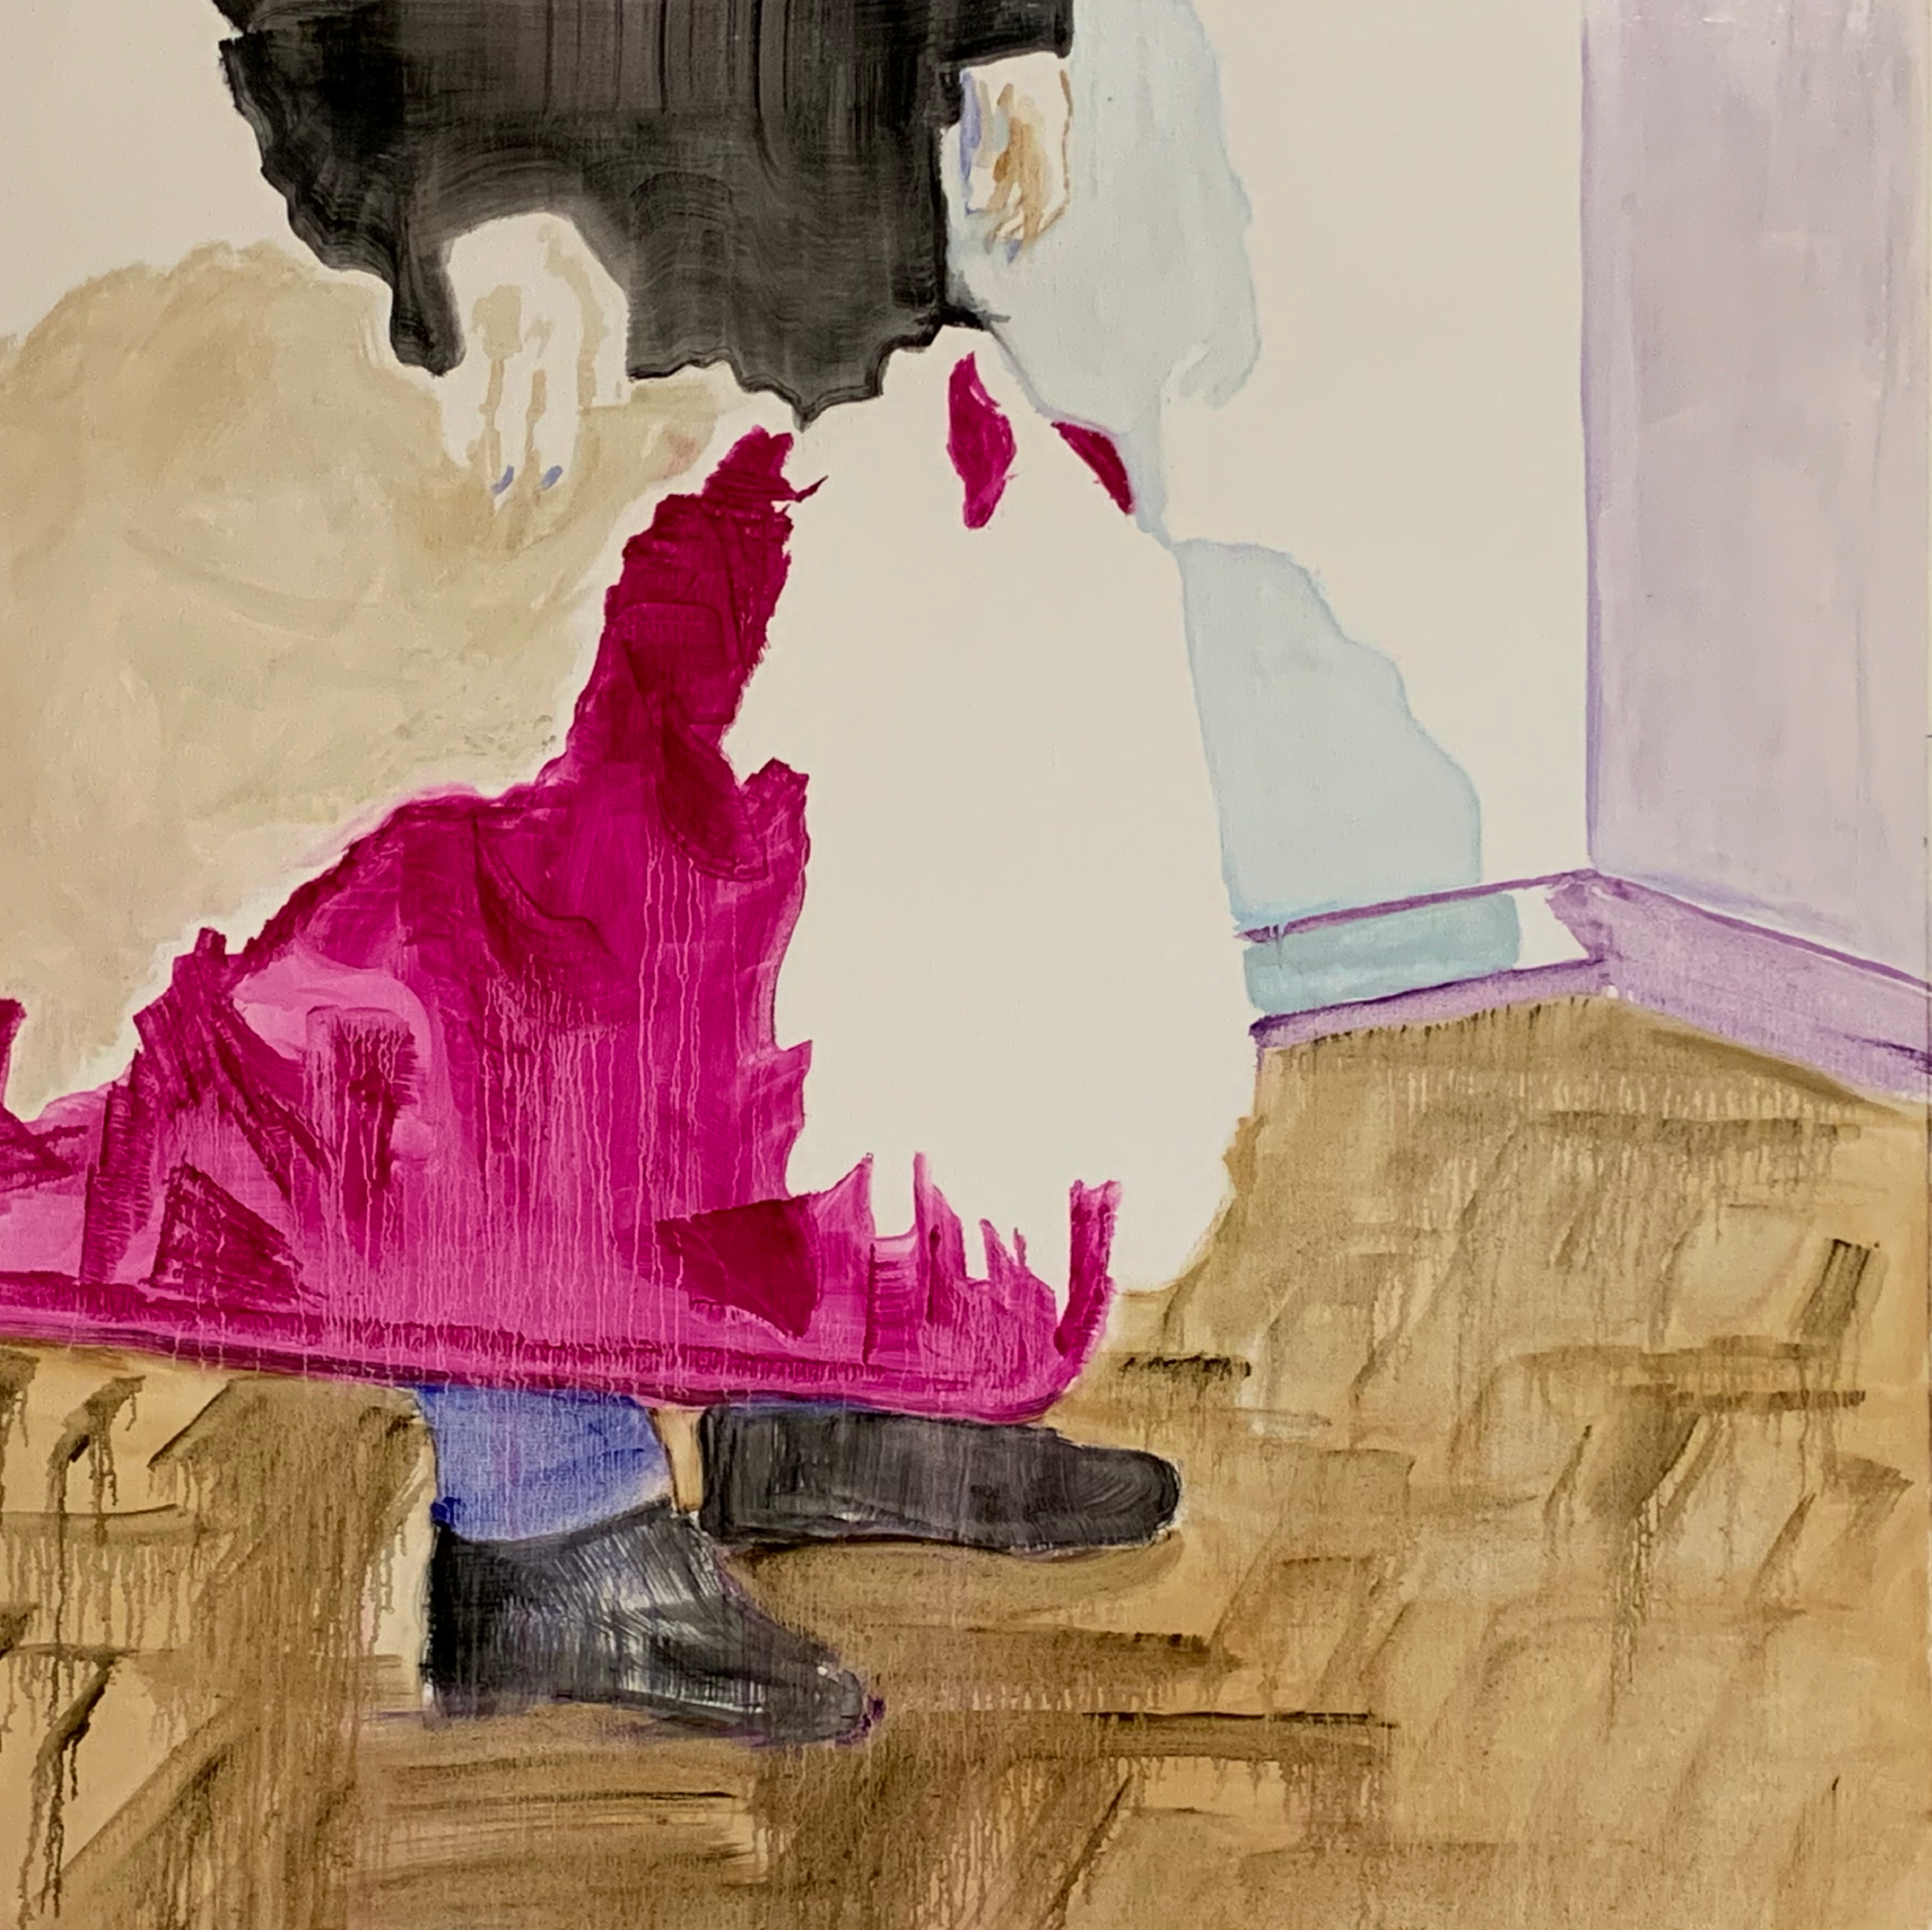
\includegraphics[height=2.49903in]{figuras/odette-carregando-mala-2021-esboco.pdf}
	\figurenote{\series{Me leva}. \oleolinho. \artsize{80x80}. Fonte: \archivef}
\end{minipage}\hfill
  \begin{minipage}{.45\linewidth}
	\caption{\artname{\odette}{Carregando a mala}{2021}}
	\includegraphics[height=2.49903in]{figuras/odette-carregando-mala-2021.pdf.compressed.pdf}
	\figurenote{\series{Me leva}. \oleolinho. \artsize{80x80}. Fonte: \archivef}
\end{minipage}
\end{figure}

A pintura se tornou mais fluida, mas mantendo sempre o interesse em
usar um impaste na finalização. No final de 2021, em viagem pelo
Brasil, me aventurei na linguagem tridimensional. Construí o meu
primeiro objeto instalativo, que se chama \emph{Por dois fios,} numa
alusão aos fios que nos ligam à terra. Construído com aramado de metal
e sobreposição de rendas têxteis, foi fotografado com uma iluminação de
estúdio e exposto virtualmente através do Instagram. Esta foi a última
mala que eu efetivamente criei.

\begin{figure}
  \flushright
  \begin{minipage}{3.28742in}
	\caption{\artname{\odette}{Por dois fios}{2021}}

  \includegraphics[width=2.7in]{figuras/odette-por-dois-fios-2021.pdf.compressed.pdf}
	\figurenote{\series{Me rendo}. Objeto instalativo. Dimensões variadas.
		Foto Adilson D'~Avilla. Fonte: \archivef}
\end{minipage}
\end{figure}

O Projeto \emph{Nem tudo é cor de Rosa} apresentou pinturas das malas
na exposição virtual \emph{paralela EIXO 2021.} A ideia era falar sobre
o cenário fantástico e inexplicável dos tempos de pandemia. Uma ideia
meio de sonho ou pesadelo. Em seguida, interessada em trabalhar em
pinturas que retratam uma atmosfera fantasiosa, iniciei uma série com
fundo verde em \emph{chroma} luminoso (na paleta \emph{viridian} e
\emph{phtalo green}). Escolhi a pintura \emph{O Balanço} (1767--1768),
de \emph{Fragonard} (1732--1806), ícone do movimento Rococó que se
iniciou no século~XVII\@. Este movimento se caracterizava por um
acúmulo de detalhes, e de muita frivolidade. Liberdade para sonhar. O
Rococó me fez pensar nos detalhes das rendas de minha coleção de
apliques usados nas costuras da minha mãe. O vestido esvoaçante e
detalhado da mocinha retomava o tema de tecidos que já havia explorado
alguns anos antes.

\begin{figure}[b]
	\caption{Estudo de elementos em colagem digital.}

	\includegraphics[width=2.79257in,height=2.09459in]{figuras/estudo-elementos-colagem-digital.pdf.compressed.pdf}
	\figurenote{Fonte: \archivef}
\end{figure}

Partindo da técnica de colagem, não a tradicional, mas digital,
realizei uma espécie de decupagem,\footnote{Decupagem in Priberam ---
	2.~\textins{Cinema, Televisão}~Divisão de um texto em cenas e planos,
	com escolhas e anotações técnicas e cênicas~para gravação ou filmagem.}
pintei um céu com um balanço em 3 posições, simulando o movimento de um
pêndulo. Embora já trabalhasse com pintura há muitos anos, esta foi a
primeira vez que experimentei a colagem, para pensar a composição de
elementos e narrativa dentro de um cenário.

\begin{figure}
  \begin{minipage}{.45\linewidth}
	\caption{Estudo com base em decupagem de elementos da colagem}

	\includegraphics[width=2.84478in,height=1.89189in]{figuras/estudo-decupagem-elementos-colagem.pdf.compressed.pdf}
	\figurenote{Fonte: \archivef}
\end{minipage}\hfill
\begin{minipage}{.45\linewidth}
  \caption{Estudo para projeção por exclusão de matizes \phantom{aaaaaaaaaaaaaaa}}
	\includegraphics[width=2.83748in,height=1.86486in]{figuras/estudo-projecao-exlusao-matizes.pdf.compressed.pdf}

	\figurenote{Fonte: \archivef}
\end{minipage}
\end{figure}

A mocinha do Fragonard ficou de fora desta pintura, porque não tinha
definida a forma como entraria no trabalho. Decidi então voltar a usar
o rosa (o mesmo da pintura \emph{Carregando a mala}) na imprimatura,
para fazer um céu. Escolhi como referência para esta pintura o trabalho
de Will Cotton (1965), que possuía corpos bem fantasiosos sobrepostos à
imagem de um céu. O título desta pintura ficou assim: \emph{No quintal
	da vovó tinha um balanço}.

\begin{figure}
\begin{minipage}{.6\linewidth}
	\caption{\artname{\odette}{No quintal da vovó tinha um balanço}{2021}}%
	\label{odette-quintal-vovo-tinha-balanco-2021}
	\includegraphics[width=3.38543in,height=2.229in]{figuras/odette-quintal-vovo-tinha-balanco-2021.pdf.compressed.pdf}
	\figurenote{\series{Movimento de câmera}. \oleolinho  \artsize{47x72x4}. Foto da autora}
\end{minipage}\hfill
\begin{minipage}{.3\linewidth}
	\caption{\artname{Will Cotton}{Fairy Floss}{2009--2010}}
	\includegraphics[height=2.229in]{figuras/cotton-fairy-floss.pdf.compressed.pdf}
	\figurenote{Fonte: \hiperlink{www.willcotton.com/paintings/2009.html}{Sítio de Will Cotton}}
\end{minipage}
\end{figure}

Experimentei formas distintas de pintar a mocinha, inclusive sobre
recortes em tecido, a fim de chegar a alguma possibilidade de inclusão
deste elemento na série do balanço. Por se tratar de uma figura humana
muito detalhada, me sentia pouco à vontade para jogá-la diretamente na
composição.

\pagebreak

A possibilidade de explorar o Movimento sequencial em repetição do
cinema me atraía, e assim nasceu a série \emph{Sapatinhos Voadores},
que se mescla com o projeto \emph{Balanço}. Fiz novos estudos através
da colagem, criando o díptico \emph{Elas levantam a saia e chutam},
onde recorto as figuras e pinto a óleo sobre tecido de algodão brocado.

\begin{figure}
  \flushright
\begin{minipage}{3.9in}
	\caption{\artname{\odette}{Elas levantam a saia e chutam}{2021}}
	\includegraphics[width=1.85432in,height=1.86598in]{figuras/odette-elas-levantam-saia-chutam-esquerda.pdf.compressed.pdf}
	\includegraphics[width=1.85903in,height=1.86339in]{figuras/odette-elas-levantam-saia-chutam-direita.pdf.compressed.pdf}
	\figurenote{\series{Sapatinhos voadores}. Colagem e Óleo sobre têxtil e linho. \artsize{15x30x3.5}. Foto da autora}
\end{minipage}
\end{figure}

O projeto atual, \emph{Olhar do cinema}, inicia logo após a realização
da pintura de um balanço, intitulada \emph{Memória em Inércia}, no qual
eu me inspiro no movimento do cinema, como uma espécie de metáfora
invertida.

\begin{figure}
	\caption{\artname{\odette}{Memória em
			inércia}{2021}}

	\includegraphics[width=1.85297in,height=2.81553in]{figuras/boudet-memoria-inercia-2021.pdf.compressed.pdf}
	\figurenote{\series{Movimento de câmera}. \oleolinho. \artsize{30x20x3.5}. Foto da autora}
\end{figure}

Tratando especificamente deste projeto, de suas cores e de frames de
filmes ícones da história do cinema, passo a descrever, a partir de
agora, as primeiras pinturas que se relacionam diretamente com esta
temática.

Os enquadramentos, as angulações propostas pelo posicionamento da
câmera de filmar sempre me atraíram. O ponto de vista, para
\textcite{jullier2009lendo} é tido como o parâmetro mais importante ao
nível do plano cinematográfico, e tem por princípio básico a
localização estratégica da câmera em relação ao cenário e seus
elementos estáticos e em movimento. Com relação ao espaço
tridimensional, o operador de câmera precisa fazer três escolhas
topográficas: o comprimento do eixo da objetiva (próximo ou distante,
close-up ou plano geral); na lateralidade (centralizado ou
descentralizado); e na verticalidade (câmera alta, câmera baixa, câmera
alta total, câmera baixa total, frontalidade e desenquadramento.
Entretanto, faz mais sentido flexibilizar estas posições de comprimento
do eixo durante a montagem, ou seja, no nível da sequência. Desta forma
tem-se o plano médio que apresenta o sujeito em sua unidade (seja ela
humana, animal, vaso de flores, automóvel), o close-up (ou plano
detalhe e grande plano em lusitano) e o plano geral, que insere o
sujeito em seu ambiente. Além disto cabe ressaltar a gíria\footnote{
	Linguagem usada por determinado grupo, geralmente incompreensível para
	quem não pertence ao grupo e que serve também como meio de realçar a
	sua especificidade. \textbf{\enquote{gíria}}, in Dicionário Priberam da
	Língua Portuguesa \textins{em linha}, 2008-2020,
	\hiperlink{https://dicionario.priberam.org/g\%25C3\%25ADria}{{https://dicionario.priberam.org/g\%C3\%ADria}}
	(consultado em 11 de janeiro de 2022).} do operador de câmera, que
preconiza um mínimo de \emph{ar}, em cima e embaixo dos sujeitos. Na
lateralidade existe a questão da centralização e descentralização, que
pode respeitar ou não a regra dos três terços, derivada da pintura. Na
verticalidade o eixo da objetiva aponta para o centro do sujeito, desce
na sua direção quando a câmera está alta ou sobe na direção do sujeito
quando a câmera está baixa. Quando o ângulo entre o plano do chão e o
eixo da objetiva se aproxima de 90º graus, fala-se em \emph{câmera alta
	total} ou \emph{câmera baixa total.} Por fim a frontalidade do
enquadramento e a busca pelo paralelismo no final de uma panorâmica
deveriam ser levados em conta pelo diretor de fotografia %
\parencite[22-28]{jullier2009lendo}.

Percebemos, pela sistematização destes autores, que muitas das decisões
de posicionamento da câmera nas captações de imagem, guardam uma
intimidade grande com as que o pintor, no seu relacionamento com a tela
precisa tomar. Nesta perspectiva, o olhar da câmera poderia substituir
o gesto do pintor. E aqui podemos falar sobre o posicionamento do
pintor diante da tela. O corpo se movimenta, buscando a melhor forma de
iniciar o movimento, para aplicar o carvão, o pigmento, a tinta ou
qualquer outro tipo de matéria que se possa tratar na pintura. Uma
dança acontece entre a imagem mental e o impulso que alcança o objeto.
Aproximações e afastamentos, necessários à visualização do todo e do
pormenor da composição também acontecem, ora mais despojadas, ora mais
intimistas, nas tentativas de ensaio, erro, tirar, pôr, riscar, afagar,
bater, secar e deixar escorrer. Seja com a tela na forma vertical,
horizontal à moda de \emph{Pollock}, seja nos planejamentos de direção
cromática, dentro do quadro. As marcações, medidas que os fotógrafos de
câmera fazem antes do início do filme, se equivalem aos esboços que se
utilizam tanto de linhas feitas com carvão, fita-crepe, pincéis, giz, e
como estratégia cada vez mais usada por pintores contemporâneos, como o
uso do projetor.

\begin{figure}
  \begin{minipage}[b]{.475\linewidth}
	\caption{\artname{\odette}{Eu quero ir}{2020}}%
	\label{boudet-eu-quero-ir-2020}

	\includegraphics[width=.8\linewidth]{figuras/boudet-eu-queri-ir-2020.pdf.compressed.pdf}
	\figurenote{\series{Me leva}. \oleolinho. \artsize{30x20x4}. Foto da autora.}
\end{minipage}\hfill
\begin{minipage}[b]{.475\linewidth}
	\caption{\artname{\odette}{Contre plongée}{2020}}%
	\label{boudet-contre-plogee-2020}

	\includegraphics[width=.8\linewidth]{figuras/boudet-contre-plogee2020.pdf.compressed.pdf}
	\figurenote{\series{Me leva}. \oleolinho. \artsize{20x20x4}. Foto da autora}
\end{minipage}
\end{figure}

O \emph{plongée}, que significa mergulho, foi pensado para relacionar
dois trabalhos: \emph{Eu quero ir, 2020}, e \emph{Contre-plongée,
2020} (\cref{boudet-eu-quero-ir-2020,boudet-contre-plogee-2020}). O mergulho que a câmera do cinema dá ao enquadrar uma
determinada cena e a ideia de campo/contracampo inspiraram a
apresentação destas duas pinturas \emph{que se olham}. A mala se coloca
em \emph{contra-plongée} e lança um olhar para a fechadura da porta.

Quando realizei a pintura \emph{Na casa da vovó tinha um balanço}
(\cref{odette-quintal-vovo-tinha-balanco-2021}) minha intenção era
refletir sobre o Movimento de ir e vir, como em um pêndulo. Muito tempo
depois, analisando as pinturas \emph{Eu quero ir}
(\cref{boudet-eu-quero-ir-2020}) e \emph{Contre-plongée}
(\cref{boudet-contre-plogee-2020}), compreendi a relação entre uma
imagem afetiva e o ponto de vista habituado à intermediação de uma
câmera. Eu pesquiso na pintura recortes na composição da imagem
fotográfica e a intermediação de uma câmera muitas vezes atravessa o
pensamento e o gesto. Compreender o mundo para mim é instaurar uma
imagem. Aquela que mesmo sem sabermos de que parte da memória vem,
precisa ser colocada diante de nós. Foi assim com o projeto Balanço.
Ele veio e só depois de algum tempo eu o enxerguei lá, em um
enquadramento plongée. \emph{Era o balanço no quintal da vovó, visto de
	cima da minha varanda.}

Criar um \emph{storyboard}, por meio da pintura também era e ainda é um
objetivo. No entanto, muito antes de construir uma narrativa, a
finalidade maior sempre foi experimentar técnicas e processos na
pintura. Realizei as pinturas \emph{Under the bed, 2021} (\cref{under-the-bed}) e
\emph{Rolamento suspenso, 2021} (\cref{rolamento-suspenso}) e criei a série \emph{Movimento de
	câmera}, imaginando a mala se movimentando e saindo debaixo da cama.
Dei seguimento a este grupo de trabalhos com a pintura \emph{Retrato na
parede, 2021} (\cref{retrato-na-parede}), onde as rodinhas da mala criam uma sombra sobre um fundo
branco.

A série intitulada \emph{Movimento de câmera} veio ao encontro dos
primeiros estudos para o Projeto \enquote{Olhar do cinema}. Foi a
partir desta série que apliquei uma metodologia que parte da
identificação dos principais interesses do artista, por meio de escolha
aleatória de figuras, paletas e padrões, caminhando para ideias de
esboços e trabalhos finalizados, que se desdobram em séries e projetos.

\newpage

\begin{figure}
  \begin{minipage}[b]{.3\linewidth}
  \caption{\artname{\odette}{Rolamento suspenso}{2021}.}\label{rolamento-suspenso}

  \includegraphics[width =.88\linewidth]{figuras/boudet-rolamento-suspenso-20201.pdf.compressed.pdf}
	\figurenote{\series{Movimento de câmera}. \oleolinho. \artsize{37.5x37.5x4}. \\ Foto da autora.}
\end{minipage}\hfill
\begin{minipage}[b]{.3\linewidth}
  \caption{\artname{\odette}{Under the bed}{2021}.}\label{under-the-bed}
	\includegraphics[width = \linewidth]{figuras/boudet-under-the-bed-2021.pdf.compressed.pdf}
	\figurenote{\series{Movimento de câmera}. \oleolinho. \artsize{57.5x82x4}. \\ Foto da autora.}
\end{minipage}\hfill
\begin{minipage}[b]{.25\linewidth}
  \caption{\artname{\odette}{Retrato na parede}{2021}}\label{retrato-na-parede}

	\includegraphics[width=.6\linewidth]{figuras/boudet-retrat-na-parede-2021.pdf.compressed.pdf}
	\figurenote{\series{Movimento de câmera}. \oleolinho. \artsize{20x20x4}. \\ Foto da autora}
\end{minipage}
\end{figure}

\section{Definindo o tema}\label{definindo-o-tema}

Coletar imagens que nos sensibilizam, de forma aleatória pode ajudar a
quem não tem certezas sobre o assunto que quer tratar. A criação de um
banco de imagens e recolha constante de fontes, pode ser um hábito no
processo criativo de um pintor, que o ajudará muitas vezes a escolher o
quê, o porquê e o como na elaboração de um projeto artístico. A partir
desta coleta inicial, é possível identificar os conceitos de maior
interesse através de sua recorrência.

No processo de criação do projeto \emph{Olhar do Cinema}, observei a
minha produção de pintura desde o seu início, passando pelas decisões
de trabalhar com pintura a óleo e figurativa, até chegar ao ponto em
que me encontro, visando a execução de um projeto que se relacione com
o tema desta dissertação. A produção de pintura já tinha uma longa
estrada e são muitas as imagens que carrego nas costas. O \emph{Atlas
	Mnemosyne} de Aby Warburg me inspirava e a Mala que Walter Benjamin
deixou com seus escritos inacabados, também. Como organizar e
selecionar tantas informações e interesses? Optei por separar as
referências em pastas no aplicativo Pinterest (\cref{o-esbouxe7o-o-quadro-o-formato-e-o-projetor})
, visando escolher um
ponto de partida. A motivação inicial de querer saber como se constrói
uma imagem através do olhar do cinema deu nome às pastas:
\emph{movimento, olhar, humano e cenário.}

\begin{figure}
	\caption{Capturas de ecrã. }

	\includegraphics[width=2.33526in,height=3.08547in]{figuras/captura-ecra.pdf.compressed.pdf}
	\figurenote{Fonte: página do Pinterest da autora}
\end{figure}

\section{O esboço, o quadro, o formato e o projetor}%
\label{o-esbouxe7o-o-quadro-o-formato-e-o-projetor}

\paragraph{O esboço} Após definir os primeiros temas, o segundo passo para a criação do
projeto seria a realização de esboços, um hábito que eu não tinha, pois
sempre parti diretamente para a realização do trabalho final. Para esta
etapa seria necessário selecionar referências e decidir o formato que
iria trabalhar: a janela e o quadro, onde tudo começa.

\paragraph{O quadro} Levando em conta estes aspectos abordados no \cref{cap1-contexto-relacao-cinema-pintura}, ao tratar das
teorias relacionadas a espaço, concluímos que um dos pontos de
interseção mais claros entre o cinema e a pintura certamente é o
\emph{quadro}. As relações com o quadro, seus limites e o desejo de
transformá-lo em uma janela para o mundo real é objeto do texto de
Jacques Aumont sobre o quarto de Van Gogh. Esta janela hoje tem um
nome: a câmera de um celular e seus muitos aplicativos. Outro exemplo
sobre o quadro é o \emph{assunto} da pintura da Lúcia Laguna, que se
encontra do outro lado da Janela. Hitchcock faz uma verdadeira ode ao
quadro em seu filme \emph{A janela indiscreta (1954)} e Woody Allen
leva seu personagem em \emph{A Rosa púrpura do Cairo (1985)}
literalmente para dentro do espaço narrativo do filme.

\paragraph{O formato} Ao iniciar uma pintura, nos moldes tradicionais sobre um suporte em
tela, painel, é preciso contar com estes limites e decidir o seu
formato. Nosso objetivo de criar um projeto artístico de
pintura sobre tela precisou refletir, logo no início, sobre este
aspecto.

Por muito tempo, no meu caso, esta decisão se relacionava diretamente
com a imagem fotográfica de referência e com a estratégia compositiva
dos seus elementos, que em geral eram posicionados por meio da análise
de \emph{golden lines}.

Como já mencionado no início deste capítulo, sobre a Série
\emph{Penumbra}, o meu processo se iniciava com um ensaio de
fotografias que eram projetadas sobre a tela ou linho grampeados na
parede, com a finalidade de realizar o esboço através de pintura
indireta. As reflexões sobre a composição da imagem começam, já nos
recortes da fotografia que será projetada. Este é um processo que uso
há muitos anos e as decisões finais sobre o formato em geral ocorrem
neste momento inicial de projeção.

A pandemia direcionou nossas exposições para o espaço virtual. Em
consequência, optei por unificar o formato de todas as obras para o
quadrado. Dois motivos me levaram a esta decisão: a ideia da formação
da imagem audiovisual em pixels; e os formatos de aplicativos nas redes
de compartilhamento como Instagram, para ecrãs dos celulares\slash
telemóveis.

\paragraph{O projetor} Com o formato definido, é preciso ainda checar se o arquivo da imagem
tem a sua extensão apropriada para uso no projetor, que de preferência
deve ter mais de 3000 lumens. Neste momento começa a melhor parte.
Nosso corpo se interpõe entre a luz do projetor e a tela que será
abordada por instrumentos da pintura. A experiência de estar em uma
sala de cinema é trazida de volta e neste momento, é possível abandonar
um pouco a rigidez de todo um planejamento prévio. O mundo do cinema e
o da pintura se encontram de certa forma nesta hora.

A marcação por meio de projetores para iniciar um trabalho pictórico,
método muitas vezes usado por pintores contemporâneos, vem se somar aos
tradicionais esboços com os modelos vivos e técnicas de ampliação de
desenho. Podemos afirmar que esta parte do meu processo criativo
acontece de maneira indireta, onde os modelos do mundo real já sofreram
um tratamento por outros meios de representação da imagem, no caso a
fotografia e o cinema.

\section{O desenvolvimento do projeto}%
\label{o-desenvolvimento-do-projeto}

Retomando a questão do tema, elaborei alguns esboços em ateliê para
representar as imagens coletadas, com ideias de movimento, olhar,
humano e cenário. Ícones dos primeiros filmes: o trem dos irmãos
Lumière e \emph{Viagem à Lua} de Méliès foram as imagens escolhidas
para os primeiros esboços, com a finalidade de \emph{aquecer os
	pincéis} e de realizar testes de cor, moldes, suportes e formatos. Para
estes testes, agreguei referências de processos de alguns pintores como
Gerhard Richter.

\begin{figure}
  \begin{minipage}[t]{.4\linewidth}
    \caption{Esboço Série Olhar do Cinema. Teste Phtalo blue. \phantom{aaaaaaaaaaaaaaaaaaaaaaaaaaaa}}
	\includegraphics[height=1.30866in]{figuras/boudet-esboco-olhar-do-cinema.pdf.compressed.pdf}
	\figurenote{Artista de referência Gerhard Richter. \oleo. \artsize{20x20}. Foto da autora.}
\end{minipage}\hfill
\begin{minipage}[t]{.4\linewidth}
	\caption{Teste de preto Cromático
		Phtalo Blue e Quinacridona Rose --- \artname{\odette}{Estação Lumière I}{2022}.}

	\includegraphics[height=1.30866in]{figuras/boudet-test-preto-cromatico-2022.pdf.compressed.pdf}
  \figurenote{\series{Espaço no ecrã} \oleo. \artsize{20 x 20}. Foto da autora \phantom{aaaaaaaaaaaaaaaaaaa}}
\end{minipage}
\end{figure}

Alguns destes esboços se transformavam em trabalhos finalizados.

\begin{figure}
  \begin{minipage}[t]{.3\linewidth}
	\caption{Molde de máscara vazada em acetato}

	\includegraphics[height=1.30833in]{figuras/molde-mascara-vazada-acetato.pdf.compressed.pdf}
\end{minipage}
\begin{minipage}[t]{.3\linewidth}
	\caption{Esboço fluido do trem sobre molde blocado.}

	\includegraphics[height=1.30833in]{figuras/esboco-fluido-trem-sobre-molde-blocado.pdf.compressed.pdf}
  \figurenote{Proporção \emph{medium} 1 linhaça para 5 de \emph{white spirit}}
\end{minipage}
  \begin{minipage}[t]{.3\linewidth}
	\caption{Esboço de \enquote{\emph{blurrr}} em máscara vazada.}

	\includegraphics[height=1.30831in]{figuras/esboco-blurrr.pdf.compressed.pdf}
\end{minipage}
\end{figure}


\begin{figure}
\begin{minipage}{.4\linewidth}
	\caption{Processo de William Kentridge --- 7 fragmentos para Georges
		Meliés.}

	\includegraphics[height=1.98507in]{figuras/kentridge-7-fragmentos-georges-melies.pdf.compressed.pdf}
	\figurenote{Captura de ecrã. Fonte: \hiperlink{http:\\www.kentridge.studio/projects}{Kentridge Studio}}
\end{minipage}\hfill
\begin{minipage}{.4\linewidth}
  \caption{\artname{\odette}{Cena Méliès I}{2022} \phantom{aaaaaaaaaaaa}}

	\includegraphics[height=1.98507in]{figuras/boudet-cena-melies.pdf.compressed.pdf}
	\figurenote{\series{Fora de Campo}. Tratamento com restos de tinta da paleta. Foto da autora}
\end{minipage}
\end{figure}


\paragraph{\emph{Frames} de filmes} Com o objetivo de aproximar a experiência do cinema à da
pintura, explorei alguns assuntos por meio de \emph{frames} de filmes.
Em consequência, avaliei que um dos eixos, o Olhar, abrangia os demais.
Iniciou-se então uma reconfiguração nos títulos das series dos esboços
e posteriormente das obras em finalização. O termo \emph{olhar} ou
\emph{olhar do cinema} transformou-se na matriz principal para os
esboços subsequentes, que subdividiram em três: \emph{movimento, humano
	em frames e cenário no cinema/espaço profundo}. Este Projeto que também
dava nome à série de esboços \emph{Olhar do cinema}, passou a se
desenvolver paralelamente ao Projeto \emph{O balanço}, que também fazia
referência ao conceito de movimento, só de uma outra forma. Este novo
viés da pesquisa é sobre a construção de uma pintura atravessada pelo
olhar de uma câmera em movimento.

Como já descrito no \cref{cap2-impacto-evolucao-otica}, a palavra
movimento se apresenta sempre que tentamos associar a imagem na pintura
figurativa à do cinema: \emph{impressão de movimento}. A experiência
com o objeto mala em pintura, além de contemplar a questão do movimento
e deslocamento, de um ponto de vista metafórico, apontava também para
um terceiro problema, que é o da \emph{memória do artista}. Além do ir
e vir das imagens mentais que ora estão mais próximas, ora mais
distantes, remete à prática de olhar de perto e olhar de longe comum a
muitos artistas durante o ato de pintar.

\begin{figure}
  \caption{Esboço referência Homem com uma câmera de Dziga Vertov}\label{esboco-dziga-vertov}

\includegraphics[width=1.65432in,height=1.61402in]{figuras/esboco-referencia-homem-camera.pdf.compressed.pdf}
\end{figure}

As pesquisas relacionadas ao \emph{objeto} na pintura, que antecederam
o início deste mestrado, tinham origem nos planos próximos viabilizados
pela câmera de filmar. Da mesma forma, as possibilidades de
enquadramentos e ângulos utilizados nas fotografias de referência
ditavam as escolhas de cortes para posicionamento destes \emph{objetos}
na tela da pintura. As temáticas se sucederam, mas a ideia continua
sendo a mesma, uma preocupação em criar um \emph{cenário} com base na
imagem construída pelas lentes de uma câmera. Neste sentido, encontrei
na estética do \emph{Cinema olho} e do filme \emph{O Homem com uma
câmera} (\cref{esboco-dziga-vertov}), de Dziga Vertov uma referência importante. A série
\emph{Humano} se materializou por meio de um esboço inspirado neste
filme. O esboço se transformou em trabalho final.


Com \emph{Hitchcock}, comecei a unir ideias importantes como o
posicionamento da câmera, o fora de campo e a progressão visual de
Block (uma coisa que se transforma em outra) e o \emph{fora de campo}.
Percebi que a tônica sobre a questão do espaço, invadiu a pintura. Foi
preciso revisar os conceitos das séries dentro do projeto expositivo.
Mas enquanto não aprofundava termos da narrativa visual como espaço
plano, espaço profundo e espaço fora de campo, por meio de novas
sequências de trabalhos, as pinturas \emph{Vertigo I, II e III}
permaneceram na série \emph{Humano em frames}.

\begin{figure}
  \begin{minipage}{.3\linewidth}
  \caption{\artname{\odette}{Vertigo I}{2022} \phantom{aaaaaaa}}

	\includegraphics[width=1.77199in,height=1.77679in]{figuras/boudet-vertigo-I-2022.pdf.compressed.pdf}
	\figurenote{\series{Humano em frames}. \oleolinho. \artsize{40x40x3.5}}
\end{minipage}\hfill
\begin{minipage}{.3\linewidth}
	\caption{\artname{\odette}{Vertigo II}{2022}}

	\includegraphics[width=1.8125in,height=1.77709in]{figuras/boudet-vertigo-II-2022.pdf.compressed.pdf}
	\figurenote{\series{Humano em frames}. \oleolinho. \artsize{40x40x3.5}}
\end{minipage}\hfill
\begin{minipage}{.3\linewidth}
	\caption{\artname{\odette}{Vertigo III}{2022}}

	\includegraphics[width=1.81045in,height=1.76806in]{figuras/boudet-vertigo-III-2022.pdf.compressed.pdf}
	\figurenote{\series{Humano em frames}. \oleolinho. \artsize{40x40x3.5}}
\end{minipage}
\end{figure}

O \emph{personagem} da mala fechada, frequentemente o único elemento da
cena, serviu ao objetivo de representar possíveis significados poéticos
e metafóricos com diferentes abordagens. Agora é preciso afinar o
projeto expositivo a linhas de pensamento voltadas para estruturar a
narrativa visual do filme, tal qual orienta Block.

As ramificações das teias deste universo se expandem e contraem, e
\textcite{deleuze2004imagem} traz a ideia das imagens rarefeitas e
esvaziadas.

\begin{displaycquote}[22-23]{deleuze2004imagem}[.]
	\textelp{} imagens rarefeitas são produzidas, seja quando toda a tônica é
	posta num só objeto (em Hitchcock, o copo de leite iluminado do
	interior, em \emph{Suspicion}\footnote{Filme Suspeita (1941)}, a brasa
	do cigarro no retângulo negro da janela, em \emph{Rear
		Window}\footnote{Filme Janela indiscreta (1954)}), seja quando o
	conjunto está vazio de certos subconjuntos (as paisagens desertas de
	Antonioni, os interiores esvaziados de Ozu). O máximo de rarefação
	parece atingido com o conjunto vazio, quando o ecrã aparece todo preto
	ou todo branco. Hitchcock dá um exemplo em \emph{Spellbound}\footnote{Filme
		A Casa Encantada (1945)}, quando um outro copo de leite invade o ecrā,
	deixando apenas uma imagem branca vazia. Mas, das duas vezes, rarefação
	ou saturação, o quadro ensina-nos assim como a imagem não nos dá apenas
	a ver. Ela é tao legível como visível
\end{displaycquote}

Com isto, intuí que a forma figurativa deveria dar um passo atrás e
sair de campo, oferecendo espaço para \emph{conceitos}. No
\emph{Capítulo Quadro e Plano, Enquadramento e Décupage}, ele segue:

\begin{displaycquote}[25]{deleuze2004imagem}[.]
	\textelp{} É sobre o \emph{principal e o secundário}\ldots\ O quadro é, pois,
	inseparável de duas tendências, à saturação ou à rarefação. Sobretudo o
	grande ecrã e a \emph{profundidade de campo} permitiram multiplicar os
	dados independentes ao ponto que uma cena secundária aparece na frente,
	enquanto o principal se passa no fundo (Wyler), ou que já não se pode
	fazer uma diferença entre o principal e o secundário (Altman)
\end{displaycquote}

Criei o título da série \emph{Espaço no ecrã}, que abrigou o termo
\emph{profundidade de campo}. Com a possibilidade de trabalhar o espaço
arquitetônico ainda rarefeito, sinalizando aos poucos o espaço
profundo, apto a receber alguns elementos para compor uma narrativa.
Desta forma, me conectei a conceitos estéticos cinematográficos de Ozu
(1903--1963). Segundo \textcite{dias2016riso}, a essência do cinema
utilizada por Ozu, explica a frequente qualificação de seus filmes
contemplativos como \emph{poéticos}. Para ele, a estética das imagens
de Ozu são o resultado de três fatores de ordem formal.

\begin{displaycquote}[136-137]{dias2016riso}[.]
	Em primeiro lugar, o rigoroso sentido de composição de cada plano,
	\textelp{} o geometrismo dessa composição, dos enquadramentos dos planos,
	de interiores e de exteriores \textelp{}. Toda uma \emph{picturalidade} da
	cine-imagem, toda uma infinita aproximação \emph{ozuiana} do cinema e da
	pintura, mas para assim afirmar a infinita distância entre os dois
	tipos, pictórico e cinematográfico, de imagens
\end{displaycquote}

A câmera quase sempre fixa e seu posicionamento oblíquo, evidenciaria
um efeito de profundidade de campo, e um distanciamento contemplativo,
aproximando assim a percepção do contemplador de pintura à do
espectador do filme. \enquote{De resto, o próprio Ozu declarava que o
	movimento é um atributo da câmera, mas \emph{não} do cinema\ldots\ O
	cinema de Ozu é, nisso, perfeitamente clássico, um cinema de montagem}
\parencite[138]{dias2016riso}. Os planos fixos, estáticos, por si só já
contam a história da pintura e do filme.

Pela observação dos aspectos analisados neste Capítulo, conclui-se que
o desenvolvimento do projeto deve muito à criação de uma metodologia
para registrar as ramificações relacionadas à temática. Neste sentido,
foi importante trazer as investigações sobre o movimento metafórico das
figuras \emph{mala} e \emph{balanço}, com as quais também realizei
experimentos audiovisuais. Além disto, a revisão bibliográfica de
teorias do cinema durante a dissertação, abriu possibilidades de
abordar conceitos como o do espaço profundo, espaço plano, progressão
visual, princípio de afinidade e contraste, rarefação e saturação, como
base para de projetos pictóricos. Até o presente momento, os títulos
das séries e pinturas do projeto \emph{Olhar do cinema} se encontram
com a configuração abaixo:

\begin{enumerate}
	\item Série Consequências

    \begin{enumerate}[topsep = 0pt]
		      \def\labelenumi{\arabic{enumi}.}
		      \item Plongé e contre-plongée
		      \item Storyboard
		      \item Progressão visual
		      \item Princípio de afinidade e contraste
	      \end{enumerate}

	\item Série Espaço no ecrã

    \begin{enumerate}[topsep = 0pt]
		      \def\labelenumii{\arabic{enumii}.}
		      \item Espaço profundo e espaço plano
		      \item Profundidade de campo
		      \item Rarefação e saturação
	      \end{enumerate}
	\item Série Humano em frames

    \begin{enumerate}[topsep = 0pt]
		      \def\labelenumii{\arabic{enumii}.}
		      \item Dziga Vertov
		      \item Vertigo
		      \item Victor Erice
		      \item Truffaut
	      \end{enumerate}
	\item Série Cenário Fora de campo

    \begin{enumerate}[topsep = 0pt]
		      \def\labelenumii{\arabic{enumii}.}
		      \item Cena Méliès
		      \item Atlântico norte I e II
		      \item Atlântico sul I
	      \end{enumerate}
\end{enumerate}

\section{A cor}\label{a-cor}

Finalizo este capítulo descrevendo meu processo decisório pessoal
relacionado à cor. Os estudos de \emph{Notan}\footnote{Notan --
	definição. - www.virtualartacademy.com/notan/} ajudaram a pensar a
distribuição dos valores de claros e escuros na pintura, independente
dos matizes. A palavra japonesa \emph{Notan} significa \emph{escuro,
	claro}, derivada de \emph{Nong} (expresso, forte concentrado) e
\emph{Dan} (fraco, aguado). Refere-se à quantidade de luz refletida, ou
à massa de tons de diferentes valores. A técnica do \emph{Notan} me foi
apresentada nas aulas de pintura da Escola de Belas Artes da UFRJ em
2016, pela professora e artista Monique Queiroz (e serviu de apoio para
as primeiras pinturas no processo indireto, que realizei naquele
período. O \emph{Notan} como ferramenta de estudo da composição é
bastante útil para trabalhar com formas mais orgânicas, bem como para
realizar as primeiras camadas do processo indireto no estabelecimento
de valores.

Atualmente, antes de projetadas, as imagens de referência, são editadas
para excluir os matizes, permanecendo quase que somente o preto, o
branco e poucas tonalidades de cinza. Este processo é realizado
especialmente para os trabalhos em camadas e foi desencadeado pelos
estudos de Notan.

Mas como lidar com a cor no cinema e na pintura?

Embora a percepção das cores na pintura e no cinema pareça semelhante,
existem algumas diferenças a serem consideradas. O resultado da cor que
se vê em uma tela de pintura provém de uma luz refletida que atravessa
pigmentos e tinta. Já a luz que proporciona os diferentes matizes
percebidos em um ecrã de cinema, de celular ou de outros dispositivos
digitais é uma luz emitida e nos objetos eletrônicos são formadas por
adição. O sistema CMYK se baseia na pigmentação de \emph{Cyan, Magenta,
	Yellow e Black}. Neste sistema, objetos físicos como as telas de
pintura, as cores são reproduzidas através da subtração. Já no sistema
RGB, a luz é adicionada com níveis de cor desejados, formado pelas
cores \emph{Red, Green and Blue.}

Esta diferença pode se tornar um grande problema para os pintores mais
detalhistas, que trabalham com hiper-realismo, e para artistas gráficos
que dependem de uma alta precisão na reprodução das cores para produtos
impressos. No entanto sabemos que além do componente físico relacionado
à luz ambiente, sempre existirá uma diferença na percepção das cores de
acordo com o olhar do observador.

Existem muitos esquemas e teorias da cor à nossa disposição, que nem
sempre são suficientes para resolver o problema da articulação de
valores, matizes e cromas de forma a simplificar o trabalho do pintor.
A decisão sobre como escolher uma paleta para uma pintura, série ou
projeto pode se tornar algo bastante complexo. Por algum tempo utilizei
a teoria do \emph{Balão Cromático} (mencionado no Capítulo II) e dos
\emph{Contrastes} de Itten. Depois de muito pesquisar sobre os diversos
sistemas, esquemas e acordes de cor, ao longo da história da pintura,
adotei o quadro abaixo, disponibilizado pelo pintor Florence
Farges\emph{.} Em seus cursos de pintura on-line\footnote{Florent
	Farges www.florentfarges.com/the-art-and-practice-of-color/},
simplifica bastante para os artistas o modo como lidar com a matéria
das tintas e da cor.

\begin{figure}
	\caption{Teoria das Cores para artistas.}

	\includegraphics[width=4.7094in,height=2.64897in]{figuras/color-theory-for-artists.pdf.compressed.pdf}
	\figurenote{Fonte: \hiperlink{www.florentfarges.com/wp-content/uploads/2021/12/Color-Theory-for-Artists-Color-Wheel-System-1.pdf}{Florent Farges}}
\end{figure}

A professora de pintura \parencite{sabino2015pintura} revê a proposta de seu primeiro livro de
2000, já referenciado nesta dissertação, na forma abaixo:

\begin{displaycquote}[33]{sabino2015pintura}[.]
	o cerne da pintura poderia subsistir não na sua especificidade como
	médio ou na sua objetualidade, mas em algo mais imaterial, o que
	comparei a uma espécie de \enquote{configuração do olhar} que, antes da própria
	imagem do mundo e perante esta, fosse ela qual fosse, poderia atribuir a
	qualquer objeto visível características pictóricas e, assim, torná-lo em
	pintura ou, melhor ainda, fazer nele \enquote{acontecer} pintura
\end{displaycquote}

Após quinze anos da publicação de seu primeiro livro, ela declara
faltar-lhe algo mais fiável fisicamente, como a tinta.

Concluo que, por compartilhar desta visão pessoal de Isabel Sabino,
direcionei esta investigação no sentido de realizar uma pintura por
meio de estruturas visuais relacionadas ao cinema, e não o caminho
inverso. Acredito que não há nada mais importante para o ofício de um
pintor do que lidar com a fisicalidade da cor. Entretanto, o
encantamento com o mundo da tela preconizado por Hitchcock, no
\emph{voyeurismo} de \emph{A janela indiscreta (1954)}, e por com
milhares de narrativas fílmicas acumuladas ao longo da história do
cinema, me motiva a continuar buscando formas de conjugar estas duas
paixões. Paixões com as quais viajo não só para trás no tempo, à
procura de ensinamentos como os de \emph{Sargent} e \emph{Sorolla,} mas
também em busca de imaginar o futuro. Para mim, enquanto artista, é
fundamental estar atualizada com as novas tecnologias. E o mundo do
cinema e audiovisual me proporciona isto.

Hoje tenho consciência de que a cor saturada, e luminosa, derivada das
tintas a óleo transparentes que adotei depois de uma busca intensa,
passando pelo impaste opaco, traduz a visão e o sentimento de uma
imigrante dos trópicos. As escolhas técnicas que um pintor faz falam
muito da sua vida pessoal e da forma como se relaciona com seu mundo
contemporâneo. E isto vai se tornando cada vez mais claro ao longo de
sua trajetória. Concluo este capítulo com a certeza de que dentro da
minha mala, seja ela de pintura, de memórias ou afetos, sempre haverá
espaço para muitas histórias, contadas pela cor-luz emitida pelo
projetor, onde tanto gosto de mergulhar.


{
  \backmatter

  \chapter{Considerações Finais}%
\label{consideracoes}

Chega a hora de conciliar imagens e palavras a um ponto final. Rever o
percurso desta investigação desde quando decidi abraçar a causa da
pintura e me debruçar sobre inquietações de ordem pessoal, relacionadas
a duas artes bidimensionais: cinema e pintura. A escrita acadêmica,
para artistas, encontra temas de interesse não só ligados a questões de
ordem teórica sobre as humanidades, mas que com frequência se
entrelaçam ao seu trabalho prático.

Ao buscar responder à pergunta sobre como a tela branca pode ser
abordada como forma de expressão pessoal, cujo principal interesse eram
teorias de narrativa visual cinematográfica, trilhei um caminho que
passou pela revisão histórica das primeiras teorias da imagem em
movimento, já muito ligadas à história da pintura da época. Encontramos
a contextualização sobre o cinema em Xavier, 1983, que define a
estrutura e organização do filme como imagem e som \emph{organizados de
	um certo modo}. A \emph{impressão de realidade} é a tônica de um cinema
ficcional que, segundo ele, pouco mudou em seus princípios, no período
entre 1916 e 1980. Analisamos as relações do cinema com vanguardas
europeias em movimentos como o Impressionismo, Futurismo,
Expressionismo e Dadaísmo.

Cinema e pintura foram os dois campos pesquisados, cuja motivação se
iniciou nos anos 1980 com a experiência da câmera de filmar Super 8,
durante minha graduação em cinema, passando pelos estudos de pintura na
EAV e EBA, até chegar neste mestrado. Considerei a necessidade de
atualizar o referencial teórico, escolhendo autores ainda atuantes nas
academias, como Jacques Aumont, André Gardies e Delfim Sardo para
compor a perspectiva da investigação, que se firmou com o argumento de
Eric Rohmer de que o cinema é, acima de tudo, a arte do espaço. Com a
\emph{companhia} e o auxílio de historiadores da arte, teóricos,
curadores e pintores, realizei uma revisão bibliográfica
teórico/prática, a fim de responder três das minhas principais
indagações:

\begin{itemize}
	\item Qual a possibilidade de se utilizar o olhar característico do cinema,
	      no método processual da construção de uma pintura?

	\item Como se movimentam os olhos dos espectadores diante de uma pintura?

	\item Como é feita a seleção, pelos pintores, das referências que apoiarão
	      seus projetos?
\end{itemize}

Para tal finalidade, retomei as teorias de Jacques Aumont sobre
representação, espaço e quadro, relacionadas à produção de atmosferas
realistas no cinema. O texto de Aumont nos leva a confirmar a primeira
característica do olhar do cinema, que também diz respeito à pintura: o
quadro. 

Levando em conta estes aspectos, podemos dizer que questões
sobre a representação do espaço no quadro, seja na pintura à época de
Leonardo, seja no estilo centralizado \emph{hollywoodiano}, que reproduzia
técnicas antigas de centro de simetria, permanecem atuais, ainda que
tenhamos novas formas de visualização como IMAX, 3D, entre outras, que
se distanciam da noção convencional de ecrã no cinema e quadro na
pintura. As redes sociais como o \emph{Instagram} apresentam evidências da
relevância de questões relacionadas ao quadro, ainda hoje.

Ainda sobre o quadro, com o desdobramento das teorias de Aumont ao
abordar termos como centralização\slash descentralização e
enquadramento/desenquadramento, forneceram o entendimento da natureza
do problema sobre os passos iniciais da pintura diante da tela branca.
Tratava-se de decisões relacionadas não ao tema e à narrativa, mas
sobre o recorte da imagem, a relação com a borda. O pensamento sobre a
imagem que seria pintada se baseava no posicionamento da câmera para
realizar o enquadramento ou desenquadramento, que eu praticava com a
minha câmera de Super-8. Importava muito menos a história a ser contada
que os limites da tela, que me negava a múltiplas opções oferecidas
naturalmente pela intermediação da câmera. Desenhar um objeto na tela,
ou localizar este objeto na tela de pintura segundo regras de percepção
propagadas por Arnheim não solucionava o problema de reproduzir a forma
natural com a qual eu pensava o sangramento de uma imagem, ou seja,
pelo corte, evidenciado especialmente na obra Madra inglesa, única
pintura da série que intitulei de Escorço. Será necessário encenar esta
mala sequencialmente, agora com o devido esclarecimento dado pelo
confronto das teorias de Bordwell e Arnheim sobre as centralizações
hollywoodianas, bem como diante dos textos de Bonitzer sobre
descentralização versus desenquadramento. Considero, assim, importante
no seguimento desta pesquisa, revisar experimentações e processos para
uma pintura figurativa, descritos no \cref{cap4-entre-projeto-processo}, trazendo novamente
para o ateliê a interlocução entre a fita crepe e o projetor. A
familiarização com elementos em cena, proporcionada pelos estudos com a
figura da mala pode resultar em novos caminhos processuais, mas este é
um tema a considerar para uma nova investigação.

Um segundo ponto conclusivo, ainda ligado à primeira pergunta de
investigação, parte das teorias de André Gardies, sobre a alternância
da posição do sujeito inscrito na ordem cotidiana que cede seu lugar ao
sujeito espetacular, devido às restrições físicas da sala do
espetáculo. Considerando este aspecto, ouso traçar aqui o
relacionamento com a ideia imersiva, derivada da projeção de imagens
para realização de esboços. O espaço aqui é entendido como um lugar, no
ateliê de pintura, que acolhe o pintor no momento de reconstrução de
uma imagem dada.

Um lugar que inscreve o sujeito pintor como espectador, e vai além se
colocando do outro lado da cena, também como autor de um espaço
diegético. Um terceiro ponto, que talvez não se relacione diretamente
com a construção da pintura pelo olhar do cinema, mas com o espaço
expositivo, objetivo final da fatura, vem da ideia de ambiente tratada
por \textcite{sardo2017exercicio}, sobre a expansão das artes de projeto. Como já
mencionado, refleti: Como estaria sendo transformada a atmosfera
fílmica na caixa preta e nas imagens da pintura no cubo branco depois
do advento do celular? O espaço da tela do cinema na sala escura e da
pintura na galeria tem hoje uma outra configuração, ao se tornar móvel
e transitar por outros lugares. Percebo hoje uma expansão das artes, em
suas diversas modalidades, para um outro espaço, intermediado por telas
de celulares e tantos outros dispositivos, evocando o espaço diegético,
que, conforme define Gardies, é duplamente construído: pelo próprio
filme e pelo espectador. Existe um novo espaço expositivo, de galerias,
museus, feiras de arte e sites de artistas, nascido no ciberespaço,
cuja imprevisibilidade de recepção por parte do espectador se torna um
novo desafio para o autor, tanto da pintura tradicional quanto do
cinema.

Sardo, lembra a experiência de Aby Warburg e seu Atlas Mnemosyne nas
constelações de sentido, além da a ideia de intervalo trazida da
fotografia em séries. O cinema, dedica um espaço importante à criação
por meio de sequências, na montagem da estrutura narrativa visual dos
filmes, conforme vimos em Block. Com isto, encontramos subsídios para
desenvolver o conceito de serialidade, que importa muito no processo de
construção de projetos pautados pela similaridade, em vários aspectos,
mas também pela restrição e pelo sentido. Trazemos aqui o exemplo na
pintura do trabalho de Yvens Klein, com suas pinturas restritas à cor
azul.

Para entender como se movimentam os olhos dos espectadores diante de
uma pintura, visitamos referências sobre a óptica e movimento na
pintura em uma perspectiva de ordem prática. Trouxemos para esta
conversa o livro de David Hockney, transformado em documentário, o de
Majevski sobre o Brugel, o Velho e a influência dos estudos de
movimento de Da Vinci na obra de Rubens, e a apropriação dos autores
contemporâneos, Muntean e Rosenblum. Se ainda hoje estudos apontam para
evidências de influências entre dois grandes pintores que tinham o
movimento como traço característico de sua obra, como Rubens e Da
Vinci, encontramos em autores contemporâneos, como Muntean \& Rosenblum,
de modo semelhante, uma forma de representar e direcionar o movimento
do olhar, que se nutre de referências de autores de tempos passados. Em
virtude do que acabamos de mencionar, podemos dizer que a arte
contemporânea acumula muitas camadas da história do movimento na
pintura, que se mesclam, em seu desdobramento, com a história do
cinema.

A estrutura proposta por Block para a narrativa visual proporciona um
entendimento simples de um item complexo da estruturação da imagem: a
perspectiva. A sua aplicação pode ser experimentada hoje facilmente no
ecrã dos celulares e transposta para a pintura de diversas formas. Ao
atualizar as estratégias da narrativa visual de Block, o estudo e uso
de termos como espaço profundo no cinema, foi possível identificar em
meu trabalho de pintura a recorrência de diagonais cruzando a tela.
Diagonais estas que, anteriormente, eu denominava genericamente de
perspectiva. Em consequência da revisão destas teorias aplicadas à
sétima arte, se tornou claro o fato de que eu já vinha usando este
olhar característico do cinema em meu trabalho.

No \cref{cap3-narrativa-visual} investiguei como é feita a seleção, pelos pintores, das
referências que apoiarão seus projetos. Ao analisar a trajetória da
pintora brasileira Lucia Laguna, observei em sua fala o uso permanente
de referências, tanto de artistas pelos quais se interessa, quanto do
conceito de acúmulo de imagens que remete à colagem. O pensamento sobre
a colagem criou nexos entre o movimento em direção à planaridade na
pintura de Bruegel e suas múltiplas narrativas em rede. Já na pintura
de Cristina Canale, cenas do cotidiano que partem de imagens de
revistas de moda e redes sociais, remetem a uma motivação pessoal que
traz um outro campo de estudo para dentro da sua poética. Ao querer
compreender as ligações entre o cinema e a minha pintura, encontrei na
obra de Cristina Canale uma forma semelhante de atuar diante de
referências ao trazer um outro campo de estudo para dentro da sua
poética, que no caso são elementos da moda. Fundamentada na composição
da forma com elementos da moda, que aliam figuração e abstração
costuradas pela cor, sua obra aponta para a viabilidade de um projeto
artístico também fundamentado na janela que tenho chamado de olhar do
cinema. Tendo em vista estes aspectos, concluo que utilizar processos
cinematográficos para realizar uma pintura é uma forma de absorver
referências. São recortes do mundo real intermediado por uma câmera ou
já tratados anteriormente por outras mídias, que escolho para reeditar
na pintura. Percebo que, com isto, ocorre uma interligação de olhares
distintos.

O distanciamento necessário à pesquisa científica dura pouco para a
artista. Escrever sobre o que nos afeta termina em um mergulho em nosso
próprio trabalho. O detalhamento das questões relativas ao movimento
dos olhos, dentro do plano cinematográfico, já tratados no capítulo ii,
me fez pensar em um projeto de pintura inspirado na estrutura visual em
questão. Ou seja, a ideia de partir do cinema para a pintura, por meio
dos elementos categorizados por Block. O objetivo de aplicar alguns
conceitos da narrativa visual do filme e criar de séries de pintura que
se relacionassem com a pesquisa, proporcionou um estudo metodológico de
todo o trabalho plástico realizado desde o início do mestrado. A partir
disto, foi possível definir processos que se adequassem à elaboração de
diferentes projetos.

Assuntos explorados nesta dissertação, como por exemplo o do espaço
profundo no cinema, vincularam-se ao projeto expositivo pessoal
intitulado Olhar do cinema, que abordei no \cref{cap4-entre-projeto-processo}. Coletar e
organizar imagens, selecionar referências e aprofundar conceitos que
pretendia abordar me fez compreender uma forma prática de lidar com um
repertório de ideias, por vezes amplo, mas em outros momentos,
restrito. Encontrei na serialidade das sequências um dos temas do
projeto, que também serve de ferramenta para projetos que se constroem
pela similaridade, pela restrição e pelo sentido. Ao criar uma espécie
de laboratório de experimentação baseado em termos do cinema (lembrando
Aby Warburg e seus protocolos de montagem do Atlas Mnemosyne),
redescobrimos possibilidades de expansão e restrição, onde os
agrupamentos de temas se expandiram e contraíram tal qual uma rede, uma
teia. O uso de influências de outros artistas permeou tanto as técnicas
dos esboços realizados quanto a reafirmação de temas do cinema, por
meio da série Humano em frames. Refletimos sobre a marcação de esboços
por meio de projetores para iniciar um trabalho pictórico, um recurso
usado por pintores contemporâneos, como alternativa aos modelos vivos e
técnicas de ampliação de desenho. Podemos afirmar que esta parte do meu
processo criativo acontece de maneira indireta, onde os modelos do
mundo real já sofreram um tratamento por outros meios de representação
da imagem, no caso a fotografia e o cinema. Além disto, foi inevitável
a associação do prazer de pintar ao da imersão em um espaço de exibição
de filmes. Pela observação destes aspectos, acredito ser relevante
propor e disseminar métodos alternativos para o ensino acadêmico de
pintura, alinhados à poética de artistas que trabalham no âmbito da
arte contemporânea. Este período de imersão na pesquisa bibliográfica,
artistas de referências pesquisados e do próprio trabalho em ateliê,
permitiu comprovar que um pensamento pictórico pode partir não só do
estudo da linha, da forma e da mancha no desenho, mas também ter sua
origem em outras formas de se pensar a imagem: como a fotografia, o
cinema, a música, a instalação, a arquitetura. Meios que existem hoje
para auxiliar a expressão e instauração da fala de artistas, em
especial a do pintor.

Hoje continuo com a intenção de construir uma imagem diretamente no
espaço de uma tela de pintura, me valendo de um pensamento acostumado a
olhar através de uma câmera. No entanto, a bagagem que se acumulou na
mala é muito maior, depois destes três anos de mestrado. O projeto
ainda se encontra em andamento. Mas trago a certeza de que neste
processo, conforme fala
\parencite{sabino2015pintura}, não posso abdicar do envolvimento com a
matéria da tinta.


\printbibliography[title=Referências]

}

\appendix

\setcounter{figure}{60}

\chapter{Apêndice: Projeto Olhar do Cinema}

\section{Coleta e seleção de imagens}

\subsection*{Movimento}

\begin{figure}
  \caption[Estudo temático do Movimento]{Estudo temático do Movimento: imagens capturadas da internet e selecionadas em pranchas do \ac{app} Pinterest.}
	\centering
	\includegraphics[height = 5cm]{apendice/movimento/olhar-do-cinema-movimento2.pdf}
	\hfill
	\includegraphics[height = 5cm]{apendice/movimento/olhar-do-cinema-movimento4.pdf}\par

	\par\vspace{3em}
	\includegraphics[width = .35\linewidth]{apendice/movimento/olhar-do-cinema-movimento1.pdf}
\end{figure}

\clearpage

\subsection*{Olhar}

\begin{figure}
  \caption[Estudo temático do Olhar]{Estudo temático do Olhar: imagens capturadas da internet e de autoria própria, seleção no \ac{app} Pinterest.}

	\adjustbox{valign=c}{
		\begin{tikzpicture}
			\clip (0,0) rectangle (4.8cm,4.8cm);
			\node [anchor = south west,inner sep=0pt, outer sep = 0pt]{\includegraphics[height = 5cm]{apendice/olhar/olhar-do-cinema-olhar6.pdf}};
		\end{tikzpicture}
	}\hfill
	\adjustbox{valign=c}{
		\begin{tikzpicture}
			\clip (0,0) rectangle (4.8cm,4.8cm);
			\node [anchor = south west,inner sep=0pt, outer sep = 0pt]{\includegraphics[height = 5cm]{apendice/olhar/olhar-do-cinema-olhar4.pdf}};
		\end{tikzpicture}
	}\hfill
	\adjustbox{valign=c}{
		\begin{tikzpicture}
			\clip (0,0) rectangle (4.8cm,4.8cm);
			\node [anchor = south west,inner sep=0pt, outer sep = 0pt]{\includegraphics[height = 5cm]{apendice/olhar/olhar-do-cinema-olhar5.pdf}};
		\end{tikzpicture}
	}

  \vspace{1em}

	\adjustbox{valign=c}{
		\begin{tikzpicture}
			\clip (0,0) rectangle (4.8cm,4.8cm);
			\node [anchor = south west,inner sep=0pt, outer sep = 0pt]{\includegraphics[width = 5cm]{apendice/olhar/olhar-do-cinema-olhar1.pdf}};
		\end{tikzpicture}
	}\hfill
	\adjustbox{valign=c}{
		\begin{tikzpicture}
			\clip (0,0) rectangle (4.8cm,4.8cm);
			\node [anchor = south west,inner sep=0pt, outer sep = 0pt]{\includegraphics[height = 5cm]{apendice/olhar/olhar-do-cinema-olhar9.pdf}};
		\end{tikzpicture}
	}\hfill
	\adjustbox{valign=c}{
		\begin{tikzpicture}
			\clip (0,0) rectangle (4.8cm,4.8cm);
			\node [anchor = south west,inner sep = 0pt, outer sep = 0pt]{\includegraphics[height = 5cm]{apendice/olhar/olhar-do-cinema-olhar3.pdf}};
		\end{tikzpicture}
	}

  \vspace{1em}

	\adjustbox{valign=c}{
		\begin{tikzpicture}
			\clip (0,0) rectangle (4.8cm,4.8cm);
			\node [anchor = south west, xshift=-1cm,inner sep = 0pt, outer sep = 0pt]{\includegraphics[height = 5cm]{apendice/olhar/olhar-do-cinema-olhar8.pdf}};
		\end{tikzpicture}
	}\hfill
	\adjustbox{valign=c}{
		\begin{tikzpicture}
			\clip (0,0) rectangle (4.8cm,4.8cm);
			\node [anchor = south west,inner sep = 0pt, outer sep = 0pt]{\includegraphics[height = 5cm]{apendice/olhar/olhar-do-cinema-olhar10.pdf}};
		\end{tikzpicture}
	}\hfill
	\adjustbox{valign=c}{
		\begin{tikzpicture}
			\clip (0,0) rectangle (4.8cm,4.8cm);
			\node [anchor = south west,inner sep = 0pt, outer sep = 0pt]{\includegraphics[height = 5cm]{apendice/olhar/olhar-do-cinema-olhar7.pdf}};
		\end{tikzpicture}
	}
\end{figure}

\clearpage

\subsection*{Humano}
\vfill

\begin{figure}
  \caption[Estudo temático do Humano]{Estudo temático do Humano: imagens capturadas da internet e de autoria própria, seleção no \ac{app} Pinterest.}
	\adjustbox{valign=c}{
		\begin{tikzpicture}
			\clip (0,0) rectangle (4.8cm,4.8cm);
			node [anchor = south west, inner sep = 0pt, outer sep = 0pt]{\includegraphics[width = 5cm]{apendice/humano/olhar-no-cinema-humano1.pdf}};
		\end{tikzpicture}
	}\hfill
	\adjustbox{valign=c}{
		\begin{tikzpicture}
			\clip (0,0) rectangle (4.8cm,4.8cm);
			node [anchor = south west, inner sep = 0pt, outer sep = 0pt]{\includegraphics[width = 5cm]{apendice/humano/olhar-do-cinema-humano5.pdf}};
		\end{tikzpicture}
	}

  \vspace{1em}

	\hfil
	\begin{tikzpicture}
		\clip (0,0) rectangle (4.8cm,4.8cm);
		node [anchor = south west, inner sep = 0pt, outer sep = 0pt]{\includegraphics[width = 5cm]{apendice/humano/olhar-do-cinema-humano3.pdf}};
	\end{tikzpicture}
	\hfil

  \vspace{1em}

	\adjustbox{valign=c}{
		\begin{tikzpicture}
			\clip (0,0) rectangle (4.8cm,4.8cm);
			node [anchor = south west, inner sep = 0pt, outer sep = 0pt]{\includegraphics[width = 5cm]{apendice/humano/olhar-do-cinema-humano6.pdf}};
		\end{tikzpicture}
	}\hfill
	\adjustbox{valign=c}{
		\begin{tikzpicture}
			\clip (0,0) rectangle (4.8cm,4.8cm);
			node [anchor = south west, inner sep = 0pt, outer sep = 0pt]{\includegraphics[width = 5cm]{apendice/humano/olhar-do-cinema-humano7.pdf}};
		\end{tikzpicture}
	}
\end{figure}
\vfill

\clearpage

\section*{Cenário}

\vfill
\begin{figure}
  \caption[Estudo temático do Cenário]{Estudo temático do Cenário: imagens capturadas da internet e de autoria própria, seleção no \ac{app} Pinterest.}
	\adjustbox{valign=c}{
		\begin{tikzpicture}
			\clip (0,0) rectangle (4.8cm,4.8cm);
			node [anchor = south west, inner sep = 0pt, outer sep = 0pt]{\includegraphics[width = 5cm]{apendice/cenario/olhar-do-cinema-cenario3.pdf}};
		\end{tikzpicture}
	}\hfill
	\adjustbox{valign=c}{
		\begin{tikzpicture}
			\clip (0,0) rectangle (4.8cm,4.8cm);
			node [anchor = south west, inner sep = 0pt, outer sep = 0pt]{\includegraphics[width = 5cm]{apendice/cenario/olhar-do-cinema-cenario1.pdf}};
		\end{tikzpicture}
	}
  
  \vspace{1em}

	\hfil
	\begin{tikzpicture}
		\clip (0,0) rectangle (4.8cm,4.8cm);
		node [anchor = south west, inner sep = 0pt, outer sep = 0pt]{\includegraphics[width = 5cm]{apendice/cenario/olhar-do-cinema-cenario5.pdf}};
	\end{tikzpicture}
	\hfil
  
  \vspace{1em}

	\adjustbox{valign=c}{
		\begin{tikzpicture}
			\clip (0,0) rectangle (4.8cm,4.8cm);
			node [anchor = south west, inner sep = 0pt, outer sep = 0pt, xshift = -1cm]{\includegraphics[height = 5cm]{apendice/cenario/olhar-do-cinema-cenario7.pdf}};
		\end{tikzpicture}
	}\hfill
  \adjustbox{valign=c}{
		\begin{tikzpicture}
			\clip (0,0) rectangle (4.8cm,4.8cm);
			node [anchor = south west, inner sep = 0pt, outer sep = 0pt]{\includegraphics[height = 5cm]{apendice/cenario/olhar-do-cinema-cenario4.pdf}};
		\end{tikzpicture}
	}
	\vfill

\end{figure}

\vfill

\clearpage

\section{Séries e temas em desenvolvimento}

\vfill
\begin{quadro}
	\centering
	\large
	\begin{tabular}{ll}
		\toprule
		Série                                  & Título do trabalho                  \\
		\midrule
		\multirow{4}{*}{Consequências}         & Plongé e contre-plongée             \\
		                                       & Storyboard                          \\
		                                       & Progressão visual                   \\
		                                       & Princípio de afinidade de contraste \\
		\addlinespace
		\multirow{3}{*}{Espaço no Ecrã}        & Espaço profundo e espaço plano      \\
		                                       & Profundidade de campo               \\
		                                       & Rarefação e saturação               \\
		\addlinespace
		\multirow{4}{*}{Humano em Frames}      & Dziga Vertov                        \\
		                                       & Vertigo                             \\
		                                       & Victor Erice                        \\
		                                       & Truffaut                            \\
		\addlinespace
		\multirow{3}{*}{Cenário Fora de Campo} & Cena Méliès                         \\
		                                       & Atlântico norte I e II              \\
		                                       & Atlântico sul I                     \\
		\bottomrule
	\end{tabular}
\end{quadro}

\vfill

\clearpage

\section{Pinturas finalizadas}

\vfill

\begin{figure}
  \caption[Consequências: Plogée e contre-plongée]{\textbf{Consequências} \\ Plongée e contre-plogée}
  \begin{minipage}[b]{.4\linewidth}
    \includegraphics[width = \linewidth]{apendice/pinturas-finalizadas/boudet-eu-quero-ir.pdf}
    \caption*{Eu quero ir, 2020. \\ Série: Me leva. \\ \oleolinho. \\ \artsize{30x20x4}}
  \end{minipage}
  \hfill
  \begin{minipage}[b]{.4\linewidth}
    \includegraphics[width = \linewidth]{apendice/pinturas-finalizadas/boudet-contre-plongee.pdf}
    \caption*{Contre-plongée, 2020. \\ Série: Me leva. \\ \oleolinho. \\ \artsize{20x20x4}}
\end{minipage}
\end{figure}

\vfill

\begin{figure}
  \caption[Consequências: Storyboard]{\textbf{Consequências} \\ Storyboard}
  \begin{minipage}{.35\linewidth}
    \includegraphics[width = \linewidth]{apendice/pinturas-finalizadas/boudet-rolamento-suspenso.pdf}
    \caption*{Rolamento suspenso, 2021. \\ Série: Movimento de câmera. \\ \oleolinho. \\ \artsize{37.5x37.5x4}}
  \end{minipage}\hfill
  \begin{minipage}{.55\linewidth}
    \includegraphics[width = \linewidth]{apendice/pinturas-finalizadas/boudet-under-the-bed.pdf}
    \caption*{\emph{Under the bed}, 2021. \\ Série: Movimento de câmera. \\ \oleolinho. \\ \artsize{57.5 x 82}}

    \includegraphics[width = .6\linewidth]{apendice/pinturas-finalizadas/boudet-retrato-na-parete.pdf}
    \caption*{Retrato na parede, 2021. \\ Série: Movimento de câmera. \\ \oleolinho. \\ \artsize{20x20x4}}
  \end{minipage}
\end{figure}

\vfill

\begin{figure}
  \caption[Espaço no ecrã: Espaço profundo]{\textbf{Espaço no ecrã} \\ Espaço profundo}
  \begin{minipage}{.45\linewidth}
	\includegraphics[width = \linewidth]{apendice/pinturas-finalizadas/boudet-caminho-cor-de-rosa.pdf}
  \caption*{Caminho cor de rosa, 2022. \\ Sére: Espaço no ecrã. \\ \oleo. \\ \artsize{20x20x3.5}}
\end{minipage}\hfill
\begin{minipage}{.45\linewidth}
	\includegraphics[width = \linewidth]{apendice/pinturas-finalizadas/boudet-espaco-profundo.pdf}
  \caption*{Espaço profundo I, 2022. \\ Série: Espaço no ecrã. \\ \oleo. \\ \artsize{20x20x3.5}}
\end{minipage}
\end{figure}

\vfill

\begin{figure}
  \caption[Espaço no ecrã: Profundidade de campo]{\textbf{Espapço no ecrã} \\ Profundidade de campo}
  \begin{minipage}[b]{.7\linewidth}
	\includegraphics[width = \linewidth]{apendice/pinturas-finalizadas/boudet-profundidade-i.pdf}
  \caption*{Profundidade de campo I, 2022 \\ Série: Espaço no ecrã. \\ \oleolinho. \artsize{30x30x3.5}}
\end{minipage}

\vspace{2em}

\begin{minipage}{.91\linewidth}
\begin{minipage}{.3\linewidth}
	\includegraphics[width = \linewidth]{apendice/pinturas-finalizadas/boudet-profundidade-campo-i-detalhe1.pdf}
\end{minipage}
\hfill
\begin{minipage}{.3\linewidth}
	\includegraphics[width = \linewidth]{apendice/pinturas-finalizadas/boudet-profundidade-campo-i-detalhe2.pdf}
\end{minipage}
\hfill
\begin{minipage}{.3\linewidth}
	\includegraphics[width = \linewidth]{apendice/pinturas-finalizadas/boudet-profundidade-campo-i-detalhe3.pdf}
\end{minipage}
\caption*{Profundidade de campo I, 2022 \\ Série: Espaço no ecrã. \\ Detalhes.}
\end{minipage}
\end{figure}

\clearpage

\begin{figure}[t]
  \caption[Humano em frames: Dziga Vertov]{\textbf{Humano em frames} \\ Dziga Vertov}
  \begin{minipage}[t]{.45\linewidth}
	\includegraphics[width = .7\linewidth]{apendice/pinturas-finalizadas/boudet-dziga-vertov-i.pdf}
  \caption*{Dziga Vertov I, 2022. \\ Série: Humano em frames. \\ \oleo. \\ \artsize{20x20x3.5}}
\end{minipage}
\begin{minipage}[t]{.45\linewidth}
	\includegraphics[width = \linewidth]{apendice/pinturas-finalizadas/boudet-dziga-vertov-ii.pdf}
  \caption*{Dziga Vertov II, 2022. \\ Série: Humano em frames. \\ \oleolinho. \\ \artsize{40x40x3.5}}
\end{minipage}
\end{figure}

\vfill

\begin{figure}[b]
  \caption[Humano em frames: Victor Erice]{\textbf{Humano em frames} \\ Victor Erice}
  \begin{minipage}[t]{.45\linewidth}
	\includegraphics[width = .7\linewidth]{apendice/pinturas-finalizadas/boudet-victor-erice-i.pdf}
  \caption*{Victor Erice I, 2022. \\ Série: Humano em \emph{frames}. \\ \oleo. \\ \artsize{20x20x3.5}}
\end{minipage}
\begin{minipage}[t]{.45\linewidth}
	\includegraphics[width = \linewidth]{apendice/pinturas-finalizadas/boudet-victor-erice-iI.pdf}
  \caption*{Victor Erice II, 2022. \\ Série: Humano em \emph{frames}. \\ \oleolinho. \\ \artsize{40x40x3.5}}
\end{minipage}
\end{figure}

\vfill

\clearpage

\begin{figure}[t]
  \caption[Cenário fora de campo: Atlântico]{\textbf{Cenário fora de campo} \\ Atlântico}
  \begin{minipage}[b]{.3\linewidth}
	\includegraphics[width = \linewidth]{apendice/pinturas-finalizadas/boudet-atlantico-sul-i.pdf}
  \caption*{Atlântico sul I, 2022. \\ Série: Cenário fora de campo. \\ \oleolinho. \\ \artsize{15x15x3.5}}

	\includegraphics[width = \linewidth]{apendice/pinturas-finalizadas/boudet-atlantico-norte-i.pdf}
  \caption*{Atlântico norte I, 2022. \\ Série: Cenário fora de campo. \\ \oleolinho. \\ \artsize{15x15x3.5}}
\end{minipage}\hfill
\begin{minipage}[b]{.65\linewidth}
	\includegraphics[width = \linewidth]{apendice/pinturas-finalizadas/boudet-atlantico-norte-ii.pdf}
  \caption*{Atlântico norte II, 2022. \\ Série: Cenário fora de campo. \\ \oleolinho. \\ \artsize{50x50x3.5}}
\end{minipage}
\end{figure}


\begin{figure}
  \flushright
\begin{minipage}[l]{.4\linewidth}
  \caption[Cenário fora de campo: Cena Méliès]{\textbf{Cenário fora de campo} \\ Cena Méliès}
	\includegraphics[width = \linewidth]{apendice/pinturas-finalizadas/boudet-cena-melies-i.pdf}
  \caption*{Cena Méliè I, 2022. \\ Série: Cenário fora de campo \\ \oleolinho. \\ \artsize{20x20x3.5}}
\end{minipage}
\end{figure}

\clearpage

% \begin{figure}
% 	\includegraphics[width = .4\linewidth]{apendice/pinturas-finalizadas/boudet-vertigo-i.pdf}
% 	\includegraphics[width = .4\linewidth]{apendice/pinturas-finalizadas/boudet-vertigo-ii.pdf}
%
% 	\includegraphics[width = .4\linewidth]{apendice/pinturas-finalizadas/boudet-vertigo-iii.pdf}
% \end{figure}



\end{document}
